%%%%%%%%%%%%%%%%%%%%%%%%%%%%%%%%%%%%%%%%%
% Classicthesis Typographic Thesis
% LaTeX Template
% Version 1.4 (1/1/16)
%
% This template has been downloaded from:
% http://www.LaTeXTemplates.com
%
% Original author:
% André Miede (http://www.miede.de) with commenting modifications by:
% Vel (vel@LaTeXTemplates.com)
%
% License:
% GNU General Public License (v2)
%
% General Tips:
% 1) Make sure to edit the classicthesis-config.file
% 2) New enumeration (A., B., C., etc in small caps): \begin{aenumerate} \end{aenumerate}
% 3) For margin notes: \marginpar or \graffito{}
% 4) Do not use bold fonts in this style, it is designed around them
% 5) Use tables as in the examples
% 6) See classicthesis-preamble.sty for useful commands
%
%%%%%%%%%%%%%%%%%%%%%%%%%%%%%%%%%%%%%%%%%

%----------------------------------------------------------------------------------------
%	PACKAGES AND OTHER DOCUMENT CONFIGURATIONS
%----------------------------------------------------------------------------------------

\documentclass[
		twoside,openright,titlepage,numbers=noenddot,headinclude,%1headlines,
	 	footinclude=true,cleardoublepage=empty,
		dottedtoc, % Make page numbers in the table of contents flushed right with dots leading to them
		BCOR=5mm,paper=a4,fontsize=11pt, % Binding correction, paper type and font size
		ngerman,american, % Languages, change this to your language(s)
		]{scrreprt} 
                
% Includes the file which contains all the document configurations and packages - make sure to edit this file
%%%%%%%%%%%%%%%%%%%%%%%%%%%%%%%%%%%%%%%%%
% Classicthesis Typographic Thesis
% Configuration File
%
% This file has been downloaded from:
% http://www.LaTeXTemplates.com
%
% Original author:
% André Miede (http://www.miede.de) with extensive commenting changes by:
% Vel (vel@LaTeXTemplates.com)
%
% License:
% GNU General Public License (v2)
%
% Important note:
% The main lines to change in this file are in the DOCUMENT VARIABLES
% section, the rest of the file is for advanced configuration.
%
%%%%%%%%%%%%%%%%%%%%%%%%%%%%%%%%%%%%%%%%%

%----------------------------------------------------------------------------------------
%	CHARACTER ENCODING
%----------------------------------------------------------------------------------------

\PassOptionsToPackage{utf8}{inputenc} % Set the encoding of your files. UTF-8 is the only sensible encoding nowadays. If you can't read äöüßáéçèê∂åëæƒÏ€ then change the encoding setting in your editor, not the line below. If your editor does not support utf8 use another editor!
\usepackage{inputenc}

%----------------------------------------------------------------------------------------
%	DOCUMENT VARIABLES
%	Fill in the lines below to enter your information into the thesis template
%	Each of the commands can be cited anywhere in the thesis
%----------------------------------------------------------------------------------------

% Remove drafting to get rid of the '[ Date - classicthesis version 4.0 ]' text at the bottom of every page
\PassOptionsToPackage{eulerchapternumbers,listings,drafting, pdfspacing, subfig,beramono,eulermath,parts}{classicthesis}
% Available options: drafting parts nochapters linedheaders eulerchapternumbers beramono eulermath pdfspacing minionprospacing tocaligned dottedtoc manychapters listings floatperchapter subfig

\newcommand{\myTitle}{A Search for Supersymmetry in Events with a Z Boson, Jets, and Missing Transverse Energy in $p-p$ Collisions with $\sqrt{s}$=13 TeV with the ATLAS Detector\xspace}
\newcommand{\mySubtitle}{ ?? \xspace}
\newcommand{\myDegree}{Doctor of Philosophy (PhD)\xspace}
\newcommand{\myName}{Tova Ray Holmes\xspace}
\newcommand{\myProf}{Dr. Beate Heinemann\xspace}
\newcommand{\myOtherProf}{Put name here\xspace}
\newcommand{\mySupervisor}{Put name here\xspace}
\newcommand{\myFaculty}{Put data here\xspace}
\newcommand{\myDepartment}{Physics Department\xspace}
\newcommand{\myUni}{University of California, Berkeley\xspace}
\newcommand{\myLocation}{Berkeley, CA\xspace}
\newcommand{\myTime}{August 2016\xspace}
\newcommand{\myVersion}{version 1.0\xspace}

%----------------------------------------------------------------------------------------
%	USEFUL COMMANDS
%----------------------------------------------------------------------------------------

\newcommand{\ie}{i.\,e.}
\newcommand{\Ie}{I.\,e.}
\newcommand{\eg}{e.\,g.}
\newcommand{\Eg}{E.\,g.} 

\newcounter{dummy} % Necessary for correct hyperlinks (to index, bib, etc.)
\providecommand{\mLyX}{L\kern-.1667em\lower.25em\hbox{Y}\kern-.125emX\@}
\newlength{\abcd} % for ab..z string length calculation

%----------------------------------------------------------------------------------------
%	PACKAGES
%----------------------------------------------------------------------------------------

\usepackage{lipsum} % Used for inserting dummy 'Lorem ipsum' text into the template
\usepackage{bm} % Used for boldface math 

%------------------------------------------------

%\PassOptionsToPackage{ngerman,american}{babel}  % Change this to your language(s)
% Spanish languages need extra options in order to work with this template
%\PassOptionsToPackage{spanish,es-lcroman}{babel}
\usepackage{babel}

%------------------------------------------------			

\usepackage{csquotes}
\PassOptionsToPackage{%
%backend=biber, % Instead of bibtex
backend=bibtex8,bibencoding=ascii,%
language=auto,%
style=numeric-comp,%
%style=authoryear-comp, % Author 1999, 2010
%bibstyle=authoryear,dashed=false, % dashed: substitute rep. author with ---
sorting=nyt, % name, year, title
maxbibnames=10, % default: 3, et al.
%backref=true,%
natbib=true % natbib compatibility mode (\citep and \citet still work)
}{biblatex}
\usepackage{biblatex}
 
 %------------------------------------------------

\PassOptionsToPackage{fleqn}{amsmath} % Math environments and more by the AMS 
 \usepackage{amsmath}
 
 %------------------------------------------------

\PassOptionsToPackage{T1}{fontenc} % T2A for cyrillics
\usepackage{fontenc}

%------------------------------------------------

\usepackage{textcomp} % Fix warning with missing font shapes

%------------------------------------------------

\usepackage{scrhack} % Fix warnings when using KOMA with listings package  

%------------------------------------------------

\usepackage{xspace} % To get the spacing after macros right

%------------------------------------------------

\usepackage{mparhack} % To get marginpar right

%------------------------------------------------

\usepackage{fixltx2e} % Fixes some LaTeX stuff 

%------------------------------------------------

\PassOptionsToPackage{smaller}{acronym} % Include printonlyused in the first bracket to only show acronyms used in the text
\usepackage{acronym} % Nice macros for handling all acronyms in the thesis

%\renewcommand*{\acsfont}[1]{\textssc{#1}} % For MinionPro
\renewcommand*{\aclabelfont}[1]{\acsfont{#1}}

%------------------------------------------------

\PassOptionsToPackage{pdftex}{graphicx}
\usepackage{graphicx} 

%----------------------------------------------------------------------------------------
%	FLOATS: TABLES, FIGURES AND CAPTIONS SETUP
%----------------------------------------------------------------------------------------

\usepackage{tabularx} % Better tables
\setlength{\extrarowheight}{3pt} % Increase table row height
\newcommand{\tableheadline}[1]{\multicolumn{1}{c}{\spacedlowsmallcaps{#1}}}
\newcommand{\myfloatalign}{\centering} % To be used with each float for alignment
\usepackage{caption}
\captionsetup{font=small}
\usepackage{subfig}  

%----------------------------------------------------------------------------------------
%	CODE LISTINGS SETUP
%----------------------------------------------------------------------------------------

\usepackage{listings} 
%\lstset{emph={trueIndex,root},emphstyle=\color{BlueViolet}}%\underbar} % For special keywords
\lstset{language=[LaTeX]Tex,%C++ % Specify the language(s) for listings here
morekeywords={PassOptionsToPackage,selectlanguage},
keywordstyle=\color{RoyalBlue}, % Add \bfseries for bold
basicstyle=\small\ttfamily, % Makes listings a smaller font size and a different font
%identifierstyle=\color{NavyBlue}, % Color of text inside brackets
commentstyle=\color{Green}\ttfamily, % Color of comments
stringstyle=\rmfamily, % Font type to use for strings
numbers=left, % Change left to none to remove line numbers
numberstyle=\scriptsize, % Font size of the line numbers
stepnumber=5, % Increment of line numbers
numbersep=8pt, % Distance of line numbers from code listing
showstringspaces=false, % Sets whether spaces in strings should appear underlined
breaklines=true, % Force the code to stay in the confines of the listing box
%frameround=ftff, % Uncomment for rounded frame
%frame=single, % Frame border - none/leftline/topline/bottomline/lines/single/shadowbox/L
belowcaptionskip=.75\baselineskip % Space after the "Listing #: Desciption" text and the listing box
}

%----------------------------------------------------------------------------------------
%	HYPERREFERENCES
%----------------------------------------------------------------------------------------

\PassOptionsToPackage{pdftex,hyperfootnotes=false,pdfpagelabels}{hyperref}
\usepackage{hyperref}  % backref linktocpage pagebackref
\pdfcompresslevel=9
\pdfadjustspacing=1

\hypersetup{
% Uncomment the line below to remove all links (to references, figures, tables, etc), useful for b/w printouts
%draft, 
colorlinks=true, linktocpage=true, pdfstartpage=3, pdfstartview=FitV,
% Uncomment the line below if you want to have black links (e.g. for printing black and white)
%colorlinks=false, linktocpage=false, pdfborder={0 0 0}, pdfstartpage=3, pdfstartview=FitV, 
breaklinks=true, pdfpagemode=UseNone, pageanchor=true, pdfpagemode=UseOutlines,%
plainpages=false, bookmarksnumbered, bookmarksopen=true, bookmarksopenlevel=1,%
hypertexnames=true, pdfhighlight=/O,%nesting=true,%frenchlinks,%
urlcolor=RoyalBlue, linkcolor=RoyalBlue, citecolor=webgreen, %pagecolor=RoyalBlue,%
    %urlcolor=Black, linkcolor=Black, citecolor=Black, %pagecolor=Black,%
%------------------------------------------------
% PDF file meta-information
pdftitle={\myTitle},
pdfauthor={\textcopyright\ \myName, \myUni, \myFaculty},
pdfsubject={},
pdfkeywords={},
pdfcreator={pdfLaTeX},
pdfproducer={LaTeX with hyperref and classicthesis}
%------------------------------------------------
}

%----------------------------------------------------------------------------------------
%	AUTOREFERENCES SETUP
%	Redefines how references in text are prefaced for different 
%	languages (e.g. "Section 1.2" or "section 1.2")
%----------------------------------------------------------------------------------------

\makeatletter
\@ifpackageloaded{babel}
{
\addto\extrasamerican{
\renewcommand*{\figureautorefname}{Figure}
\renewcommand*{\tableautorefname}{Table}
\renewcommand*{\partautorefname}{Part}
\renewcommand*{\chapterautorefname}{Chapter}
\renewcommand*{\sectionautorefname}{Section}
\renewcommand*{\subsectionautorefname}{Section}
\renewcommand*{\subsubsectionautorefname}{Section}
}
\addto\extrasngerman{
\renewcommand*{\paragraphautorefname}{Absatz}
\renewcommand*{\subparagraphautorefname}{Unterabsatz}
\renewcommand*{\footnoteautorefname}{Fu\"snote}
\renewcommand*{\FancyVerbLineautorefname}{Zeile}
\renewcommand*{\theoremautorefname}{Theorem}
\renewcommand*{\appendixautorefname}{Anhang}
\renewcommand*{\equationautorefname}{Gleichung}
\renewcommand*{\itemautorefname}{Punkt}
}
\providecommand{\subfigureautorefname}{\figureautorefname} % Fix to getting autorefs for subfigures right
}{\relax}
\makeatother

%----------------------------------------------------------------------------------------

\usepackage{classicthesis} 

%----------------------------------------------------------------------------------------
%	CHANGING TEXT AREA 
%----------------------------------------------------------------------------------------

%\linespread{1.05} % a bit more for Palatino
%\areaset[current]{312pt}{761pt} % 686 (factor 2.2) + 33 head + 42 head \the\footskip
%\setlength{\marginparwidth}{7em}%
%\setlength{\marginparsep}{2em}%

%----------------------------------------------------------------------------------------
%	USING DIFFERENT FONTS
%----------------------------------------------------------------------------------------

%\usepackage[oldstylenums]{kpfonts} % oldstyle notextcomp
%\usepackage[osf]{libertine}
%\usepackage[light,condensed,math]{iwona}
%\renewcommand{\sfdefault}{iwona}
%\usepackage{lmodern} % <-- no osf support :-(
%\usepackage{cfr-lm} % 
%\usepackage[urw-garamond]{mathdesign} <-- no osf support :-(
%\usepackage[default,osfigures]{opensans} % scale=0.95 
%\usepackage[sfdefault]{FiraSans}

\addbibresource{bib/strong2l_paper.bib}
\addbibresource{atlaslatex/bibtex/bib/ATLAS.bib}
\addbibresource{atlaslatex/bibtex/bib/CMS.bib}
\addbibresource{atlaslatex/bibtex/bib/ConfNotes.bib}
\addbibresource{atlaslatex/bibtex/bib/PubNotes.bib}
\addbibresource{Bibliography.bib} % The file housing your bibliography
%\addbibresource[label=ownpubs]{Self_Publications.bib} % Uncomment for optional self-publications

%\hyphenation{Put special hyphenation here}

\begin{document}

\frenchspacing % Reduces space after periods to make text more compact

\raggedbottom % Makes all pages the height of the text on that page

\selectlanguage{american} % Select your default language - e.g. american or ngerman

%\renewcommand*{\bibname}{new name} % Uncomment to change the name of the bibliography
%\setbibpreamble{} % Uncomment to include a preamble to the bibliography - some text before the reference list starts

\pagenumbering{roman} % Roman page numbering prior to the start of the thesis content (i, ii, iii, etc)

\pagestyle{plain} % Suppress headers for the pre-content pages

%----------------------------------------------------------------------------------------
%	PRE-CONTENT THESIS PAGES
%----------------------------------------------------------------------------------------

% Title Page

\begin{titlepage}

\begin{addmargin}[-1cm]{-3cm}
\begin{center}
\large

\hfill
\vfill

\begingroup
\color{RoyalBlue}\spacedallcaps{\myTitle} \\ \bigskip % Thesis title
\endgroup

\spacedlowsmallcaps{\myName} % Your name

\vfill


\includegraphics[width=5cm]{gfx/ucberkeleyseal_line_540.eps} \\ \medskip % Picture

\mySubtitle \\ \medskip % Thesis subtitle
%\myDegree \\
%\myDepartment \\
%\myFaculty \\
%\myUni \\ \bigskip

\myTime\ -- \myVersion % Time and version

\vfill

\end{center}
\end{addmargin}

\end{titlepage} % Main title page

% Back of the title page

\thispagestyle{empty}

\hfill

\vfill

\noindent\myName: \textit{\myTitle,} %\mySubtitle, %\myDegree, 
\textcopyright\ \myTime

% You may wish to do something with the back of the title page, such as including your supervisors, location or time frame of the work. Below is an example of doing so although you may want to tweak it to your liking.

%\bigskip

%\noindent\spacedlowsmallcaps{Supervisors}: \\
%\myProf \\
%\myOtherProf \\ 
%\mySupervisor

%\medskip \\

%\noindent\spacedlowsmallcaps{Location}: \\
%\myLocation

%\medskip \\

%\noindent\spacedlowsmallcaps{Time Frame}: \\
%\myTime
 % Back of the title page

\cleardoublepage% Dedication

\thispagestyle{empty}
\refstepcounter{dummy}

\pdfbookmark[1]{Dedication}{Dedication} % Bookmark name visible in a PDF viewer

\vspace*{3cm}

\begin{center}
%To my brother for at least starting to lead the way.
\end{center}

%\medskip

%\begin{center}
%Dedicated to the loving memory of Rudolf Miede. \\ \smallskip
%1939\,--\,2005
%\end{center} % Dedication page

%\cleardoublepage\include{FrontBackMatter/Foreword} % Uncomment and create a Foreword.tex to include a foreword

\cleardoublepage% Abstract

%\renewcommand{\abstractname}{Abstract} % Uncomment to change the name of the abstract

\pdfbookmark[1]{Abstract}{Abstract} % Bookmark name visible in a PDF viewer

\begingroup
\let\clearpage\relax
\let\cleardoublepage\relax
\let\cleardoublepage\relax

\chapter*{Abstract}
Short summary of the contents\dots a great guide by 
Kent Beck how to write good abstracts can be found here:  
\begin{center}
\url{https://plg.uwaterloo.ca/~migod/research/beckOOPSLA.html}
\end{center}

\endgroup			

\vfill % Abstract page

\cleardoublepage% Publications - a page listing research articles written using content in the thesis

\pdfbookmark[1]{Publications}{Publications} % Bookmark name visible in a PDF viewer

\chapter*{Publications} % Publications page text

Some ideas and figures have appeared previously in the following publications:\\

\noindent Put your publications from the thesis here. The packages \texttt{multibib} or \texttt{bibtopic} etc. can be used to handle multiple different bibliographies in your document.

%\begin{refsection}[ownpubs]
%    \small
%    \nocite{*} % is local to to the enclosing refsection
%    \printbibliography[heading=none]
%\end{refsection}

%\emph{Attention}: This requires a separate run of \texttt{bibtex} for your \texttt{refsection}, \eg, \texttt{ClassicThesis1-blx} for this file. You might also use \texttt{biber} as the backend for \texttt{biblatex}. See also \url{http://tex.stackexchange.com/questions/128196/problem-with-refsection}. % Publications from the thesis page

\cleardoublepage% Acknowledgements

\pdfbookmark[1]{Acknowledgements}{Acknowledgements} % Bookmark name visible in a PDF viewer



\bigskip

%----------------------------------------------------------------------------------------

\begingroup

\let\clearpage\relax
\let\cleardoublepage\relax
\let\cleardoublepage\relax

\chapter*{Acknowledgements}

\noindent Put your acknowledgements here.\\



\endgroup % Acknowledgements page

\pagestyle{scrheadings} % Show chapter titles as headings

\cleardoublepage% Table of Contents - List of Tables/Figures/Listings and Acronyms

\refstepcounter{dummy}

\pdfbookmark[1]{\contentsname}{tableofcontents} % Bookmark name visible in a PDF viewer

\setcounter{tocdepth}{2} % Depth of sections to include in the table of contents - currently up to subsections

\setcounter{secnumdepth}{3} % Depth of sections to number in the text itself - currently up to subsubsections

\manualmark
\markboth{\spacedlowsmallcaps{\contentsname}}{\spacedlowsmallcaps{\contentsname}}
\tableofcontents 
\automark[section]{chapter}
\renewcommand{\chaptermark}[1]{\markboth{\spacedlowsmallcaps{#1}}{\spacedlowsmallcaps{#1}}}
\renewcommand{\sectionmark}[1]{\markright{\thesection\enspace\spacedlowsmallcaps{#1}}}

\clearpage

\begingroup 
\let\clearpage\relax
\let\cleardoublepage\relax
\let\cleardoublepage\relax

%----------------------------------------------------------------------------------------
%	List of Figures
%----------------------------------------------------------------------------------------

\refstepcounter{dummy}
%\addcontentsline{toc}{chapter}{\listfigurename} % Uncomment if you would like the list of figures to appear in the table of contents
\pdfbookmark[1]{\listfigurename}{lof} % Bookmark name visible in a PDF viewer

\renewcommand{\sectionmark}[1]{\markright{\thesection\enspace\spacedlowsmallcaps{#1}}} 
\listoffigures

\vspace{8ex}
\newpage

%----------------------------------------------------------------------------------------
%	List of Tables
%----------------------------------------------------------------------------------------

\refstepcounter{dummy}
%\addcontentsline{toc}{chapter}{\listtablename} % Uncomment if you would like the list of tables to appear in the table of contents
\pdfbookmark[1]{\listtablename}{lot} % Bookmark name visible in a PDF viewer

\listoftables
        
\vspace{8ex}
\newpage
    
%----------------------------------------------------------------------------------------
%	List of Listings
%---------------------------------------------------------------------------------------- 

%\refstepcounter{dummy}
%\addcontentsline{toc}{chapter}{\lstlistlistingname} % Uncomment if you would like the list of listings to appear in the table of contents
%\pdfbookmark[1]{\lstlistlistingname}{lol} % Bookmark name visible in a PDF viewer

%\lstlistoflistings 

%\vspace{8ex}
%\newpage
       
%----------------------------------------------------------------------------------------
%	Acronyms
%----------------------------------------------------------------------------------------

\refstepcounter{dummy}
%\addcontentsline{toc}{chapter}{Acronyms} % Uncomment if you would like the acronyms to appear in the table of contents
\pdfbookmark[1]{Acronyms}{acronyms} % Bookmark name visible in a PDF viewer

\markboth{\spacedlowsmallcaps{Acronyms}}{\spacedlowsmallcaps{Acronyms}}

\chapter*{Acronyms}

\begin{acronym}[UML]
% detector acronyms
\acro{IBL}{Insertable B-Layer}
\acro{MS}{Muon Spectrometer}
\acro{ID}{Inner Detector}
\acro{SCT}{Silicon Microstrip Tracker}
\acro{TRT}{Transition Radiation Tracker}
\acro{NN}{Neural Network}
\acro{CCA}{Connected Component Analysis}
\acro{ToT}{Time Over Threshold}
\acro{MDT}{Monitored Drift Tube}
\acro{CSC}{Cathode-Strip Chamber}
\acro{RPC}{Resistive Plate Chamber}
\acro{TGC}{Thin Gap Chamber}
\acro{L1}{Level One}
\acro{HLT}{High Level Trigger}
\acro{L1Calo}{L1 Calorimeter Trigger}
\acro{L1Topo}{L1 Topological Trigger}
\acro{CTP}{Central Trigger Processor}
\acro{TTC}{Trigger Timing and Control}
\acro{ROB}{Read Out Board}
\acro{RoI}{Region of Interest}
%lhc acronyms
\acro{LHC}{Large Hadron Collider}
\acro{LEP}{Large Electron-Positron}
\acro{SPS}{Super Proton Synchrotron}
\acro{ATLAS}{A Toroidal LHC Apparatus}
\acro{CMS}{Compact Muon Solenoid}
\acro{ALICE}{A Large Ion Collider Experiment}
\acro{LHCb}{Large Hadron Collider beauty}
\acro{RF}{Radiofrequency}
\acro{PSB}{Proton Synchrotron Booster}
\acro{PS}{Proton Synchrotron}
% reco acronyms
\acro{OR}{Overlap Removal}
\acro{EM}{Electromagnetic}
\acro{LCW}{Local Cluster Weighting}
\acro{JES}{Jet Energy Scale}
\acro{JER}{Jet Energy Resolution}
\acro{JVT}{Jet Vertex Tagger}
\acro{JVF}{Jet Vertex Fraction}
\acro{CST}{Calorimeter Soft Term}
\acro{TST}{Track Soft Term}

% theory acronyms
\acro{MC}{Monte Carlo simulation}
\acro{SM}{Standard Model}
\acro{BSM}{Beyond the Standard Model}
\acro{SUSY}{Supersymmetry}
\acro{QCD}{Quantum Chromodynamics}
\acro{PDF}{Parton Distribution Function}
\acro{DM}{Dark Matter}
\acro{LO}{Leading Order}
\acro{NLO}{Next to Leading Order}
\acro{NLO+NLL}{Next-to-Leading-Logarithmic Accuracy}
\acro{SUSY}{Supersymmetry}
\acro{MSSM}{Minimal Supersymmetric Standard Model}
\acro{LSP}{Lightest Supersymmetric Particle}
% analysis acronyms
\acro{AOD}{Analysis Object Data}
\acro{dAOD}{derived AOD}
\acro{SR}{Signal Region}
\acro{VR}{Validation Region}
\acro{CR}{Control Region}
\acro{FS}{Flavor Symmetric}
\acro{CL}{Confidence Level}
\acro{HL-LHC}{High Luminosity Large Hadron Collider}
\end{acronym}  
                   
\endgroup % Contents, list of figures/tables/listings and acronyms

\cleardoublepage

\pagenumbering{arabic} % Arabic page numbering for thesis content (1, 2, 3, etc)
%\setcounter{page}{90} % Uncomment to manually start the page counter at an arbitrary value (for example if you wish to count the pre-content pages in the page count)

\cleardoublepage % Avoids problems with pdfbookmark

%----------------------------------------------------------------------------------------
%	THESIS CONTENT - CHAPTERS
%----------------------------------------------------------------------------------------

\ctparttext{The centerpiece of this thesis is a search for supersymmetric particles, but it also includes all the scaffolding and background necessary to understand the search. An overview of the \ac{LHC} and the ATLAS Detector are presented along with the theory that motivates the search.} % Text on the Part 1 page describing  the content in Part 1

\part{Introduction} % First part of the thesis

% Chapter 1

\chapter{Introduction} % Chapter title

\label{ch:introduction} % For referencing the chapter elsewhere, use \autoref{ch:introduction} 

%----------------------------------------------------------------------------------------

In 2010, the \acf{LHC} began colliding high energy protons in its 27 km ring, taking its place as the most powerful in a long line of accelerators aimed at uncovering the fundamental rules that govern particle physics. Its primary goal was to complete the Standard Model of particle physics by discovering the Higgs boson, the last remaining particle that was predicted by this model but not yet observed. With its presence, the Standard Model would be consistent, explaining every observed interaction of known particles, with a complete mathematic framework to describe each feature. However, even with a Higgs boson, the Standard Model contained hints that it might be incomplete, suspicious features that suggested that at a higher energy, there might be something more.

In 2012, the \acs{ATLAS} (\aclu{ATLAS}) and \acs{CMS} (\aclu{CMS}) Experiments discovered the Higgs boson, leaving the \ac{LHC} physics community without a single primary goal, but rather a host of theories to explore, each extending the Standard Model in a different way. Each theory attempts to solve one of the mysteries left by the Standard Model, providing an explanation for Dark Matter, suggesting a mechanism that could explain gravity's weakness, or explaining the Higgs boson's mass value. For decades, the most popular of these has been Supersymmetry, which proposes a fermionic symmetry and requires a menagerie of new Supersymmetric particles, none of which has yet been observed. 

Supersymmetry simultaneously solves more of the Standard Mo\-del's problems than any other theory, making it appealing to theorists and experimentalists alike. But in order to do this, Supersymmetric particles must appear with masses of approximately 1 \tev, precisely the range of energies the \ac{LHC} is capable of exploring. In 2015, after a three-year shutdown, the \ac{LHC} nearly doubled the center-of-mass energy of its collisions. This opened up new territory to be explored by analyzers, and provided data that could be used to either discover or exclude many Supersymmetric models.

The analysis presented in this thesis searches for Supersymmetry, seeking to find events in which Supersymmetric particles are produced in proton-proton collisions, then decay via a $Z$ boson to a chargeless Supersymmetric particle which escapes \ac{ATLAS} without detection. A similar \ac{ATLAS} search, performed with data from the lower-energy collisions 2012, observed a $3\sigma$ excess of events over the expected Standard Model background \cite{SUSY-2014-10}. 

The excess generated interest in this channel, and re-investigating it became a top priority when the upgraded \ac{LHC} turned on in 2015. %A preliminary search, performed using 2015 data only, was released at the end of that year. Again an excess was observed, this time with a significance of $2.2\sigma$ \cite{ATLAS-CONF-2015-082}. 

This thesis describes a search for Supersymmetry performed in this channel using data taken by the \ac{ATLAS} detector in 2015 and 2016, including an explanation of the theory and motivation behind the search, and a description of the \ac{LHC} and the \ac{ATLAS} detector. The remaining chapters are laid out as follows: 

\paragraph{Chapter 2} outlines the Standard Model of Particle Physics and the benefits of extending it to include Supersymmetry, then continues on to introduce the specific models used in the search presented in later chapters. 

\paragraph{Chapter 3} describes the \ac{LHC} and its operation, including the magnet system, the preaccelerator complex, and the phenomenology of proton-proton collisions at 13 \tev.

\paragraph{Chapter 4} contains descriptions of the many components of the \ac{ATLAS} detector, and how they serve to detect particles coming from \ac{LHC} collisions. \ac{ATLAS}'s magnet and trigger systems are also discussed. This chapter also provides an overview of the process of generating \ac{MC} for use in the \ac{ATLAS} experiment.

\paragraph{Chapter 5} discusses the tracking system in the \ac{ATLAS} detector, which forms patterns corresponding to particle trajectories out of the many energy deposits left in the detector. This chapter focuses on a neural network designed to improve tracking in the \ac{ATLAS} Pixel Detector, and describes the benefits of its implementation. 

\paragraph{Chapter 6} details the rest of the process of reconstruction, the procedure by which the signals in the \ac{ATLAS} detector are interpreted as particles to be used for analysis. 

\paragraph{Chapter 7} lists the main backgrounds for the Supersymmetry search described in this thesis, and provides general ideas of how they can be reduced. 

\paragraph{Chapter 8} outlines how objects are identified and selected for this analysis, referencing many of the working points defined in Chapter 6.  

\paragraph{Chapter 9} explains the analysis's search strategy, defining signal, control, and validation regions, and briefly describing how each is used in the search.

\paragraph{Chapter 10} describes how estimates of the Standard Model contributions to the signal region are performed for each of the backgrounds listed in Chapter 7. 

\paragraph{Chapter 11} builds off of Chapter 10, and continues to detail how the uncertainties on each estimate are assessed. 

\paragraph{Chapter 12} shows the results of the analysis, comparing expectations based on background estimates to the observed data. 

\paragraph{Chapter 13} provides interpretations of the results, and explains the statistical procedure used to define exclusions on Supersymmetric particles within the models described in Chapter 2. 

\paragraph{Chapter 14} concludes with a summary of the results, and an outlook for future searches. 
 % Chapter 1

\cleardoublepage % Empty page before the start of the next part

%------------------------------------------------

\ctparttext{This section describes the theoretical foundation for the analysis presented in \autoref{part:search}. It includes an overview of the Standard Model, including its phenomenology in a $p-p$ collider. The theory of Supersymmetry is explained, and the motivation for extending the Standard Model to include it is presented. In addition, this section includes an explanation of Monte Carlo generators and details about the specific form of Supersymmetry searched for in this analysis.} % Text on the Part 2 page describing the content in Part 2

\part{Theory and Motivation} % Second part of the thesis

% Chapter 2

\chapter{Theory and Motivation} % Chapter title

\label{ch:theory} % For referencing the chapter elsewhere, use \autoref{ch:examples} 

%----------------------------------------------------------------------------------------

Some kind of preamble here I guess.

%----------------------------------------------------------------------------------------

\section{The Standard Model}

%------------------------------------------------

\subsection{Standard Model Phenomenology}

I will put this off for now.

\subsection{Problems in the Standard Model}

\subsection{Phenomenology of Proton-Proton Collisions}
\subsubsection{Parton Distribution Functions}

%------------------------------------------------

\section{Supersymmetry}

\subsection{Supersymmetry Phenomenology}
\subsection{Solutions to Standard Model Problems}
\subsection{Supersymmetry Signatures in $p-p$ Collisions}
\subsubsection{Simplified Models Used in This Analysis}
\label{sec:simplified_models}

\section{Monte Carlo Generators}
 % Chapter 2

\cleardoublepage % Empty page before the start of the next part

%------------------------------------------------

\ctparttext{This section describes the \ac{LHC} and the ATLAS detector, which collectively provide the physical environment and the data collection for the analysis discussed in \autoref{part:search}. Reconstruction of events in the ATLAS detector is also explained, with an emphasis on the reconstruction of tracks in the innermost part of the detector.} % Text on the Part 2 page describing the content in Part 2

\part{The Experiment} % Second part of the thesis

% Chapter 3

\chapter{The Large Hadron Collider} % Chapter title

\label{ch:lhc} % For referencing the chapter elsewhere, use \autoref{ch:mathtest}

%----------------------------------------------------------------------------------------

The \ac{LHC} is unique in the world, producing proton-proton collisions at energies an order of magnitude higher than any accelerator before \cite{1748-0221-3-08-S08001}. It provides unique environments at its collision points where massive, unstable particles can exist for an instant, then decay to the ordinary material of the universe. It is the goal of the ATLAS experiment to identify these short-lived particles, but the \ac{LHC}'s work of producing them is equally complex. 

The \ac{LHC} sits in a 26.7 km circular tunnel that straddles the French-Swiss border outside of Geneva, originally built in 1989 for the \ac{LEP} collider \cite{lep_tdr}. In the \ac{LHC}, two beams of protons are accelerated to 6.5 \tev, then focused and collided at four points around the ring, which can be seen in \autoref{fig:lhc_map}. These points are each encased by particle detectors, which can examine the outputs of the collisions, and have different strengths and goals. The two multipurpose detectors are ATLAS and \ac{CMS}, which have very complex detectors aimed and measuring as many \ac{SM} particles as possible and discovering new processes \cite{PERF-2007-01, 1748-0221-3-08-S08004}. \ac{LHCb} examines processes related to the $b$ quark \cite{1748-0221-3-08-S08005}. Meanwhile, \ac{ALICE} focuses on special runs of the \ac{LHC} which collide lead ions instead of protons, and seeks to understand the high energy densities resulting from the collisions of such massive, complex particles \cite{1748-0221-3-08-S08002}. 

\begin{centering}
\begin{figure}[!hbt]
\myfloatalign
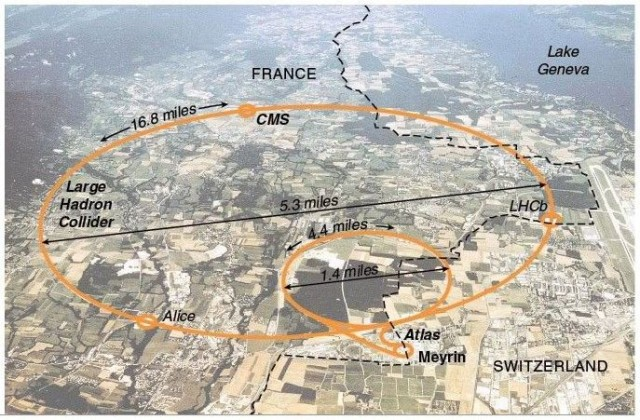
\includegraphics[width=.90\linewidth]{figures/lhc/lhc-5-640x420.jpg}
\caption{The \ac{LHC} main collider ring and pre-accelerator \ac{SPS} overlaid on a map of Switzerland and France, with the four main \ac{LHC} experiments identified.}
\label{fig:lhc_map}
\end{figure}
\end{centering}

%----------------------------------------------------------------------------------------

\section{The Injector Complex}

The goal of the \ac{LHC} is to provide high luminosity proton-proton collisions at 13 \tev. To achieve this, it must be capable of rapidly accelerating large numbers of protons and holding them at a constant energy, and organizing them into bunches which can be focused and collided at precise points and times. To do this, a complex system of pre-accelerators is required, as well as a precisely engineered sytem of magnets within the \ac{LHC}. The full system of pre-accelerators is shown in \autoref{fig:preacc}.

\begin{centering}
\begin{figure}[!hbt]
\myfloatalign
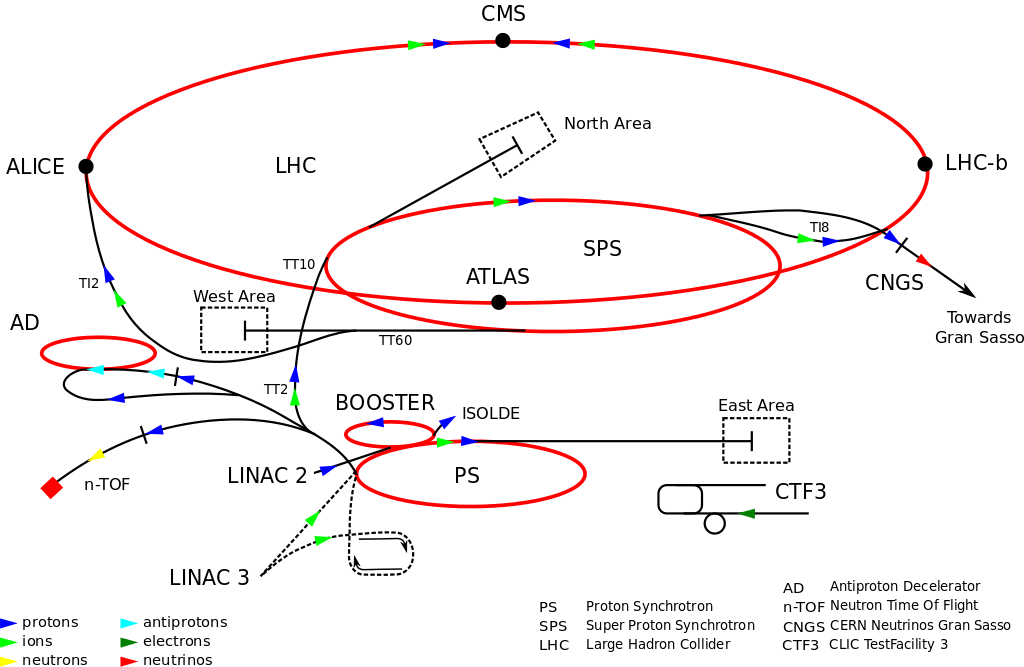
\includegraphics[width=.90\linewidth]{figures/lhc/Cern-accelerator-complex.png}
\caption{The pre-accelerators of the \ac{LHC}.}
\label{fig:preacc}
\end{figure}
\end{centering}

The chain begins with when hydrogen gas is stripped of its electrons and injected in short pulses into Linac2, a linear accelerator which uses \ac{RF} cavities, which use alternating positive and negative electric fields to simultaneously push and pull particles forward through the accelerator. This \ac{RF} behavoir keeps the bunches of protons resulting from the original pulses separated, beginning the formation of the bunch structure used for collisions. Quadropole magnets along the accelerator keep the beam focused. By the end of the accelerator, protons have reached 50 \mev. 

The proton beam is then injected into the \ac{PSB}, the first circular accelerator in the pre-accelerator chain. It increases its magnetic field as the protons increase in speed, ultimately accelerating them to 1.4 \gev. 

At this point the proton beam moves on to the \ac{PS}, a 600 m long circular accelerator that consists of 277 electromagnets that accelerate the protons up to 25 \gev, and 100 additional dipole magnets to bend the beam. 

The last accelerator before injection into the \ac{LHC} is the \ac{SPS}, a 7 km long ring which, long before the \ac{LHC} tunnel was built, was responsible for the discovery of the $W$ and $Z$ bosons. The \ac{SPS} accelerates particles up to 450 \gev~before they are launched into the \ac{LHC}. 

Proton bunches are structured for ease of acceleration, with distinct features resulting from each of the pre-accelerators. The \ac{PS} produces 72 bunches separated by 25 ns, which are injected into the \ac{SPS}, as seen in \autoref{fig:bunches}. However, as the magnetic field directing these protons out of the \ac{PS} loop is turned on, there must be a gap in the bunch structure. Without this gap, called the injection kicker rise time, the changing magnetic field would direct particles out of the accelerator and produce high amounts of unsafe radiation around the \ac{PS}. A similar gap in bunch structure is required for the injection from the \ac{SPS} to the \ac{LHC}. The injection process is repeated until the \ac{LHC} is completely filled with around 2000 bunches, which takes about three minutes.

\begin{centering}
\begin{figure}[!hbt]
\myfloatalign
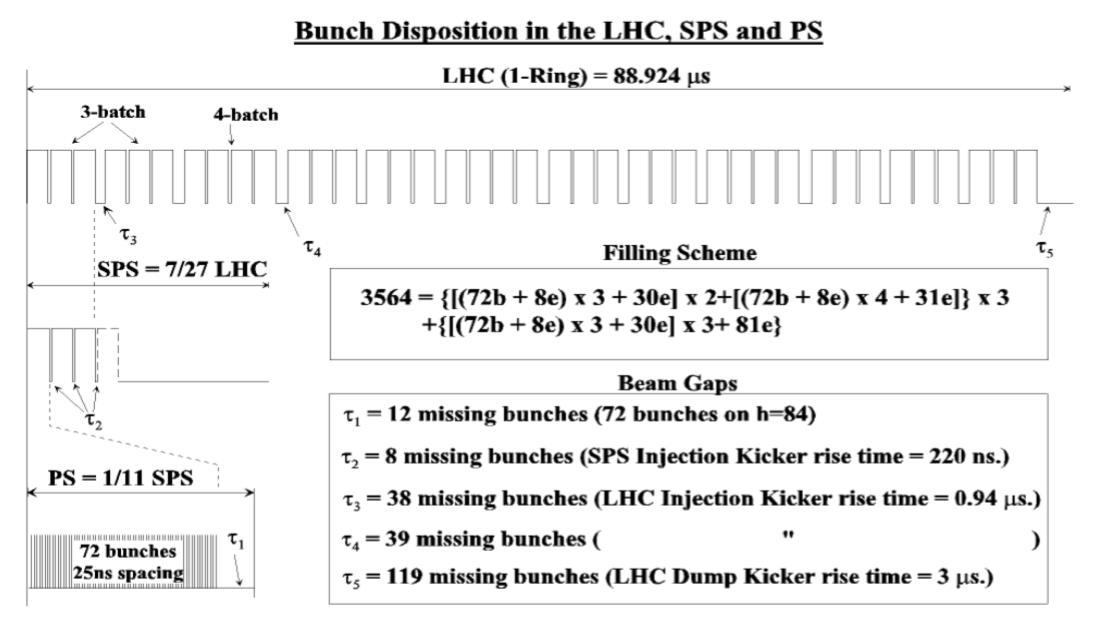
\includegraphics[width=.90\linewidth]{figures/lhc/bunch_structure.png}
\caption{Bunch structure in the \ac{PS}, \ac{SPS}, and \ac{LHC}.}
\label{fig:bunches}
\end{figure}
\end{centering}

\section{Operation of the Large Hadron Collider}

The \ac{LHC} consists of eight straight sections each connected by an arc. In each straigh section, \ac{RF} cavities accelerate protons, ultimately bringing them up to 6.5 \gev. Between these straight sections, 8.4 T dipole magnets bend the beams to maintain the approximately circular path. However, because the \ac{LHC} is a proton-proton collider as opposed to a proton-antiproton collider, the two counter-rotating beams must be housed in separate rings and be accelerated separately. To achieve this, twin-bore superconduncting magnets, one example of which can be seen in \autoref{fig:magnet}, surround the two rings and accelerate them both. Quadropole magnets are used at the four collision points to focus the beams, which cross at an interaction point at the center of a detector. In total there are 1232  main dipole magnets over 5000 additional magnets, which are all are superconducting and kept below their critical temperatures by liquid helium cooling. 

\begin{centering}
\begin{figure}[!hbt]
\myfloatalign
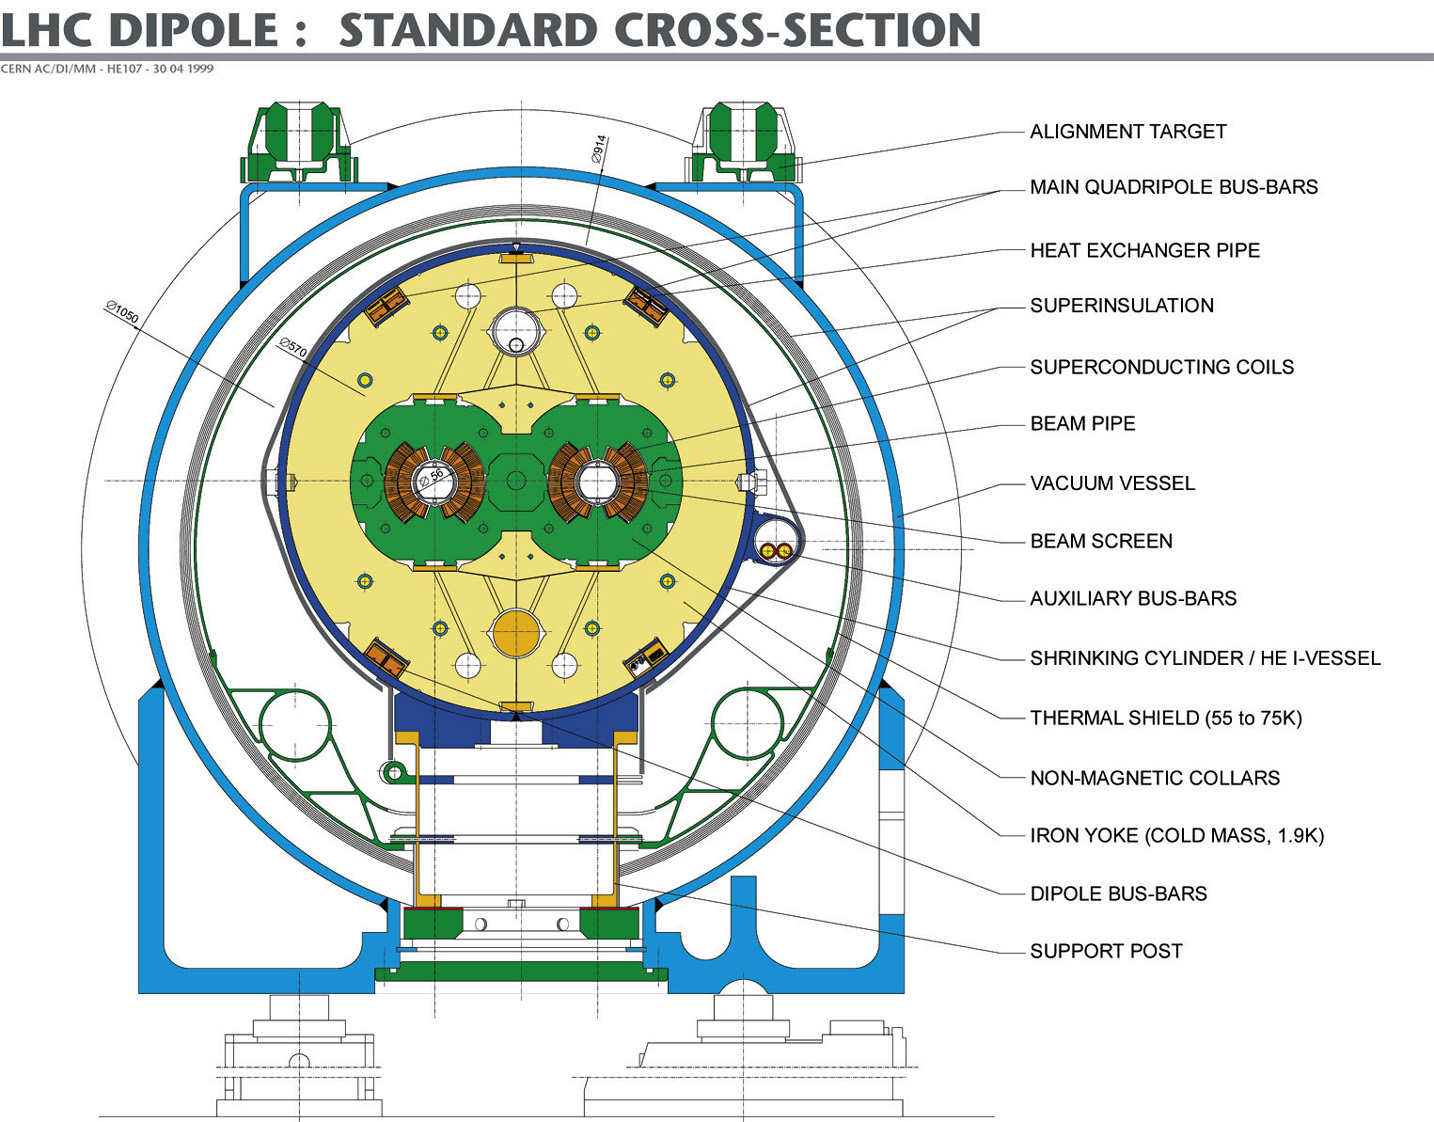
\includegraphics[width=.90\linewidth]{figures/lhc/magnet.jpg}
\caption{Cross-section of a cryodipole magnet in the \ac{LHC}.}
\label{fig:magnet}
\end{figure}
\end{centering}

When first injected into the \ac{LHC}, the protons must be accelerated over many turns through the machine, with the magentic field from the dipoles increasing with each pass to apply more force with which to bend the beam. Once the protons have reached a maximum energy, a process called ``squeezing'' occurs, in which the the total transverse area of the beam is reduced and bunches are elongated slightly. The shape produced by this process determines the ``beam spot'' for the ATLAS detector, the measurement of the area in which collisions occur within the detector. As shown in \autoref{fig:beam_spot}, the collisions all occur very close together in the $x-y$ plane, but have a long spread in the $z$ direction\footnote{The coordinate system used here is discussed in \autoref{sec:coords}.}.

\begin{centering}
\begin{figure}[!hbt]
\myfloatalign
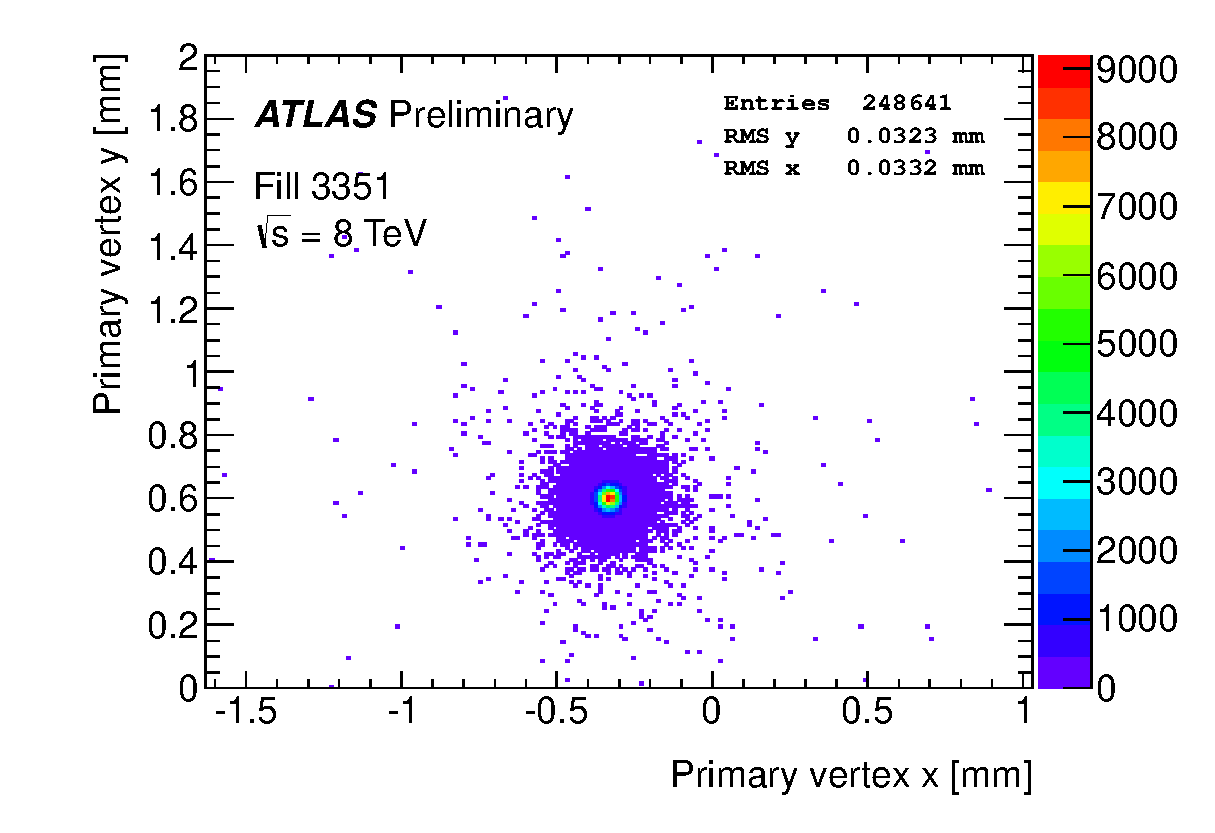
\includegraphics[width=.45\linewidth]{figures/lhc/beamspot-run215456-vtx-yx.eps}
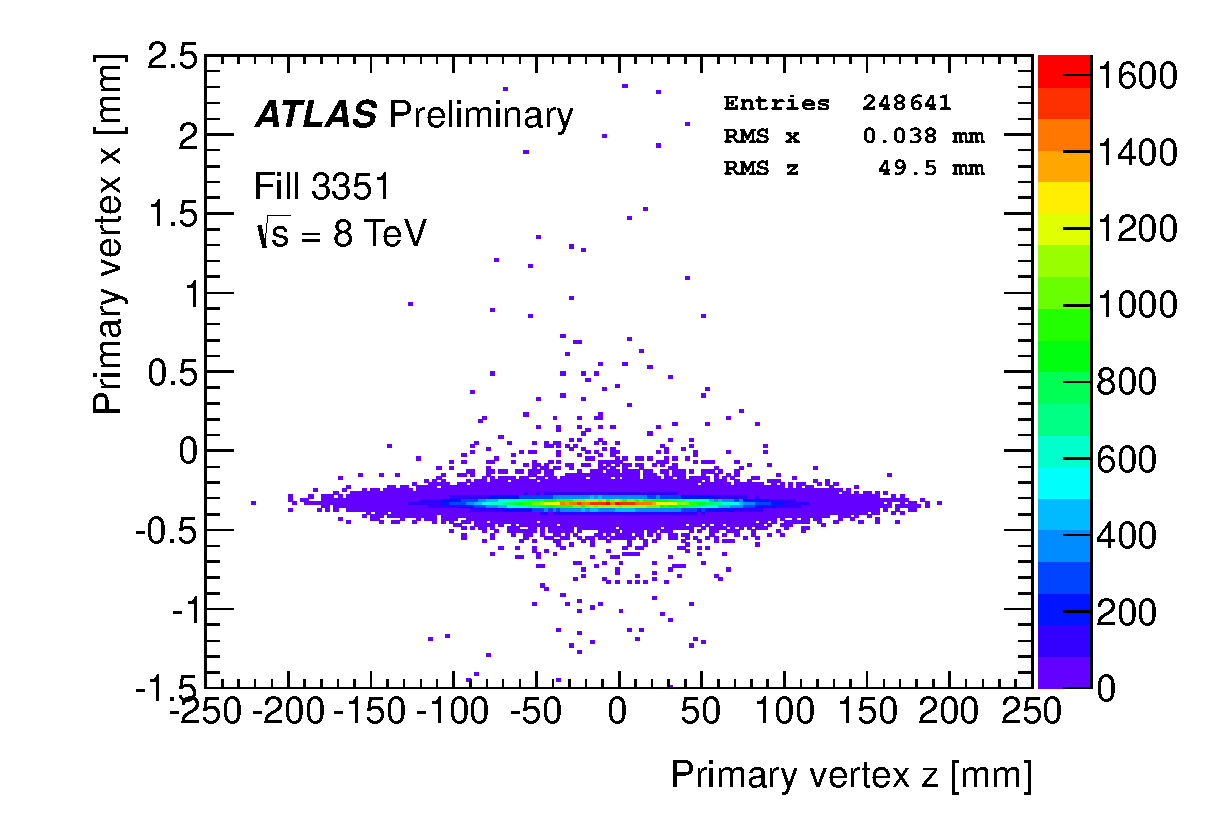
\includegraphics[width=.45\linewidth]{figures/lhc/beamspot-run215456-vtx-xz.eps}
\caption{Beam spot in the ATLAS detector for one run in 2015. Distributions show only the highest \pt vertex per event. Left is the $x-y$ distribution of vertices, while the right plot shows the $x-z$ distribution.}
\label{fig:beam_spot}
\end{figure}
\end{centering}

Once the beams are at a stable energy and have been squeezed, the \ac{LHC} indicates that it is physics-ready to the experiments around the ring, and, after some additional checks by each experiment, data-taking can begin. As collisons occur, the beam is depleted, and when it is sufficiently depleted to require a new fill, or if any instability occurs, the beam is dumped into a cavern filled with steel and concrete, which absorbs the energy. 

\section{Luminosity}

The goal of the collisions provided by the \ac{LHC} is to produce \ac{SM} and \ac{BSM} particles, which can be observed by the detectors. How frequently a given process could occur was a crucial consideration in its design. The number of events of a given type is given by

\begin{equation}
N_{event} = L\sigma_{event}
\end{equation}

where $L$ is the luminosity delivered by the \ac{LHC} and $\sigma_{event}$ is the cross-section of the process in question. These cross-sections vary over many orders of magnitude for different processes, as shown in \autoref{fig:cross_sections}, a plot of many different \ac{SM} cross-sections. As a consequence, a very large amount of luminosity is required to produce the more rare events, and to have enough statistical power to differentiate them from other much more common events.   

\begin{centering}
\begin{figure}[!hbt]
\myfloatalign
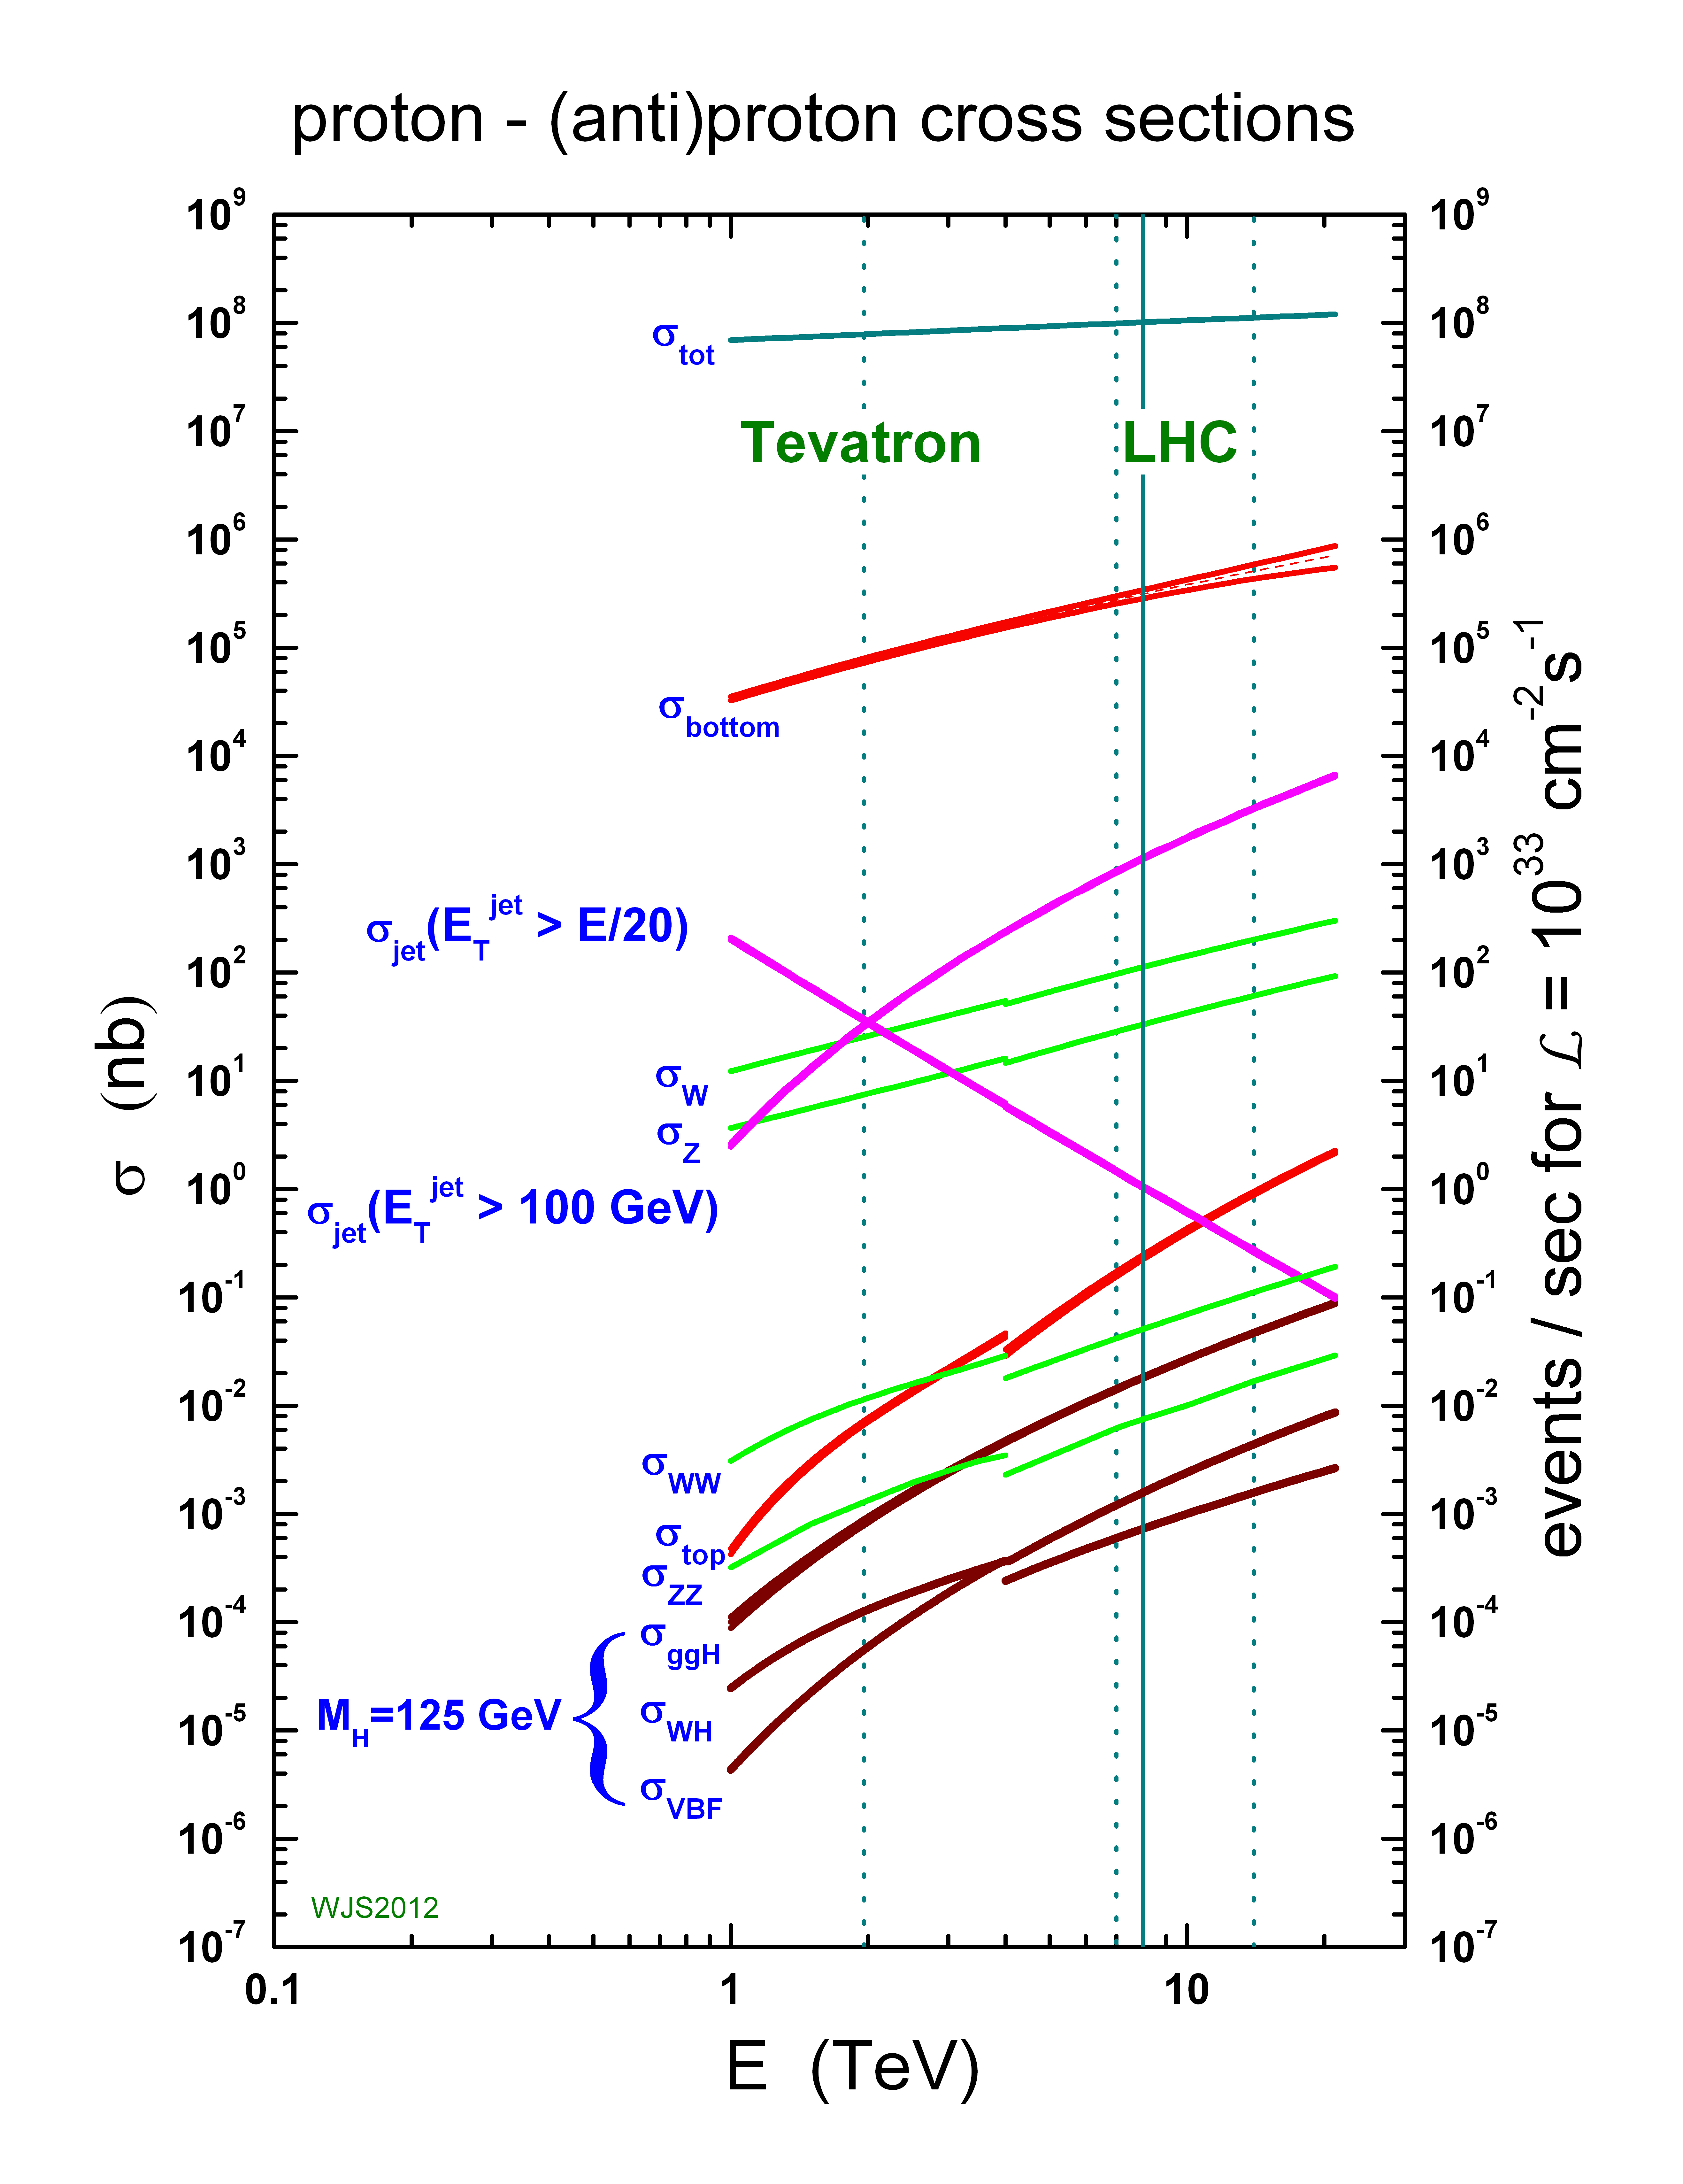
\includegraphics[width=.60\linewidth]{figures/lhc/crosssections2013.jpg}
\caption{Cross-sections for many \ac{SM} processes at the Tevatron and \ac{LHC} \cite{crosssections}.}
\label{fig:cross_sections}
\end{figure}
\end{centering}

The instantaneous luminosity at the \ac{LHC} is given by

\begin{equation}
L = \frac{ N^2_b n_b f_{rev} \gamma_r }{ 4\pi \epsilon_n \beta* } F
\end{equation}

where $N_b$ is the number of protons per bunch ($\sim10^{11}$), $n_b$ is the number of bunches in each beam ($\sim10^3$), $f_{rev}$ is the number of times per second that the beam travels around the ring, $\gamma_r$ is the relativistic gamma factor, $\epsilon_n$ is the normalized transverse beam emittance, and $\beta*$ is the $\beta$-function at the collision point, which describes the transverse displacement of particles in the beam. $F$ gives the reduction factor due to the geometry of the beam crossings, and is given by

\begin{equation}
F = (1+ (\frac{\theta_c \sigma_z}{2\sigma*})^2)^{-1/2}
\end{equation}

where $\theta_c$ is the crossing angle of the beams, $\sigma_z$ is the RMS of the bunch length in the $z$ direction, and $\sigma*$ is the same in the transverse direction.

As the proton beams circulate and collide, $N_b$ decreases, producing a falling instantaneous luminosity, as seen in a Run 1 example in \autoref{fig:instlumi}. In Run 2, peak instantaneous luminosity was brought up to $10^{34}$ cm$^{-2}$s$^{-1}$. This high instantaneous luminosity and consistent running resulted in much faster data collection than in Run 1, which is depicted in \autoref{fig:lumi_vs_year}. 

\begin{centering}
\begin{figure}[!hbt]
\myfloatalign
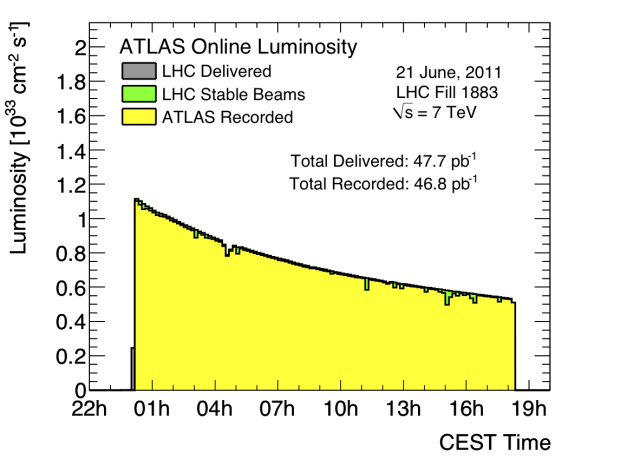
\includegraphics[width=.90\linewidth]{figures/lhc/lumi1883.jpg}
\caption{Instantaneous luminosity of one fill of 7 \tev data in 2011.}
\label{fig:instlumi}
\end{figure}
\end{centering}

\begin{centering}
\begin{figure}[!hbt]
\myfloatalign
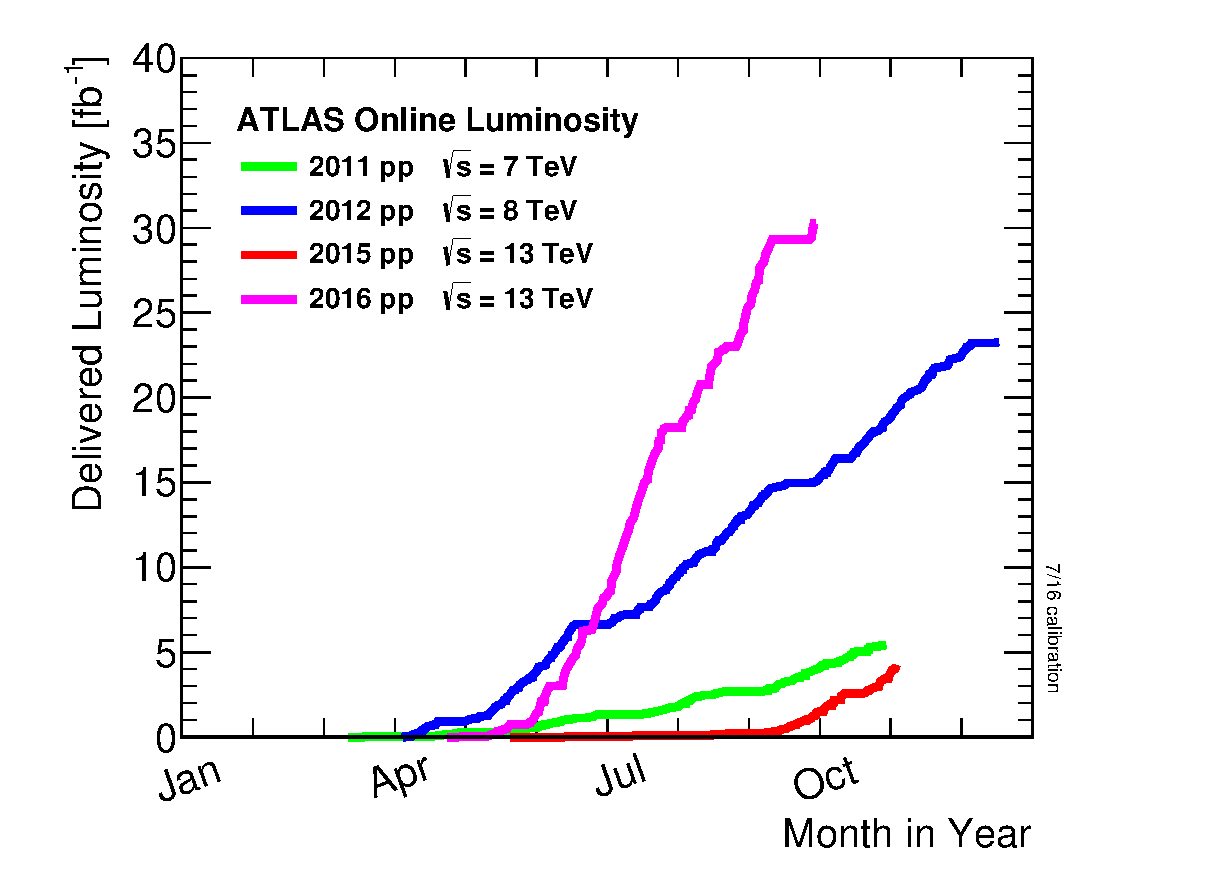
\includegraphics[width=.90\linewidth]{figures/lhc/intlumivsyear.eps}
\caption{ATLAS luminosity for Run 1 and Run 2, as of September 2016.}
\label{fig:lumi_vs_year}
\end{figure} 
\end{centering}

\section{Pile-up in proton-proton Collisions}
\label{sec:pileup}

One consequence of the high instantaneous luminosity is ``pile-up'', or multiple simultaneously interactions. Because each bunch has on order 100 billion protons, it is very likely that multiple protons will collide in the same bunch crossing. In fact, the average number of simultaneous interactions in 13 \tev data, shown in \autoref{fig:ninteractions}, is about twenty. 

\begin{centering}
\begin{figure}[!hbt]
\myfloatalign
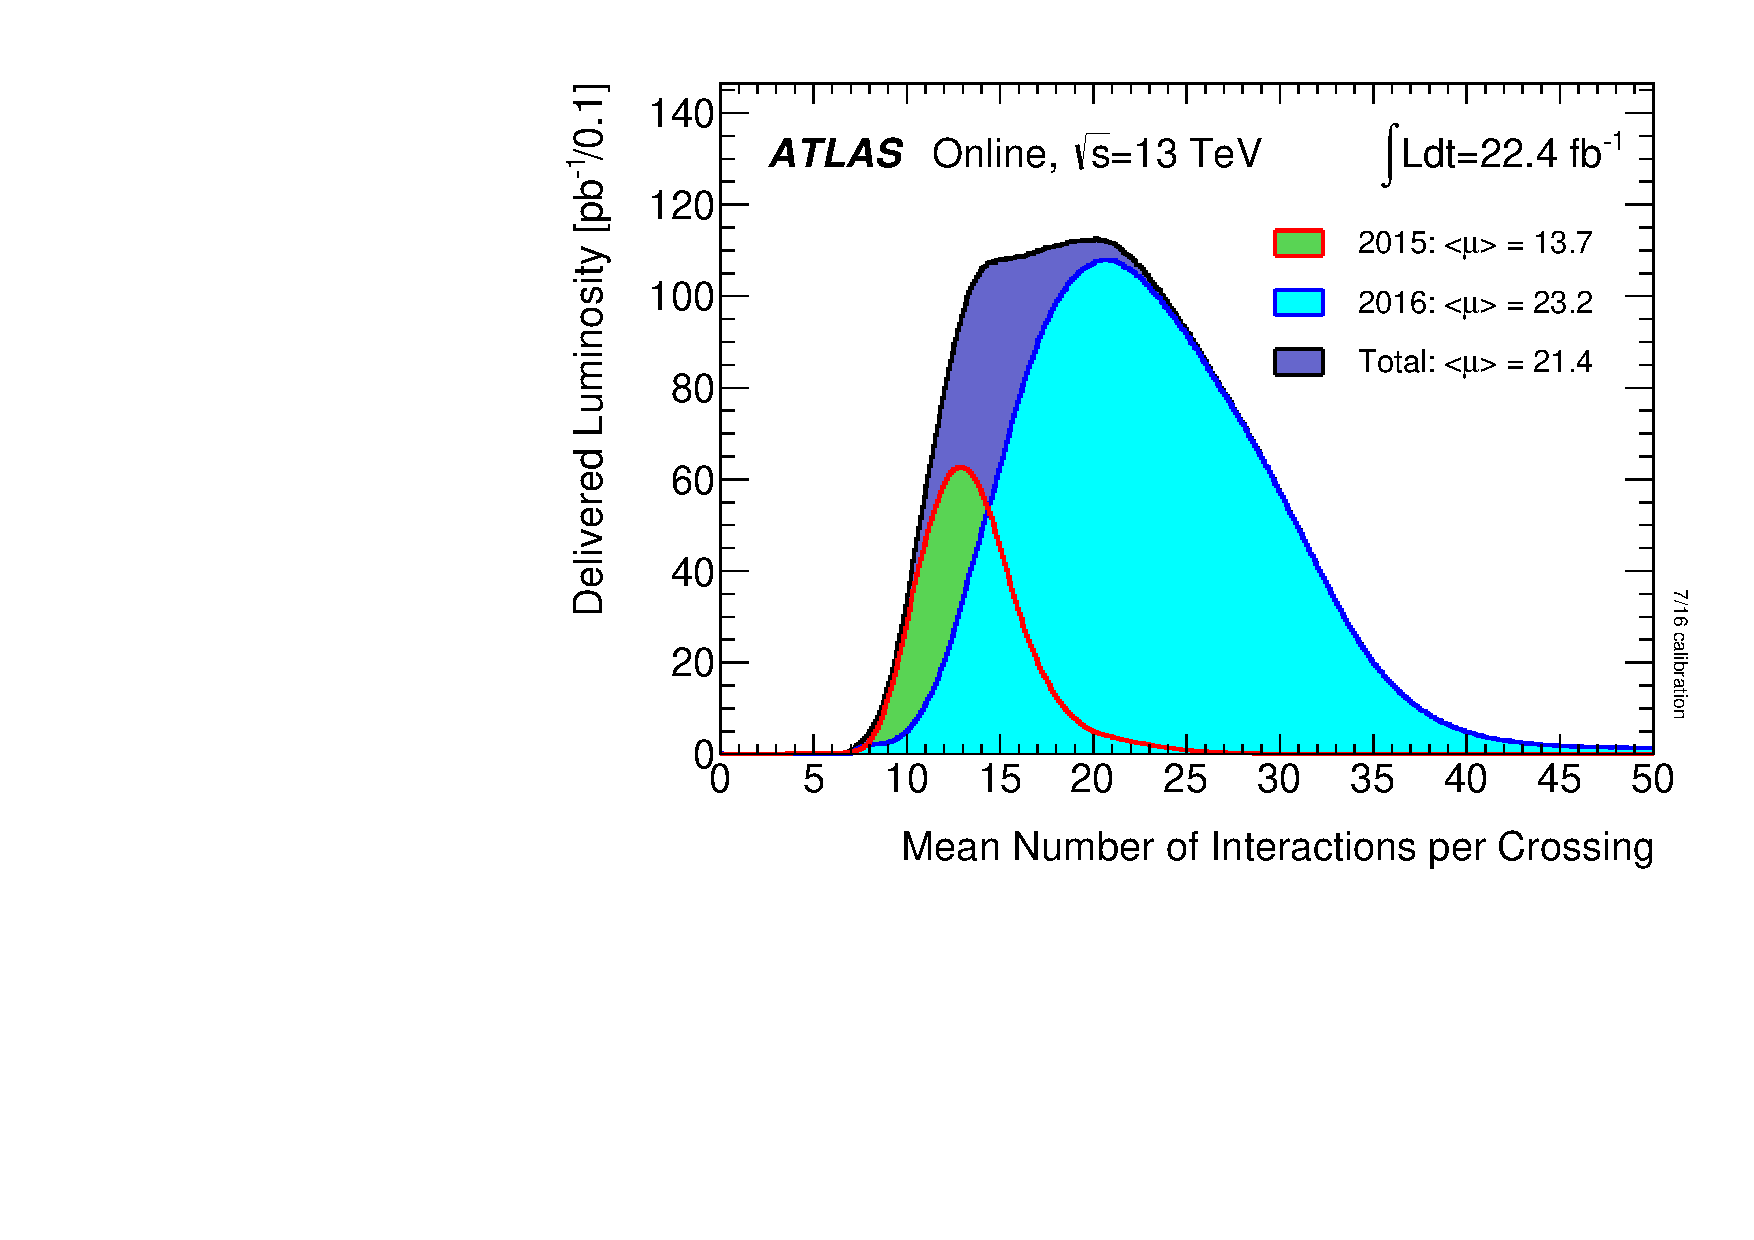
\includegraphics[width=.85\linewidth]{figures/atlas/mu_2015_2016_ICHEP.pdf}
\caption{Average number of interactions per crossing shown for 2015 and 2016 separately, as well as the sum of the two years.}
\label{fig:ninteractions}
\end{figure}
\end{centering}

Pile-up can be a difficult challenge for the ATLAS collaboration because it typically results in additional jets in an event, and can increase \ac{SM} backgrounds for analyses seeking to identify events with jets. It can also add to the overall hadronic energy of an event, and that energy can be mis-assigned to other objects. Fortunately, it is typically possible to resolve the different vertices that each proton-proton collision makes, and so pile-up jets can be identified and rejected. 


 % LHC
% Chapter X

\chapter{The ATLAS Detector} % Chapter title

\label{ch:atlas} % For referencing the chapter elsewhere, use \autoref{ch:name} 

The ATLAS detector circumscribes the \ac{LHC}'s beam pipe, enclosing the collision point with a series of particle detecting layers, aimed at making as many measurements of the particles leaving the collision point as possible. Its goal is to get a precise measurement of all the stable or semi-stable particles flying from proton-proton collisions at its center, allowing analyzers to fully reconstruct the kinematics of the underlying processes.

The ATLAS detector is the largest detector of its kind, measuring 44 m in length and 25 m in height, as seen in \autoref{fig:detector}. The size is mainly determined by the constraints of the \ac{MS}, discussed in \autoref{sec:MS}, which is the largest and outermost subsystem. The \ac{MS} is submerged in a spatially varying magnetic field provided by three toroidal magnets, while the \ac{ID} (\autoref{sec:ID}) is encased by a superconducting solenoid, which provides a uniform 2 T field throughout its volume \cite{PERF-2007-01}.

\begin{centering}
\begin{figure}[bth]
\myfloatalign
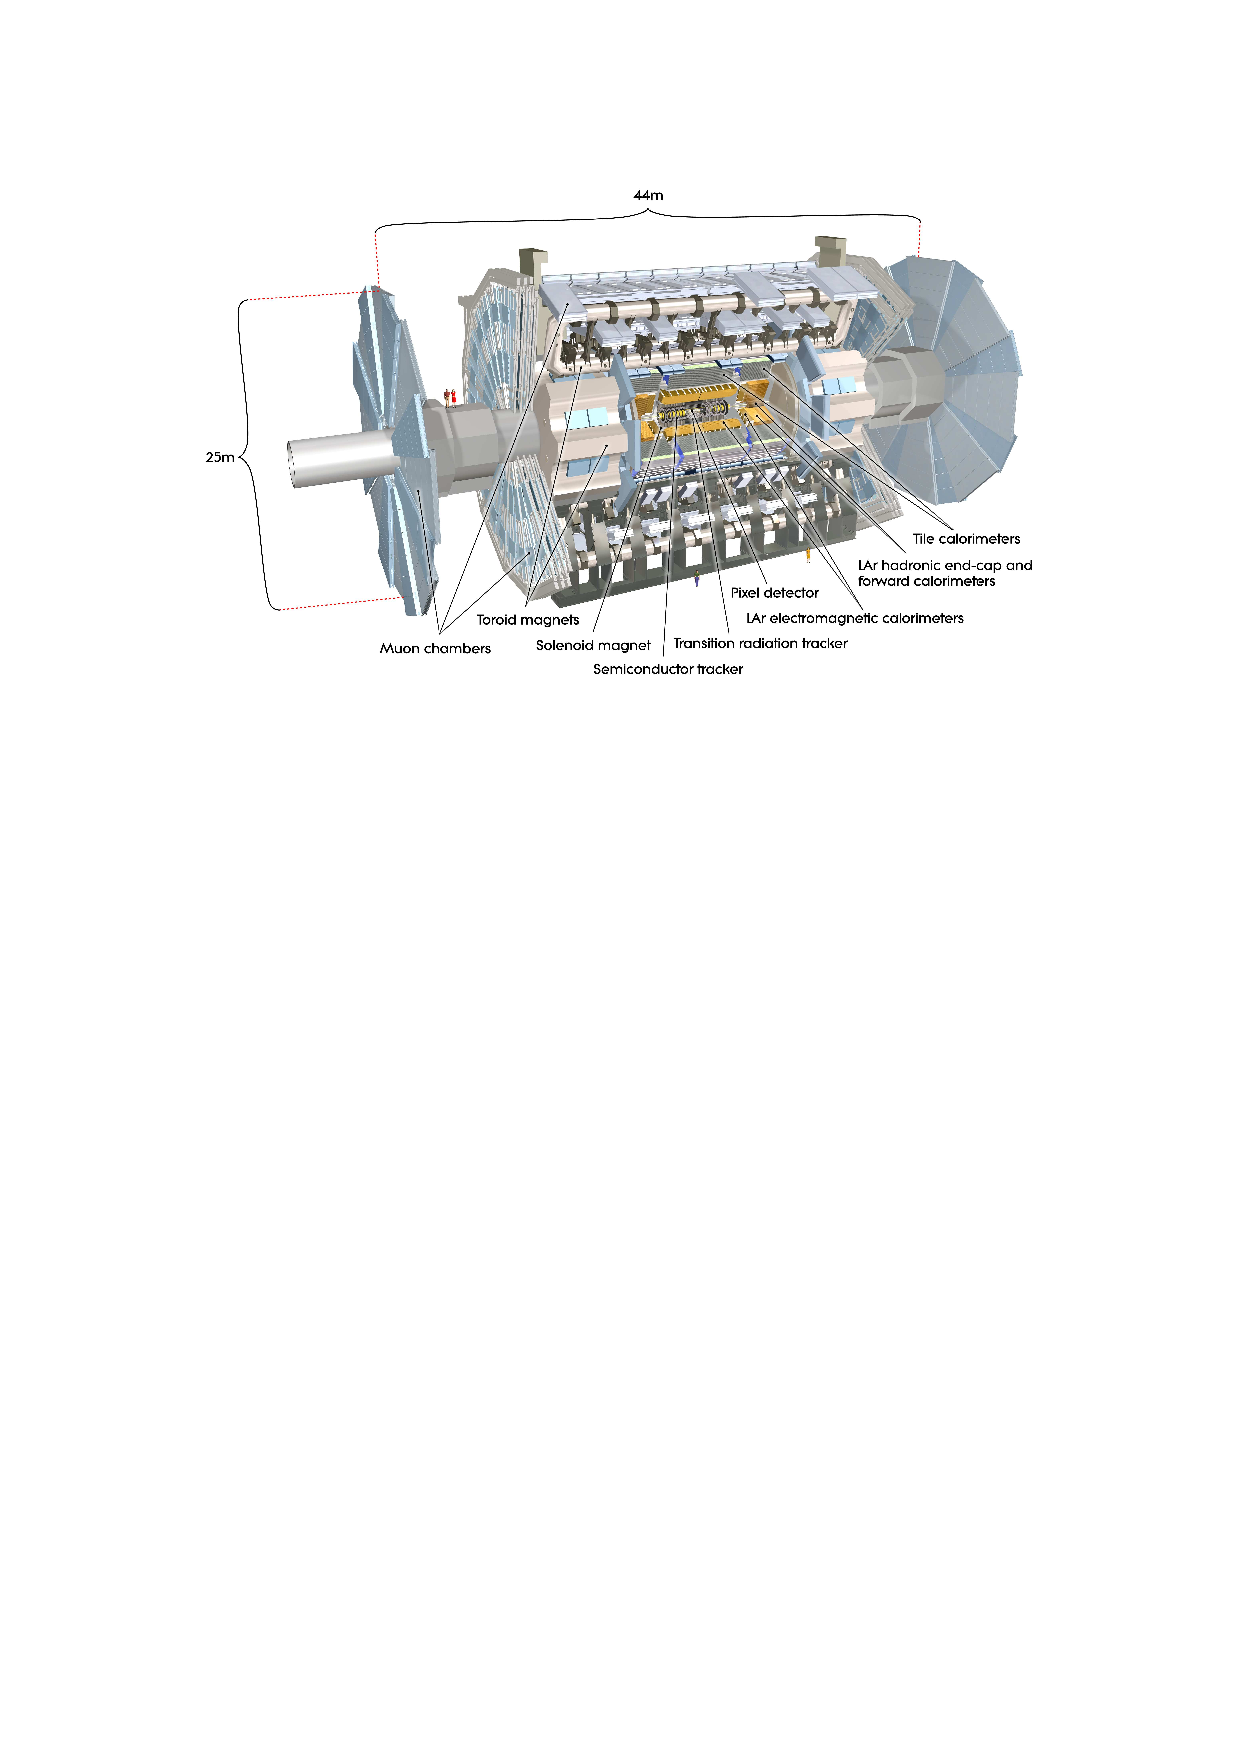
\includegraphics[width=.90\linewidth]{figures/atlas/detector.pdf}
\caption{Diagram of the ATLAS detector, with subsystems and magnets identified.}
\label{fig:detector}
\end{figure}
\end{centering}

\section{Coordinate System Used in the ATLAS Detector}

The ATLAS detector is centered around a the collision point in the beam pipe, and is built radially out from the pipe, maintaining as much rotational symmetry as possible. It is also symmetric in the forward-backward directions. Because of this geometry, a coordinate system using the collision point as the origin is used, with the beam pipe defining the $z$-axis. The positive $x$ direction is defined as pointing to the center of the \ac{LHC} ring, while the positive $y$ direction points upwards. For ease of reference, the side of the detector in the positive-$z$ direction is referred to as the A side, and the other side is referred to as the C side. 

Because of the radial design of the detector, angular coordinates are often used. The azimuthal angle $\phi$ defines the radial distance around the beam pipe and the polar angle $\theta$ defines the angle from the beam axis ($z$). However, a transformation of the polar angle called pseudorapidity ($\eta$) is used more often, and is defined as 

\begin{equation}
\eta = - ln [ tan \frac{\theta}{2} ]. 
\end{equation}

Building on this variable definition, distance between objects is typically defined as

\begin{equation}
\Delta R = \sqrt{\Delta\eta^2 + \Delta\phi^2}. 
\end{equation}

Often variables are defined purely in the transverse plane, which is indicated by a subscripted $T$, as in $p_T$, which gives an object's transverse momentum. Another common usage is $E_T^{miss}$, which gives the negative vectorial sum of the energy in an event. 

%------------------------------------------------

\section{The Inner Detector}
\label{sec:ID}

One goal of the ATLAS detector is to produce tracks, predictions of the paths particles take as they travel through the detector. Collisions in the detector produce about 1000 particles, so identifying and differentiating all these tracks is both a hardware and a computational challenge. The \ac{ID}, also called the Tracker, is responsible for providing high enough resolution measurements that each of these tracks and its precise position can be recorded. This tracking system consists of three subdetectors which each produce electrical responses to charged particles passing through their active material. Each of these signals is called a hit. ATLAS tracking software considers all these hits and forms tracks, with the goal of minimizing fake tracks due to random noise. Some details of this process is discussed at length in \autoref{sec:NN}. The full \ac{ID} can be seen in \autoref{fig:ID}, while a schematic in \autoref{fig:IDeta} demonstrates the $\eta$ coverage of each detector.

\begin{centering}
\begin{figure}[bth]
\myfloatalign
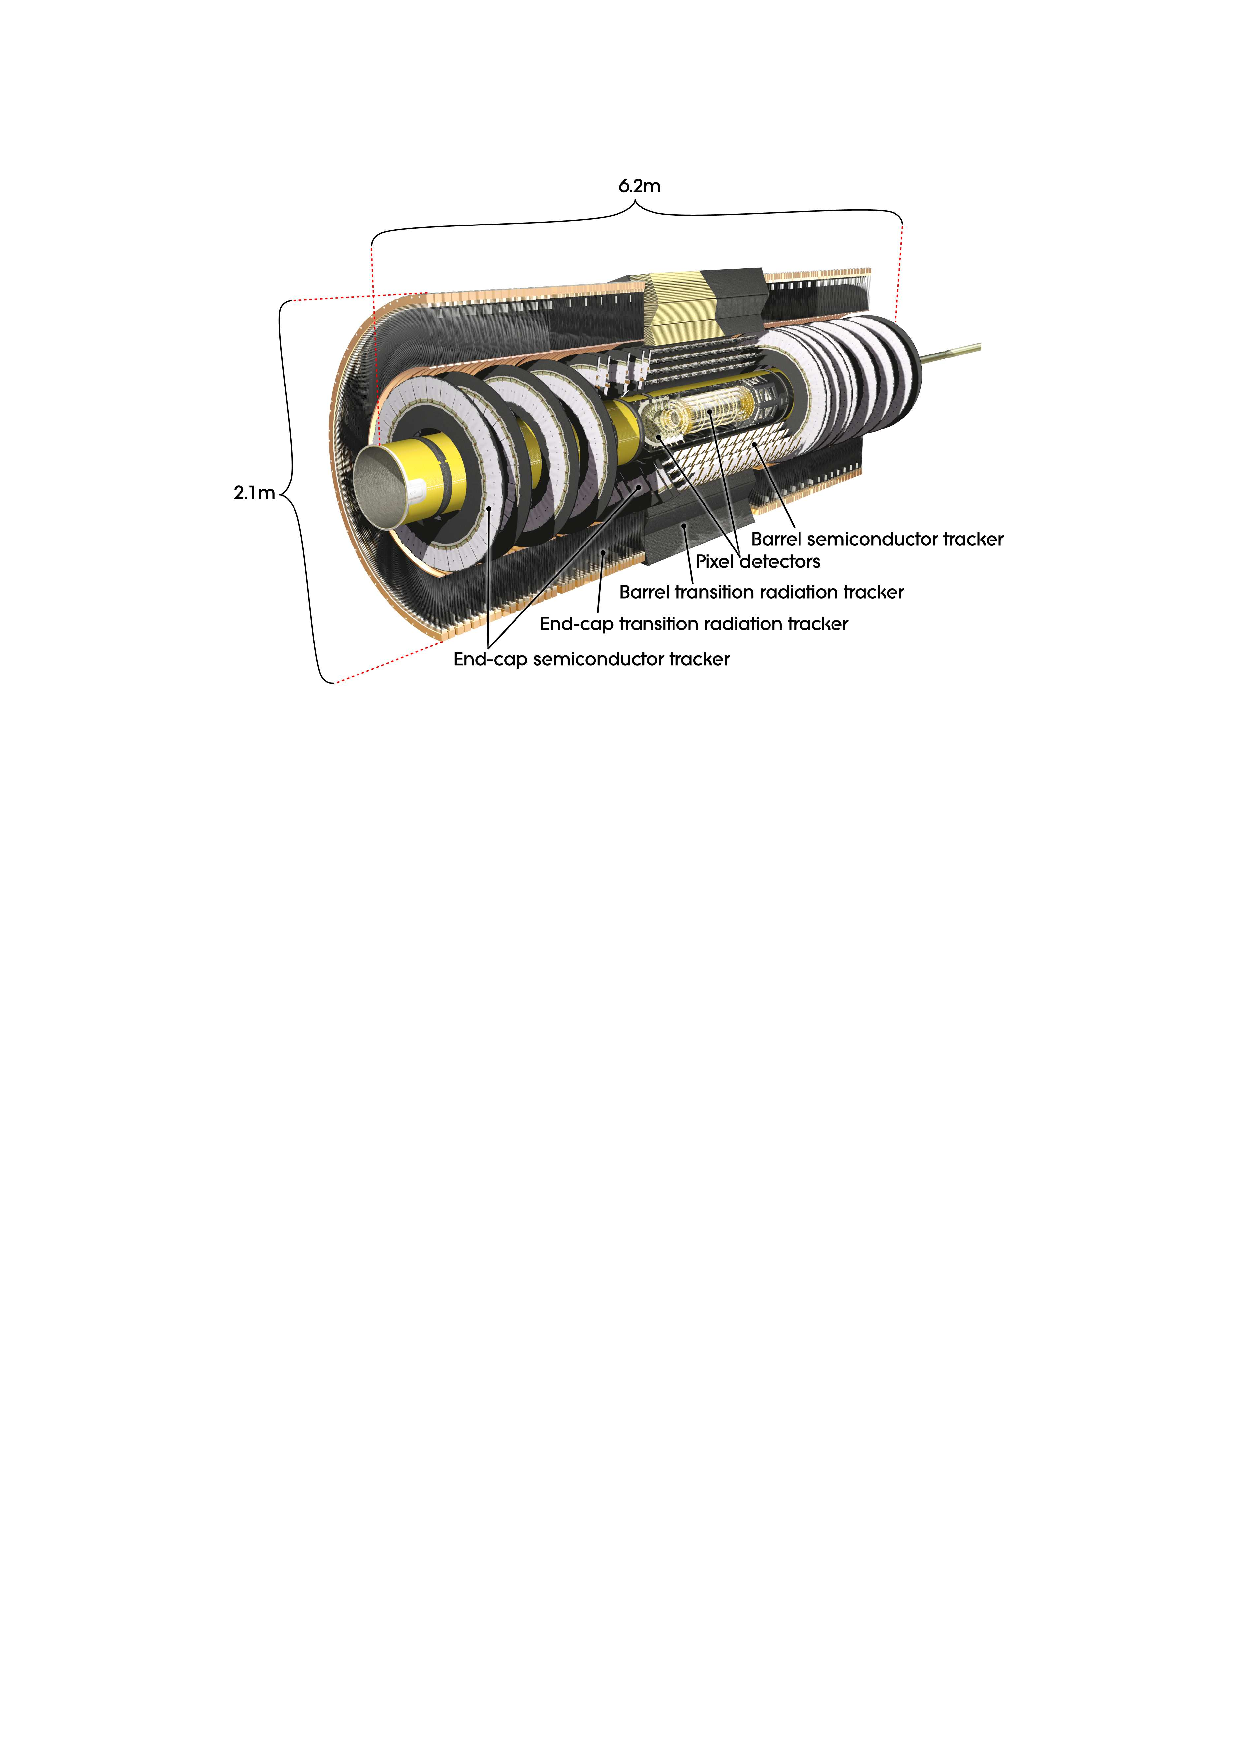
\includegraphics[width=.90\linewidth]{figures/atlas/innerdetector.pdf}
\caption{Diagram of the ATLAS Inner Detector, containing the Pixel, SCT, and TRT subsystems.}
\label{fig:ID}
\end{figure}
\end{centering}

\begin{centering}
\begin{figure}[bth]
\myfloatalign
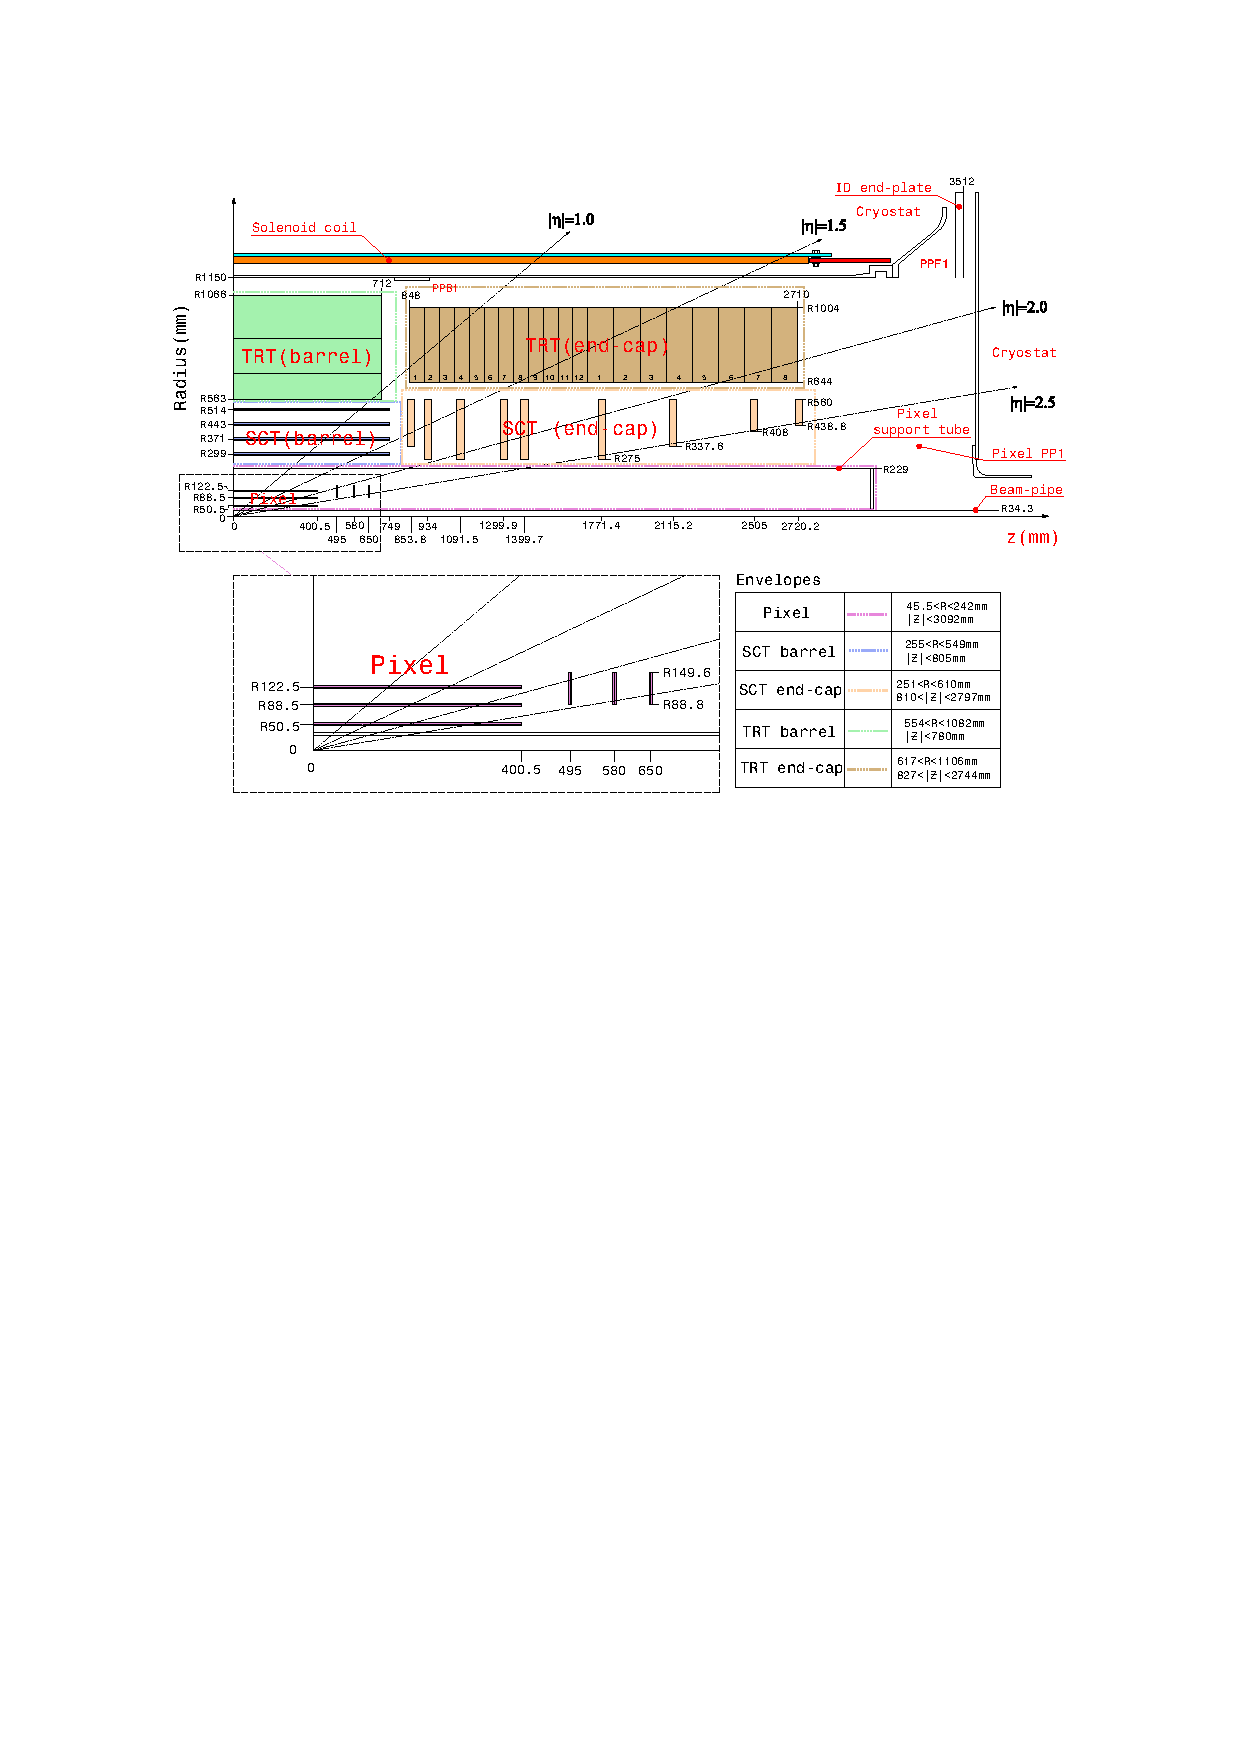
\includegraphics[width=.90\linewidth]{figures/atlas/ideta.pdf}
\caption{Diagram of one-quarter of the ATLAS Inner Detector, with lines drawn to indicate various $\eta$ locations. The labels PP1, PPB1 and PPF1 indicate the patch-panels for the ID services. TODO: what is that.}
\label{fig:IDeta}
\end{figure}
\end{centering}

\subsection{The Pixel Detector}

The Pixel detector lies closest to the beam pipe of the \ac{LHC}, and has four layers comprising 92 million read-out channels. There are three standard layers, referred to as Layers 1-3 (L1, L2, L3), and an additional layer added for the 2015 data-taking, called the \ac{IBL}. 

\subsubsection{The Original Pixel Detector}

The Pixel Detector consists of high-precision silicon chip pixel sensors, with 1744 sensors total. Each sensor is identical, containing 47232 pixels, which are typically each 50$\times$400 $\mu$m$^2$. 

As shown in \autoref{fig:IDeta}, the central $\eta$ region (barrel) is covered by three concentric cylindrical layers of sensors, while the higher $\eta$ region (endcap) is covered by a series of three disks positioned in the $x-y$ plane. Together, they give complete coverage out to $\eta = 2.5$, and a particle coming from the collision point will typically by measured by three layers. Each of these measurements is accurate in the barrel (endcap) to 10 $\mu$m in the $R-\phi$ direction and 115 $\mu$m in the $z$ ($R$) direction.  

\subsubsection{Addition of the IBL}

In 2015, the \ac{IBL} was lowered into the ATLAS cavern and added to the Pixel Detector. This layer sits on top of the beam pipe, inside barrel L1, which was formerly responsible for the first measurement of charged particles coming from a collision. 
TODO: add info about precision 


As the \ac{IBL}'s' name suggests, it was added to improve detection of $B$ mesons, whose non-trivial lifetimes create secondary vertices in ATLAS events, which allow them to be distinguished from other particles with precise track measurement. The \ac{IBL} is closer to the interaction point and has a smaller resolution, giving it a better chance to see these slightly displaced vertices.

\subsection{The Silicon Microstrip Tracker}

The \ac{SCT} employs similar technology to the Pixel Detector, with 15912 sensors and 6.3 million readout channels. Its difference from the Pixel Detector is in the readout, which is performed by a series of 12 cm long strips with a width of 80 $\mu$m. These layers are paired, placed on top of one another at a small (40 mrad) angle to allow for position determination in both directions, giving 4 spatial measurements for each particle passing through the \ac{SCT}. In the barrel, these strips run parallel to the beam pipe, while in the endcap, they are arranged radially. These strips have a resolution in the barrel (endcap) of 17 $\mu$m in the $R-\phi$ direction and 580 $\mu$m in the $z$ ($R$) direction. 

\subsection{The Transition Radiation Tracker}

The \ac{TRT} uses 4mm diameter gas-filled tubes, each with a high voltage wire suspended along the center of the tube. The tubes run the length of the barrel, with a separate wire in the positive and negative $z$ direction. In the endcap, the tubes are arranged radially. In total, there are about 351,000 readout channels in the \ac{TRT}. This detector makes measurements only in the $R-\phi$ direction, where the resolution of each measurement is 130 $\mu$m. Each particle typically creates about 36 hits as it passes through the \ac{TRT}. 

Particles passing through the gas mixture of the \ac{TRT} ionize the gas, producing electrons which drift towards the wire due to a potential difference applied between it and the straw. The \ac{TRT} also responds to low-energy transition radiation photons, which produce a much larger signal than charged particles passing through the detector. Because of this strong difference in signals, hits from the \ac{TRT} are used to help differentiate between electrons and photons in the detector.

\section{The Calorimeters}
\label{sec:Calo}

Unlike the tracking detectors, which aim to take measurements of a particle with minimal alterations of its trajectory, the calorimeters measure the the energy of objects by stopping them entirely. The calorimeters, which can be seen in \autoref{fig:calo}, provide coverage out to $\eta$ < 4.9. Higher granularity electromagnetic measurements are made within $|\eta|$ < 2.5, where the \ac{ID} provides tracking capability, in order to give precision measurements of the energy of photons and electrons, and provide reduced resolution measurements at higher $\eta$. The hadronic calorimeters provides coarser granularity, which is sufficient to determine the energy of jets. 

\begin{centering}
\begin{figure}[bth]
\myfloatalign
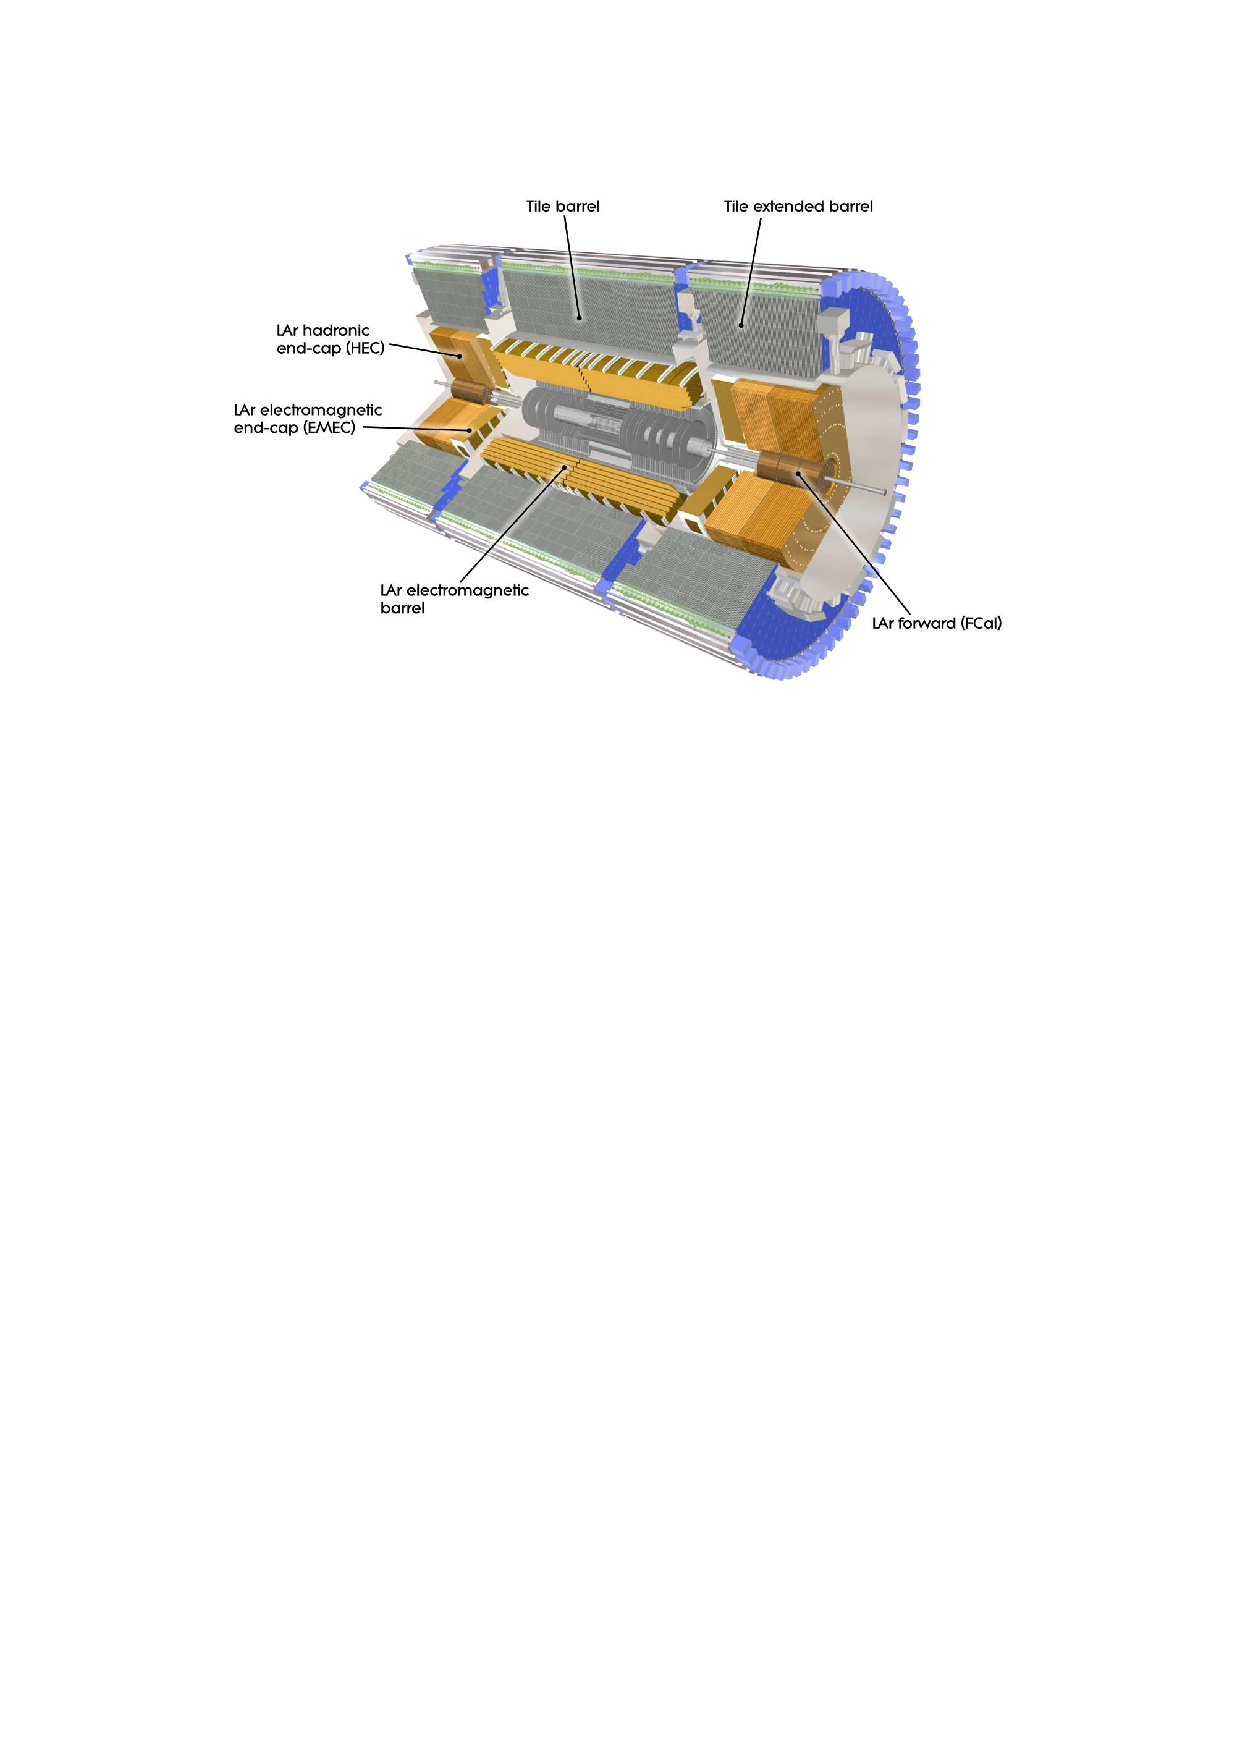
\includegraphics[width=.90\linewidth]{figures/atlas/calorimeters.pdf}
\caption{The calorimeter system of the ATLAS detector.}
\label{fig:calo}
\end{figure}
\end{centering}

%TODO make sure jets are in theory.

Another task of the calorimeter system is to limit punch-through to the \ac{MS}, described in \autoref{sec:MS}. All other particles must be fully stopped by the calorimeters to allow for clean signals from muons, and to measure the total energy of the particle. This requirement sets minimum sizes for each of the calorimeters. 

\paragraph{The LAr Electromagnetic Calorimeter} uses liquid argon as its active detector medium alternating with layers of lead acting as the absorber. The layers are shaped like accordions, which allows for complete coverage with multiple layers of active material, three in central $\eta$ ($0<|\eta|<2.5$) and two at higher $\eta$ ($2.5 < |\eta| < 3.2$). At $|\eta| < 1.8$, an instrumented liquid argon presampler provides a measurement of energy lost prior to reaching the calorimeters.

\paragraph{The Tile Calorimeter} is a hadronic calorimeter which surrounds the LAr Calorimeter. It uses layers of steel as its absorber with scintillating tiles as the active material between them, which are read out by photomultiplier tubes. The Tile Calorimeter covers $|\eta| < 1.7$. 

\paragraph{The LAr Hadronic Endcap Calorimeter} covers the hadronic calorimetery for higher $\eta$. It uses liquid argon active material and copper plate absorbers. This calorimeter covers $1.5 < |\eta| < 3.2$, overlapping with the hadronic calorimeters in either direction of its $\eta$ range. 

\paragraph{The FCal} or forward calorimeter provides electromagnetic and hadronic coverage at very high $\eta$ ($3.1 < |\eta| < 4.9$). This calorimeter also uses liquid argon as its active material, and uses copper-tungsten as the absorber. 

\section{The Muon Spectrometer}
\label{sec:MS}

The \ac{MS} measures charged particles that escape from the calorimeter system. Because the calorimeters are designed to completely absorb the energy of electrons, photons, hadrons, and jets, the \ac{MS} mainly detects muons, which escape from the calorimeter with very little loss of energy. The goal of the \ac{MS} is to give a high-precision measurement of these muons, and also to be able to quickly identify events with muons for the sake of triggering, discussed in \autoref{sec:Trigger}. The layout of the \ac{MS} can be seen in \autoref{fig:muon_xy} and \autoref{fig:muon_rz}. Muons can be measured for all $|\eta|$<2.7, and they can be triggered on for $|\eta|$<2.4. The entire system is about 24m tall and 40m long. 

\begin{centering}
\begin{figure}[bth]
\myfloatalign
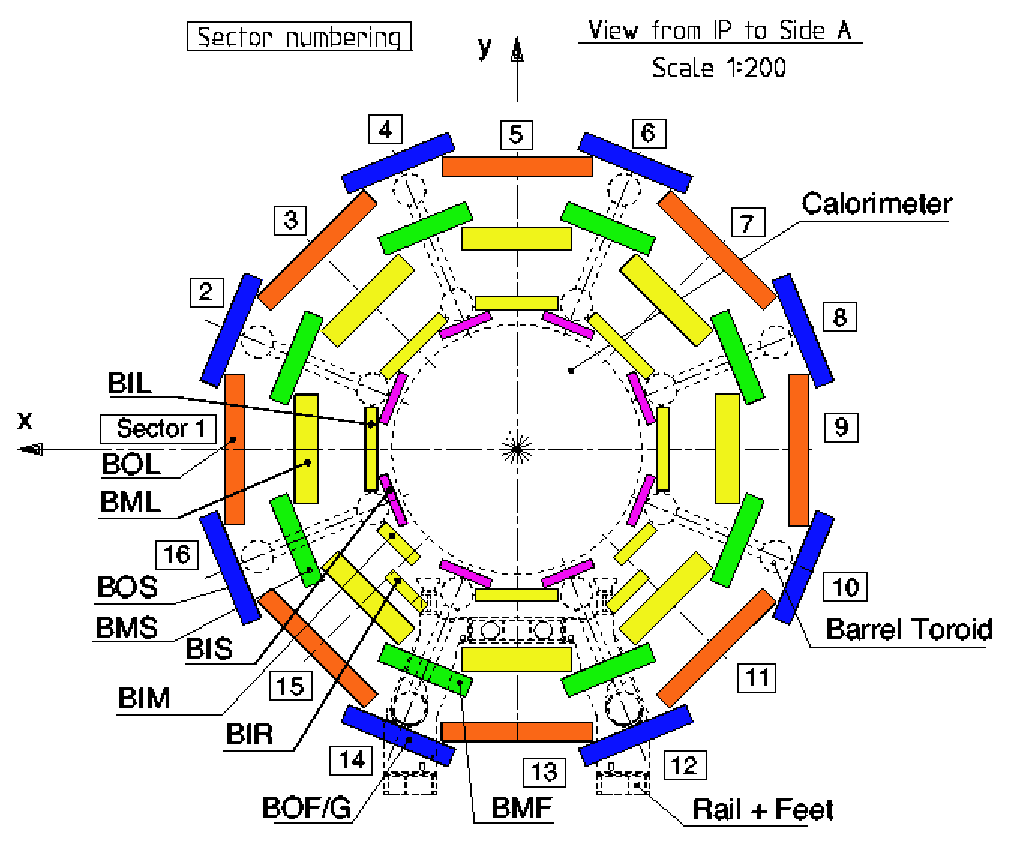
\includegraphics[width=.90\linewidth]{figures/atlas/Muon_sector_numbering.eps}
\caption{An $x$-$y$ view of the \ac{MS}. In it, the three barrel layers are visible, as well as the overlapping, differently sized chambers. The outer layer of the \ac{MS} is about 20m in diameter.}
\label{fig:muon_xy}
\end{figure}
\end{centering}

\begin{centering}
\begin{figure}[bth]
\myfloatalign
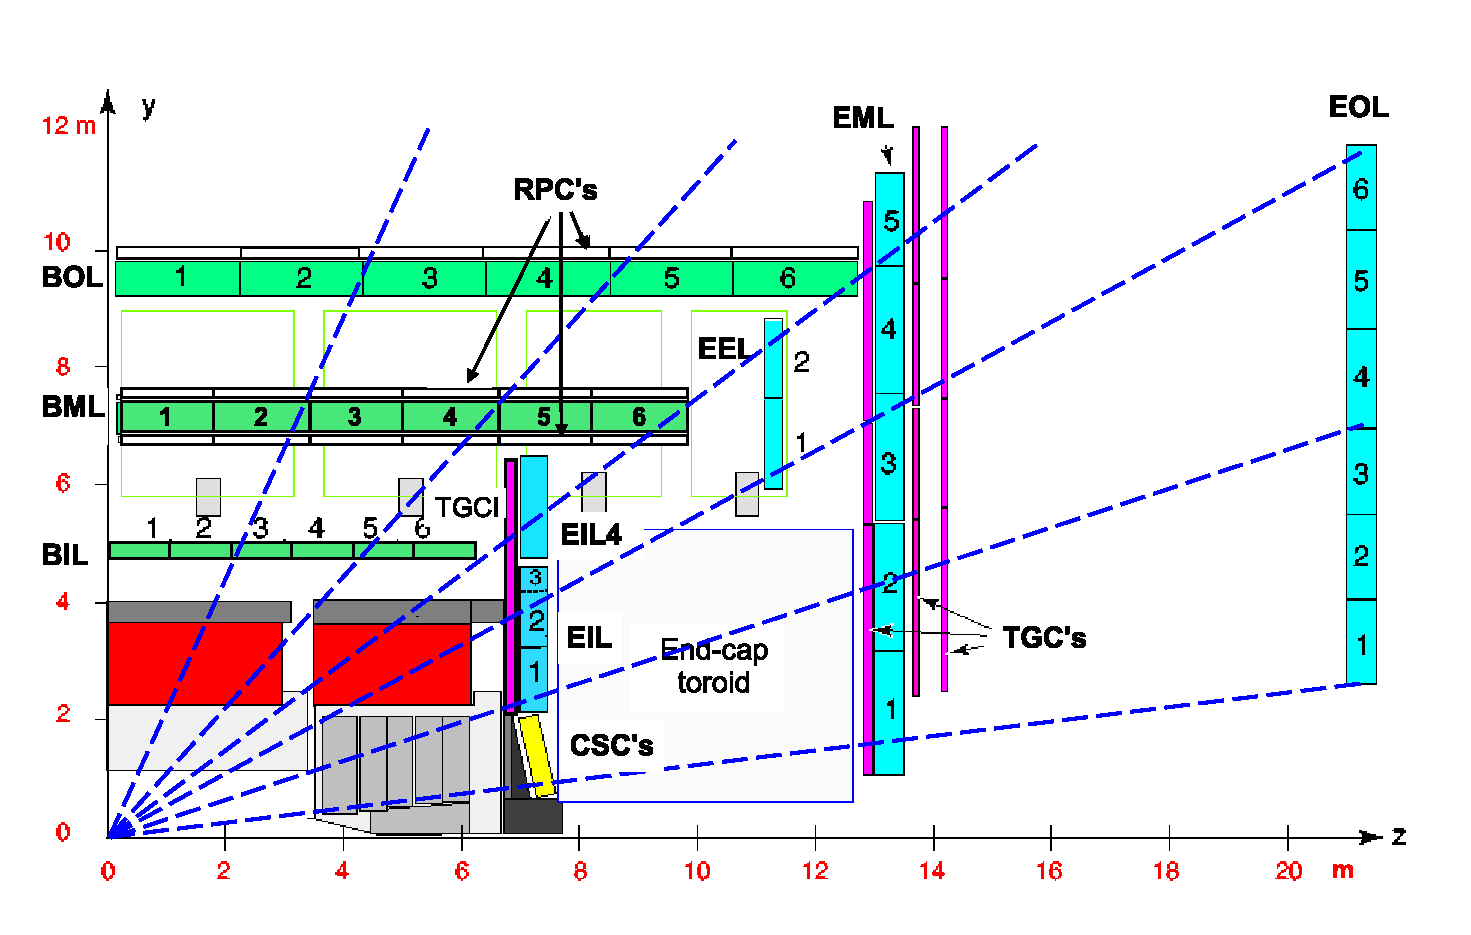
\includegraphics[width=.90\linewidth]{figures/atlas/Muon_rz_large_sect_6.eps}
\caption{An $r$-$z$ view of the \ac{MS}. The three layers of the barrel and endcap \ac{MS} are visible, and all muons at $|\eta|$<2.7 should traverse three detectors, assuming they propagate in an approximately straight line from the interaction point.}
\label{fig:muon_rz}
\end{figure}
\end{centering}

To achieve these goals, the \ac{MS} has several subsystems. The system responsible for precision measurement is called the \acp{MDT}. This subdetector consists of chambers of three to eight layers of tubes, with three layers of chambers covering both the barrel and end-cap regions. The tubes each contain an Ar/CO$_2$ gas mixture and a single high voltage wire which runs at its center along its length. Charged particles excite the gas as they pass through it, producing electrons which drift towards the high voltage wire. The resulting electric signal is read out, and the magnitude and timing of the signals are both used to differentiate particle traces from noise. 

Though very effective at giving a precise measurement, the \acp{MDT} have several shortcomings. The first is that the measurement is only precise in the direction perpendicular to the tubes; in the direction parallel to them, the resolution is not much better than the length of the drift tube. The resolution in the perpendicular direction is about 35 $\mu$m with the combined measurement of all the tubes in a chamber. 

The \acp{MDT} are slow, with a maximum drift time of about 700ns. Because collisions occur every 25ns, this readout cannot be used for triggering. In addition, in high-rate regions of the detector, the \acp{MDT} are very susceptible to having multiple hits in one readout window. To minimize this effect, another detector called the \acp{CSC} is used. This detector consists of multi-wire proportional chambers which have cathode strips on either side of the anode in orthogonal directions, allowing for a 40$\mu$m resolution in one direction and 5mm resolution in the other. Their drift times are also much faster than the \acp{MDT}, at about 40ns, so they are placed in the forward region of the detector (2<$|\eta|$<2.7) where the incident particle rates are much higher. 

To achieve rates fast enough to be used for triggering, the \acp{RPC} and \acp{TGC} are used. These chambers can produce track information roughly as fast as the collision rate. The \acp{RPC} are used in the barrel and are made up of two high-resistance plastic plates with a gas mixture under an electric field between them. Passing particles ionize this gas, and the resulting signal is read out via metallic strips mounted to the plastic plates. The \acp{TGC} used in the endcap are a form of multi-wire proportional chambers, like the \acp{CSC}. Unlike the \acp{CSC}, the cathode is placed extremely close to the wires, speeding up its operation. 

The massive system is also subject to deformations due to gravity. To maintain this good precision, these deformations are constantly monitored in each chamber with a set of four optical alignment rays, which give alignment information at the precision of <30$\mu$m. In addition, a sag-adjustment system can use this information to re-align any wires that droop under gravity's pull. Lastly, the \ac{MS} can be aligned using the tracks made from hits it measures, discussed more in \autoref{sec:reco_muons}.

\section{The Magnet System}
\label{sec:magnets}

The ATLAS magnet system consists of four superconducting magnets: an inner solenoid, a barrel toroid, and two endcap toroids. Collectively, they are 22m in diameter and 26m long, and their basic layout can be seen in \autoref{fig:magnets}.

\begin{centering}
\begin{figure}[bth]
\myfloatalign
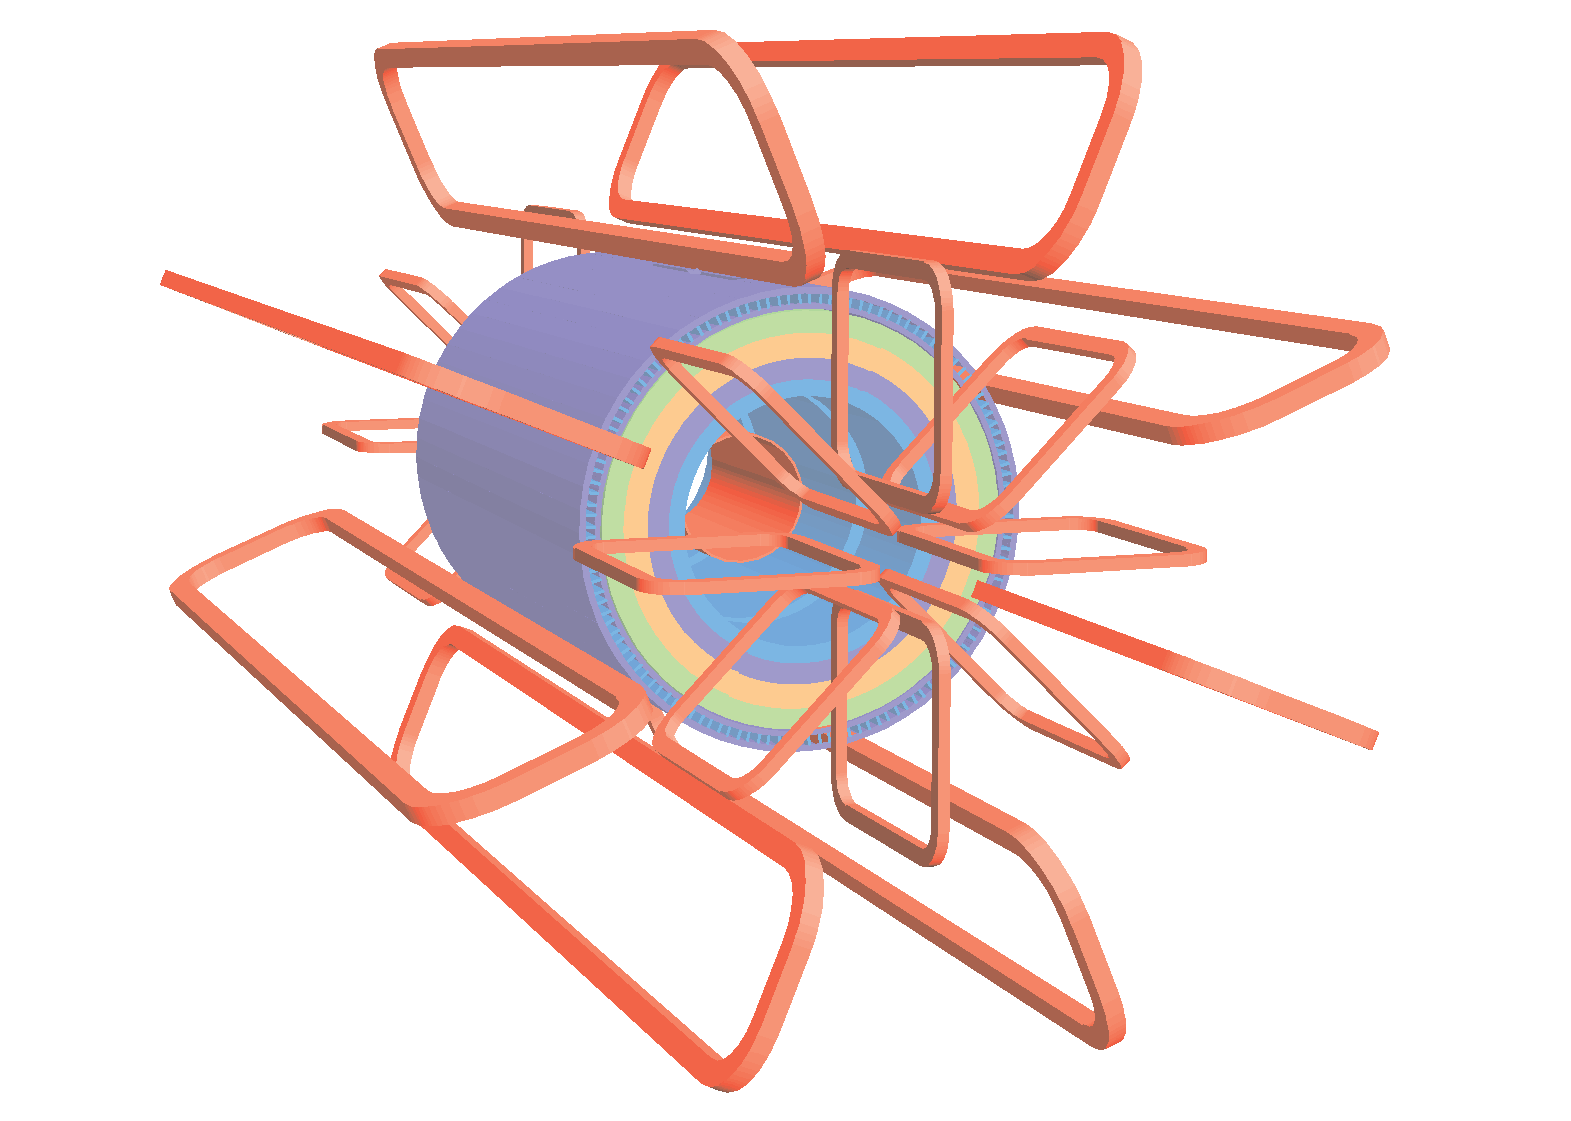
\includegraphics[width=.90\linewidth]{figures/atlas/ATLcoilGeom.eps}
\caption{The magnet system of the ATLAS detector. The inner cylinder shows the solenoid which gives a uniform magnetic field in the \ac{ID}. Outside of that are the barrel and endcap toroids, which provide a non-uniform magnetic field for the \ac{MS}.}
\label{fig:magnets}
\end{figure}
\end{centering}

The solenoid sits inside the calorimeter volume and provides a uniform 2T magnetic field to particles traveling through the \ac{ID}. This axial field causes the trajectories of charged particles to bend in the $x-y$ plane, and measurements of the curvature of these trajectories give the most accurate \pt measurement for many particles. 

Because the solenoid sits between the tracking system and the calorimeter, it is important that it interfere minimally with particles in order to allow the calorimeter to measure their full energies. The solenoid is placed inside the same vacuum chamber as the LAr calorimeter and is made of Al-stabilized NbTi superconductor with aluminum casing, giving it a total thickness of about 0.66 radiation lengths. 

The barrel toroid sits outside the calorimeters and provides the magnetic field for the barrel \ac{MS}, which varies from 0.2–2.5T. The endcap toroids have a magnetic field range of 0.2-3.5T. All three toroid magnets are made with Al-stabilized Nb/Ti/Cu superconducting coils supported by Al-alloy struts. 

The magnets are cooled with liquid helium, and take up to a month to be brought down to operating temperatures. All magnets have cold masses surrounding them to absorb heat in the event of a quench. 

The $B$-field resulting from this magnet system can be seen in \autoref{fig:bfield}. The plot on the left demonstrates the relatively constant field rate within the barrel which drops steeply at $|z|$=2. The right plot shows the field integral in the \acp{MDT} as a function of $|\eta|$, demonstrating the good coverage out to $|\eta|$<2.6 excluding a transition region between the barrel and endcap, where the field can can drop to around half its usual value. 

\begin{centering}
\begin{figure}[bth]
\myfloatalign
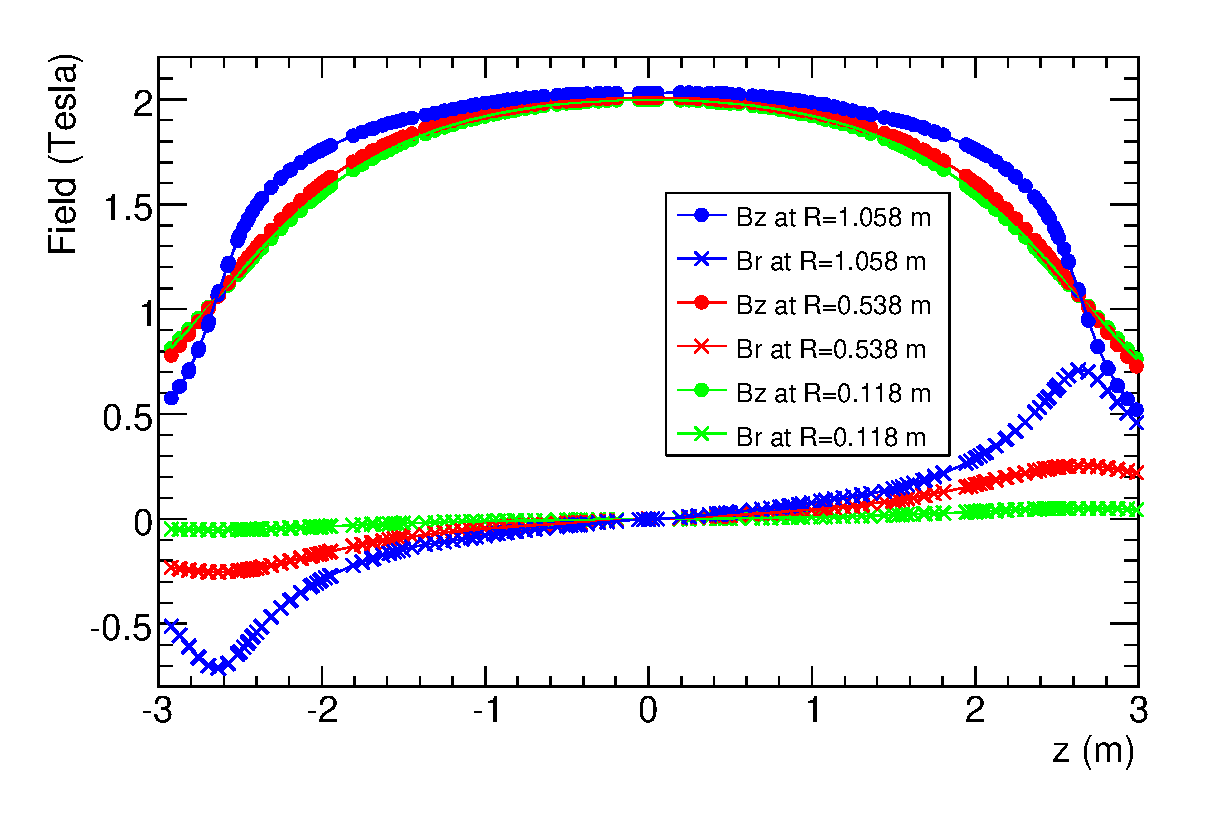
\includegraphics[width=.45\linewidth]{figures/atlas/solMeasB.eps}
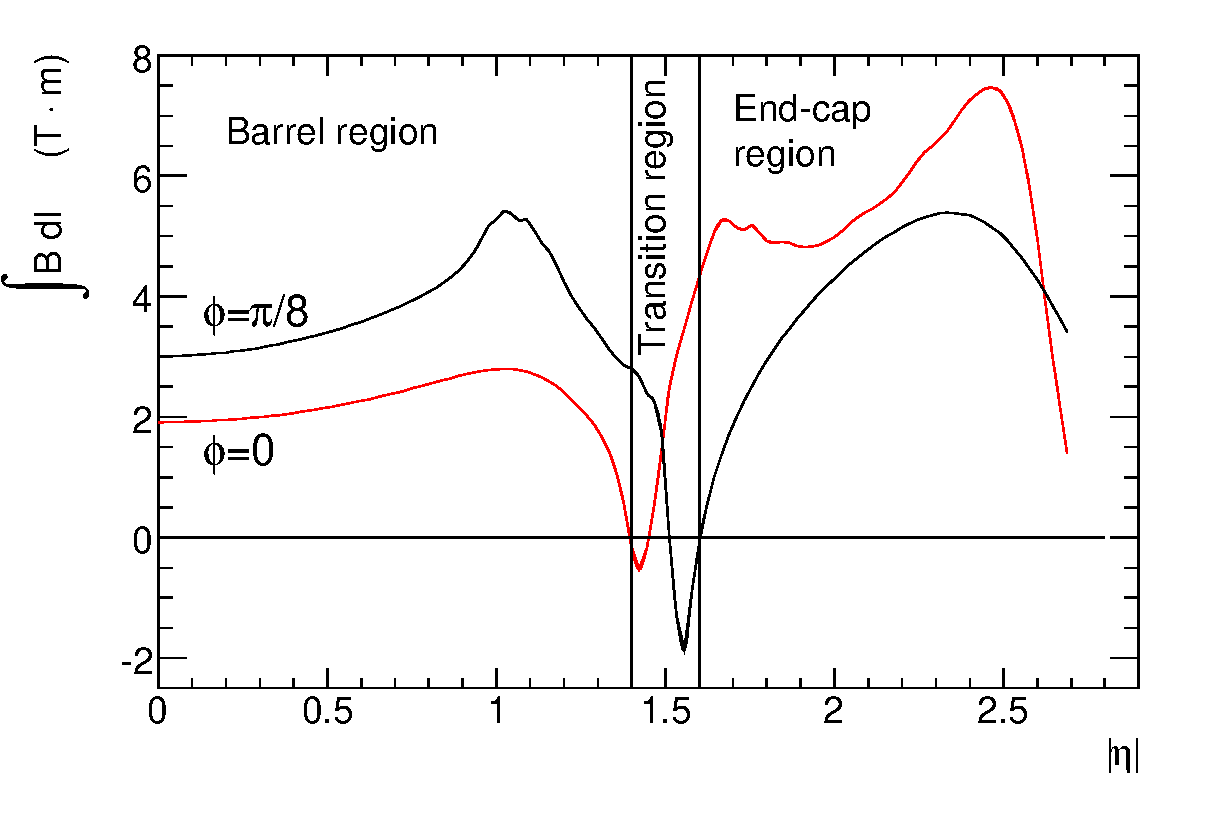
\includegraphics[width=.45\linewidth]{figures/atlas/IBdl.eps}
\caption{Plots of the magnetic field within the ATLAS detector. Left is the field (broken into its $R$ and $z$ components) as a function of $z$ for several different values of $R$. Right is the field integral through the \acp{MDT} as a function of $|\eta|$ for two different $\phi$ values. }
\label{fig:bfield}
\end{figure}
\end{centering}

\section{The Trigger System}
\label{sec:Trigger}

The \ac{LHC} provides proton bunch crossings every 25ns, and each of these events contains about one Mb of data, corresponding to 40Tb/s, a completely unmanageable amount of data. In addition to this concern, many of ATLAS's subdetectors like the pixel detector and \acp{MDT} take much longer than 25ns to read out, making keeping up with the bunch crossing rate impossible. To reduce the total data read out and allow for selective reading out of the slower detectors, a triggering system is used. 

The trigger system uses fast detectors to get a coarse picture of an event's topology, which is then compared to a trigger menu, which lists the types of events that are interesting enough to keep. Overall, the trigger system reduces the 40 million collisions a second to about 1000 to be fully read out from the ATLAS detector. 

This filtering of events is done in two steps: the \ac{L1} trigger is implemented in hardware and reduces the initial 40MHz to 100kHz, while the \ac{HLT} is implemented in software, further reducing the rate to 1kHz \cite{ATL-DAQ-PUB-2016-001}.The \ac{L1} trigger uses coarse granularity information from the fast read-out subdetectors: the calorimeters, the \acp{RPC} and \acp{TGC}. 

The coarse grained calorimeter information used for the \ac{L1} trigger decision is referred to as \ac{L1Calo} and uses information from all calorimeter systems. \ac{L1Calo} is responsible for all triggers excluding muons, meaning it must be capable of identifying a large number of different objects and event topologies, including high-\pt objects, large amounts of \met, andlarge amounts of hadronic energy.  
The outputs from the different calorimeters and the \ac{MS} can also be combined with a system called \ac{L1Topo}. Using this, triggers can require more complex topologies, and can suppress backgrounds from pileup by rejecting  


 % ATLAS
% Chapter 4b
\chapter{Object Reconstruction in the ATLAS Detector} % Chapter title
\label{ch:reconstruction} 

Object reconstruction is the computationally intensive process of interpreting the signals from the approximately 100 million read-out channels of the \ac{ATLAS} detector into a collection of particles and jets, the objects with which physics analysis can be performed. This process is complicated, and requires dedicated working groups in the \ac{ATLAS} experiment that optimize the understanding of each type of object. These groups must all collaborate to provide a full picture of the events in the detector. For each object type, candidate objects are reconstructed, and then an identification step is performed, which chooses which candidates will be used at the analysis level, based on a series of quality requirements.

%---------------------------------------------------------------------------------------

\section{Electrons}
\label{sec:reco_electrons}

Electrons are reconstructed through a combination of \ac{ID} and calorimeter measurements. They travel through the tracking system, leaving charge deposits in each layer, then are absorbed by the electromagnetic calorimeter. These two measurements work in conjunction to deliver high resolution measurements of electron momentum from low-\pt, where track curvature gives the most reliable measure of the electron's energy, to high-\pt, where the tracks are almost perfectly straight, but the calorimeter can still provide a reliable measurement. 

In the central region ($|\eta|<2.47$) of the \ac{ATLAS} detector, electron reconstruction begins with the identification of energy deposits in the electromagnetic calorimeter. The clusters of calorimeter cells are seeded by sliding longitudinal windows, which are measured in units of 0.025 in $\eta$ and $\phi$. 3$\times$5 unit windows are used, which require at least 2.5 \gev~in the window to form a seed \cite{Aad:2011mk}. 

These clusters are matched to \ac{ID} tracks by extrapolating each track to the middle layer of the calorimeter and identifying nearby clusters. If there are multiple tracks associated with a given cluster, tracks with silicon hits are preferentially chosen, and then the track with the smallest $\Delta R$ to the center of the cluster is selected. If a matching track is found, it is used to determine the likely direction of bremsstrahlung radiation in the calorimeter, and maximum distance to match a track to a cluster is expanded in the $\phi$ direction to account for this radiation. If no track is found, the cluster is rejected. 

The calorimeter clusters are then rebuilt in in larger windows, 3$\times$7 in the barrel and 5$\times$5 in the endcaps. An estimate of the energy is made by summing the measured calorimeter energy with estimates of the energy lost before the electron reached the calorimeter, energy outside of the cluster window, and energy not fully deposited in the calorimeter. These estimates are made with parametrized functions determined from a combination of \ac{MC} and measurements of energy loss determined with the presampler. 

The \pt of a central electron is determined though a combination of the calorimeter energy measurement and track measurements of the electron, while its $\eta$ and $\phi$ are taken from the track at its vertex. 

In the forward region, where no tracking is available, electron energy is determined more roughly. Calorimeter cells are formed into variable-sized clusters in regions of significant energy deposition, and the center of the cluster is used to determine angular coordinates of the electron. However, because these electrons have worse resolution in both their position and energy, they are rejected in this analysis. 

These reconstructed electron candidates' quality are then assessed based on an algorithm that uses multivariate analysis to assign a likelihood that a candidate is a true electron based on input from just under twenty different variables. These include track quality, hadronic leakage, cluster shape, and transition radiation, incorporating information from as many subdetectors as possible in its determination of the candidate's quality. Each variable is assigned a probability distribution function for true electrons and background processes, and they are collectively used to provide a \textit{likelihood} value which can be cut on. 

Three levels of identification, \texttt{Loose}, \texttt{Medium}, and \texttt{Tight}, are defined with different likelihood cuts, with electron candidates passing tighter identification levels always a subset of looser electrons. \autoref{fig:reco_el_eff} gives the efficiencies at each of these working points both for true electrons and for hadrons, which can be misidentified as electrons. Tighter working points have worse efficiencies, but lower misidentification rates for hadrons as well as photons. 

\begin{centering}
\begin{figure}[!hbt]
\myfloatalign
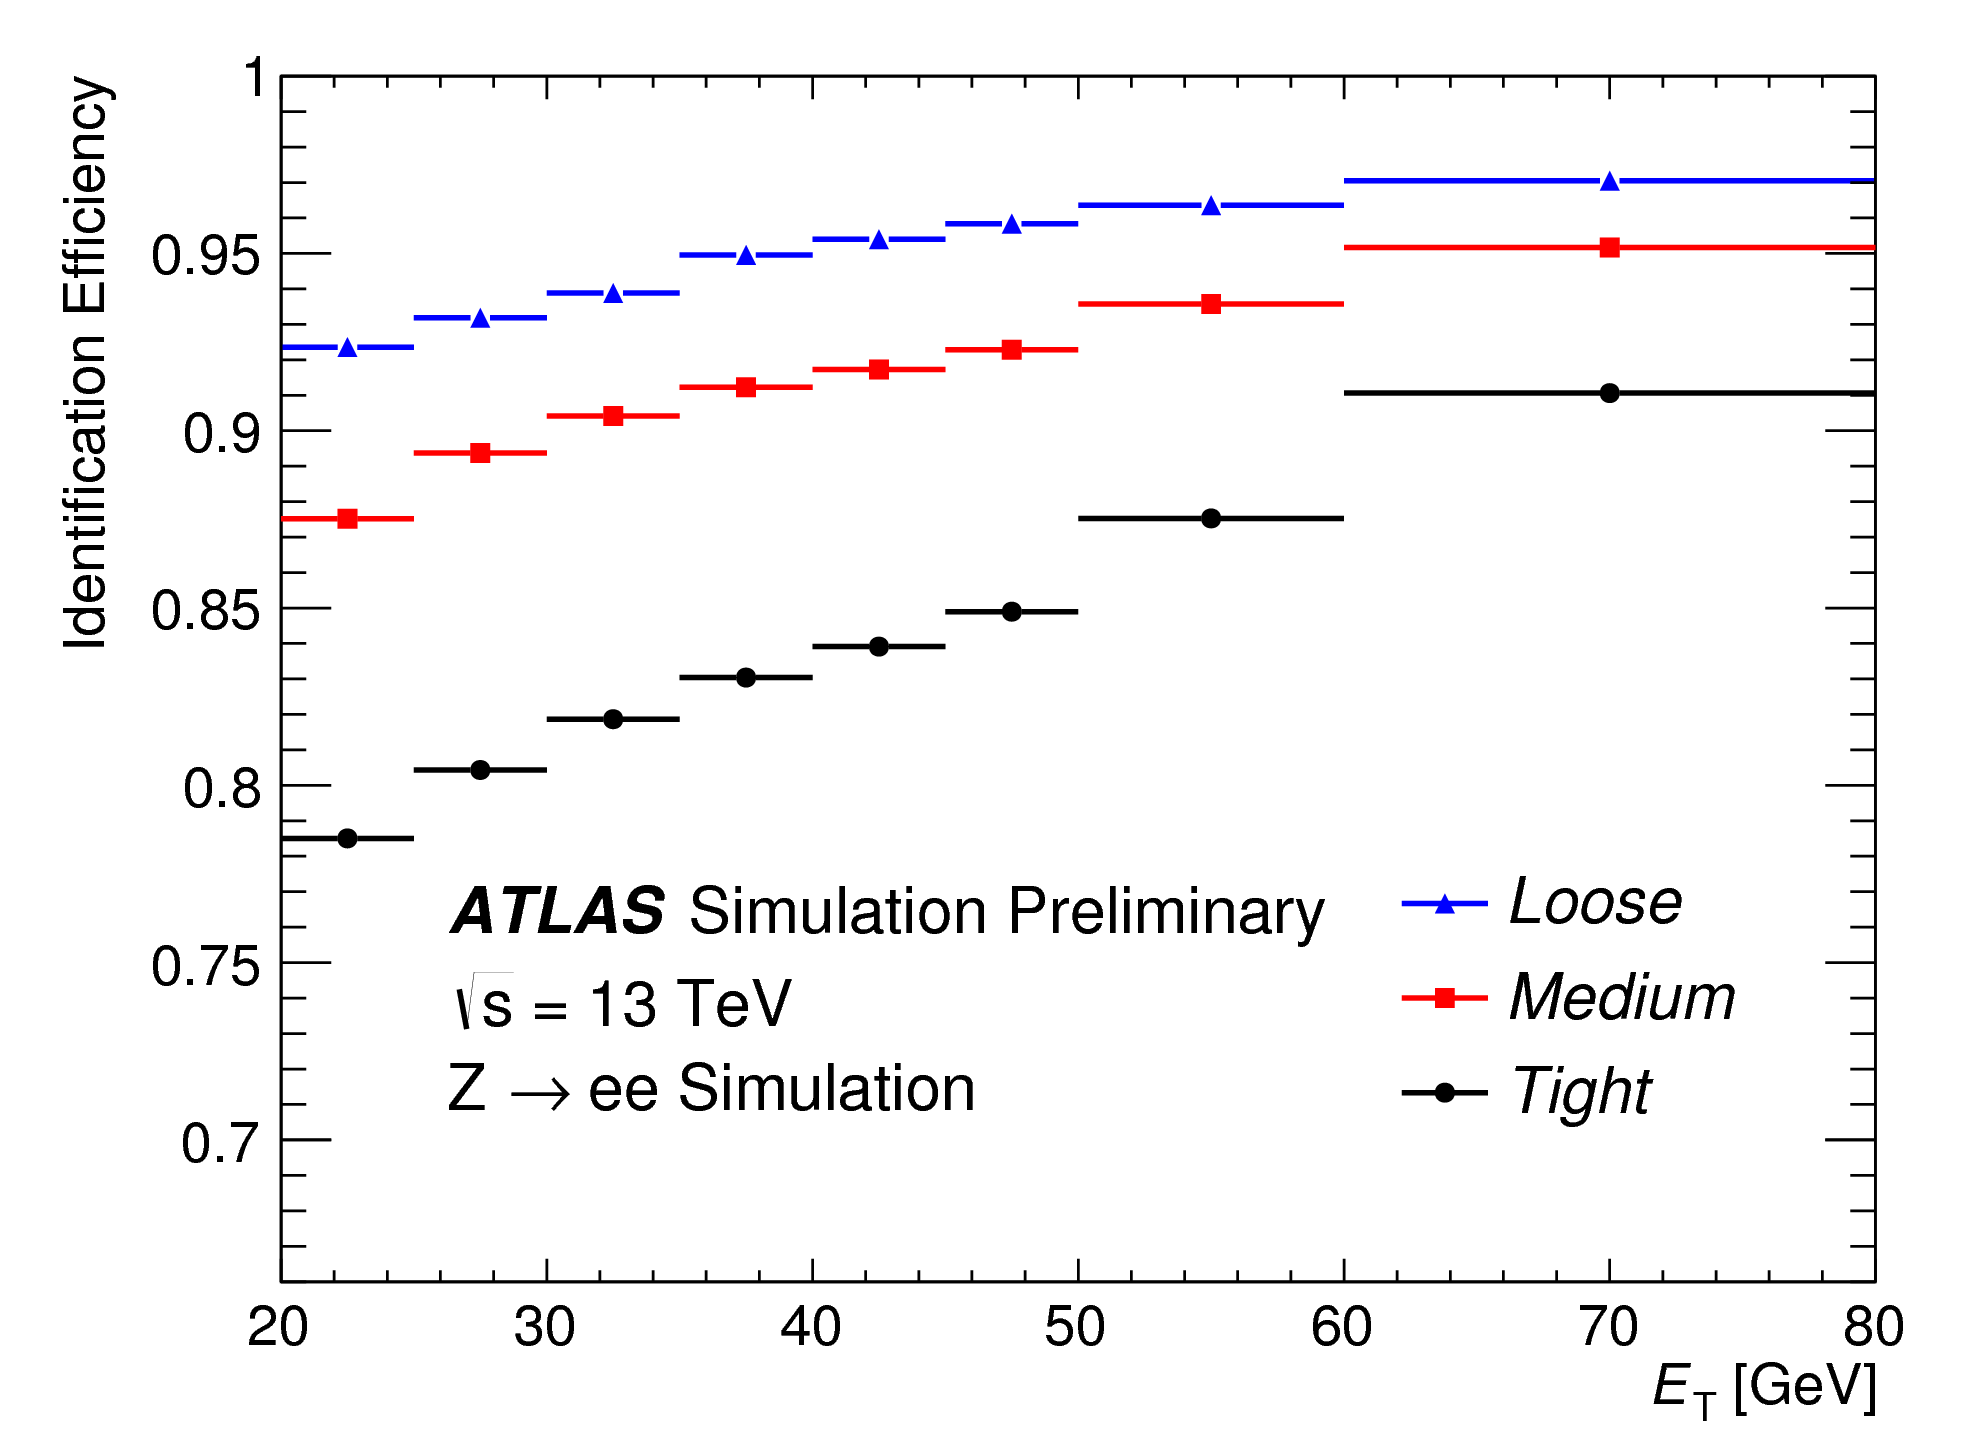
\includegraphics[width=.48\linewidth]{figures/reco/fig_01a.png}
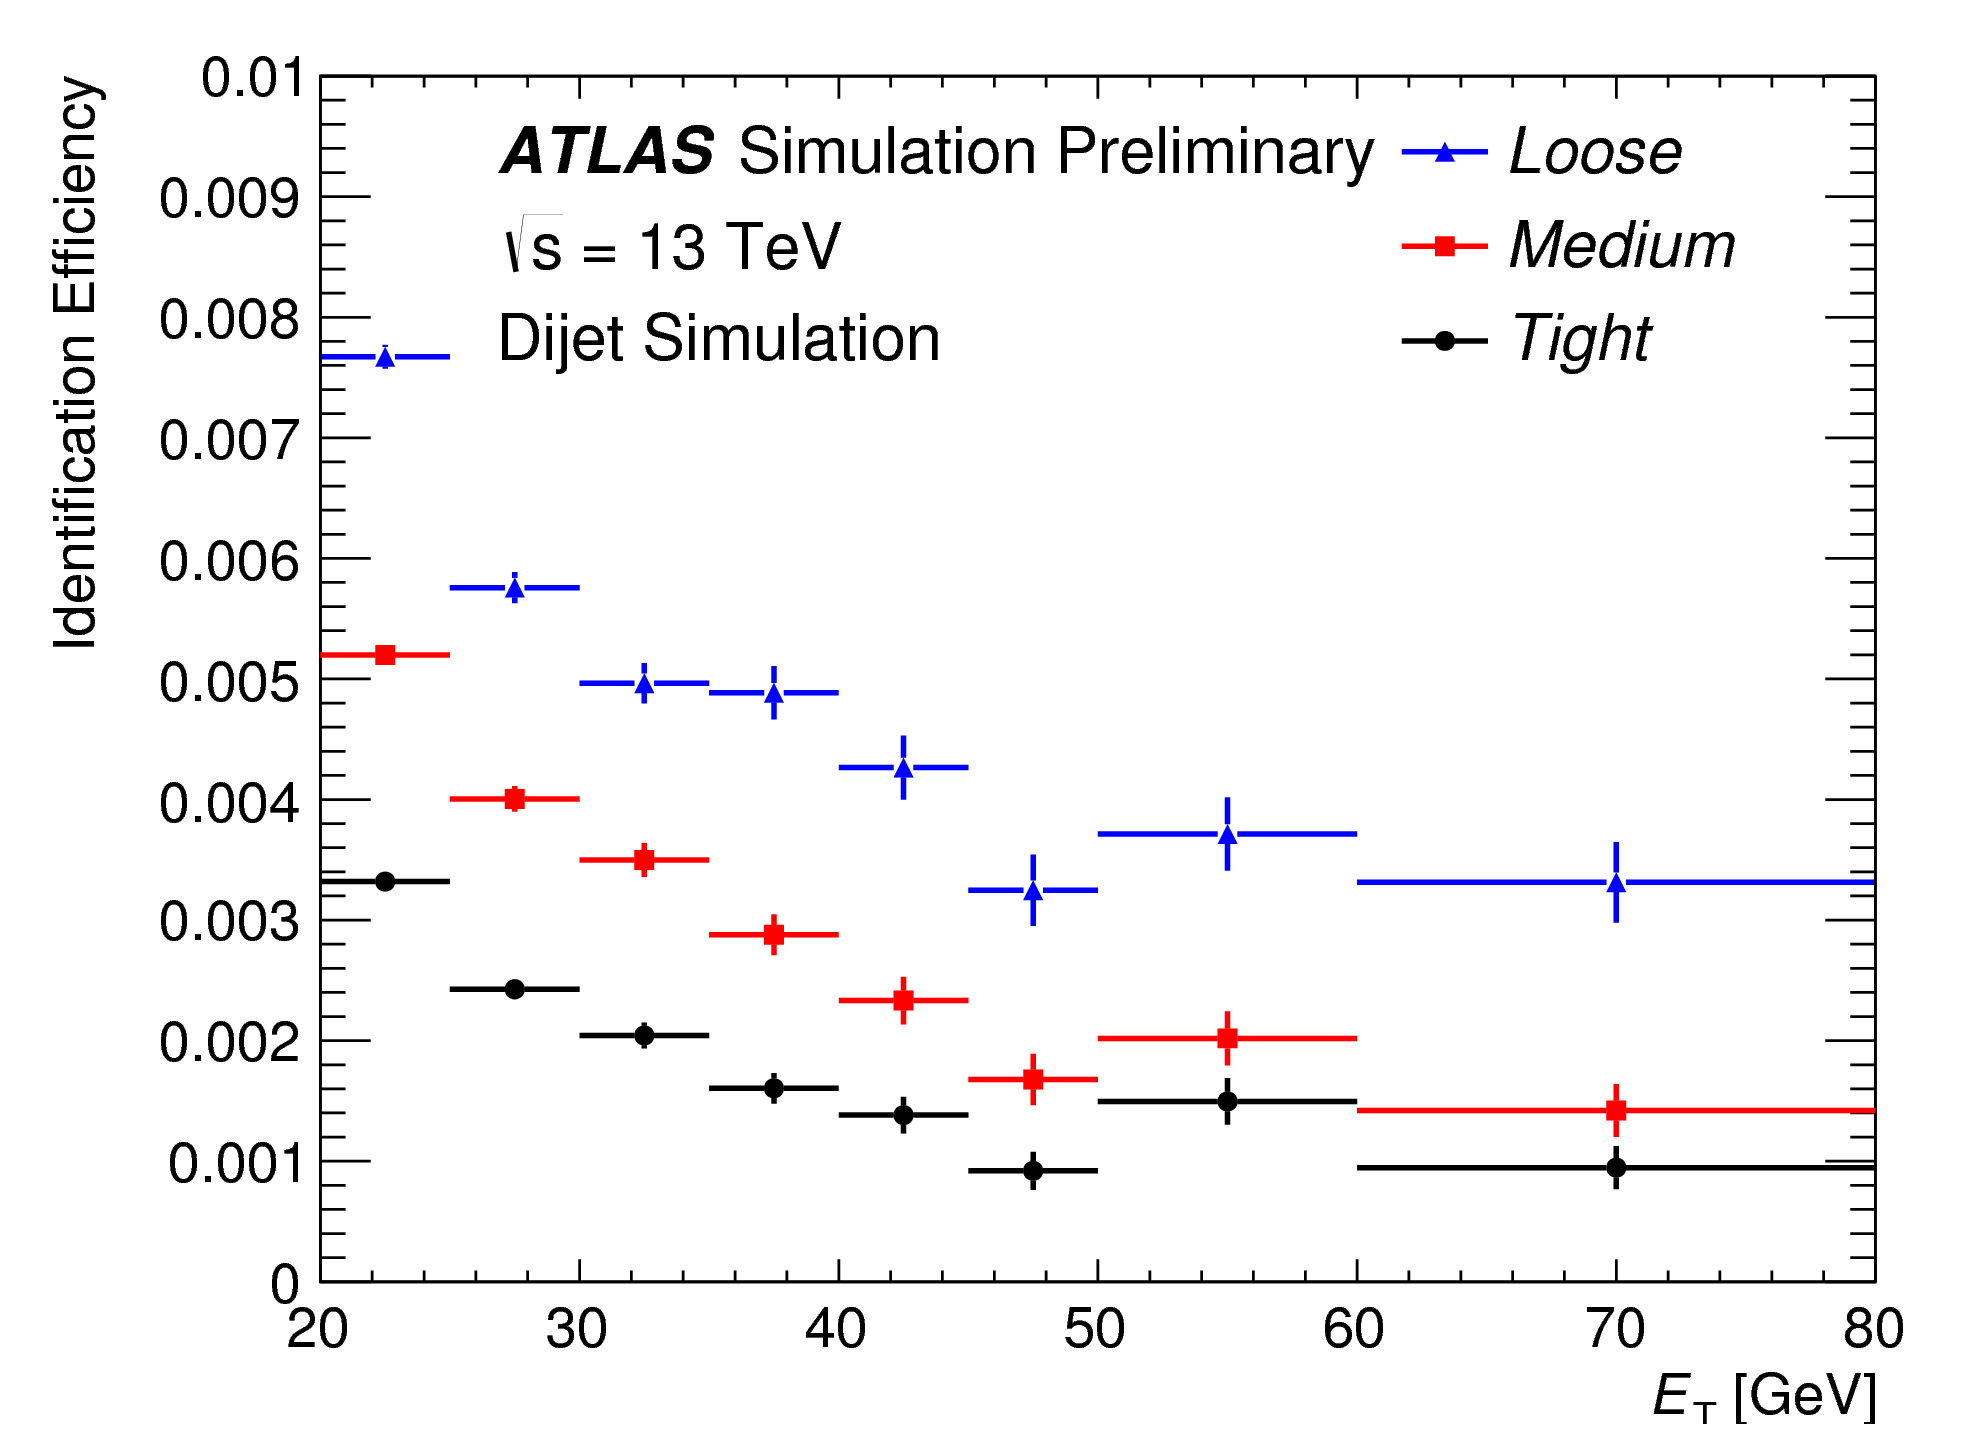
\includegraphics[width=.48\linewidth]{figures/reco/fig_01b.png}
\caption{ Identification efficiencies from \ac{MC} samples for \texttt{Loose}, \texttt{Medium}, and \texttt{Tight} working points. Left is the efficiency for identification of true electrons taken from $Z\rightarrow ee$ \ac{MC}, and right is the efficiency for mis-identification of jets as electrons taken from dijet \ac{MC} \cite{ATLAS-CONF-2016-024}.}
\label{fig:reco_el_eff}
\end{figure}
\end{centering}

\ac{MC} efficiencies can be compared to efficiencies measured in data to obtain a correction factor, which applied to \ac{MC} to better emulate the rates at which electrons are reconstructed and identified in data. \autoref{fig:reco_el_sf} shows a comparison of the combined reconstruction and identification efficiencies in data and \ac{MC}, with the resulting correction factors also displayed as the ratio. This analysis uses the \texttt{Medium} working point, which has correction factors ranging between 2 and 10\%. 

\begin{centering}
\begin{figure}[!hbt]
\myfloatalign
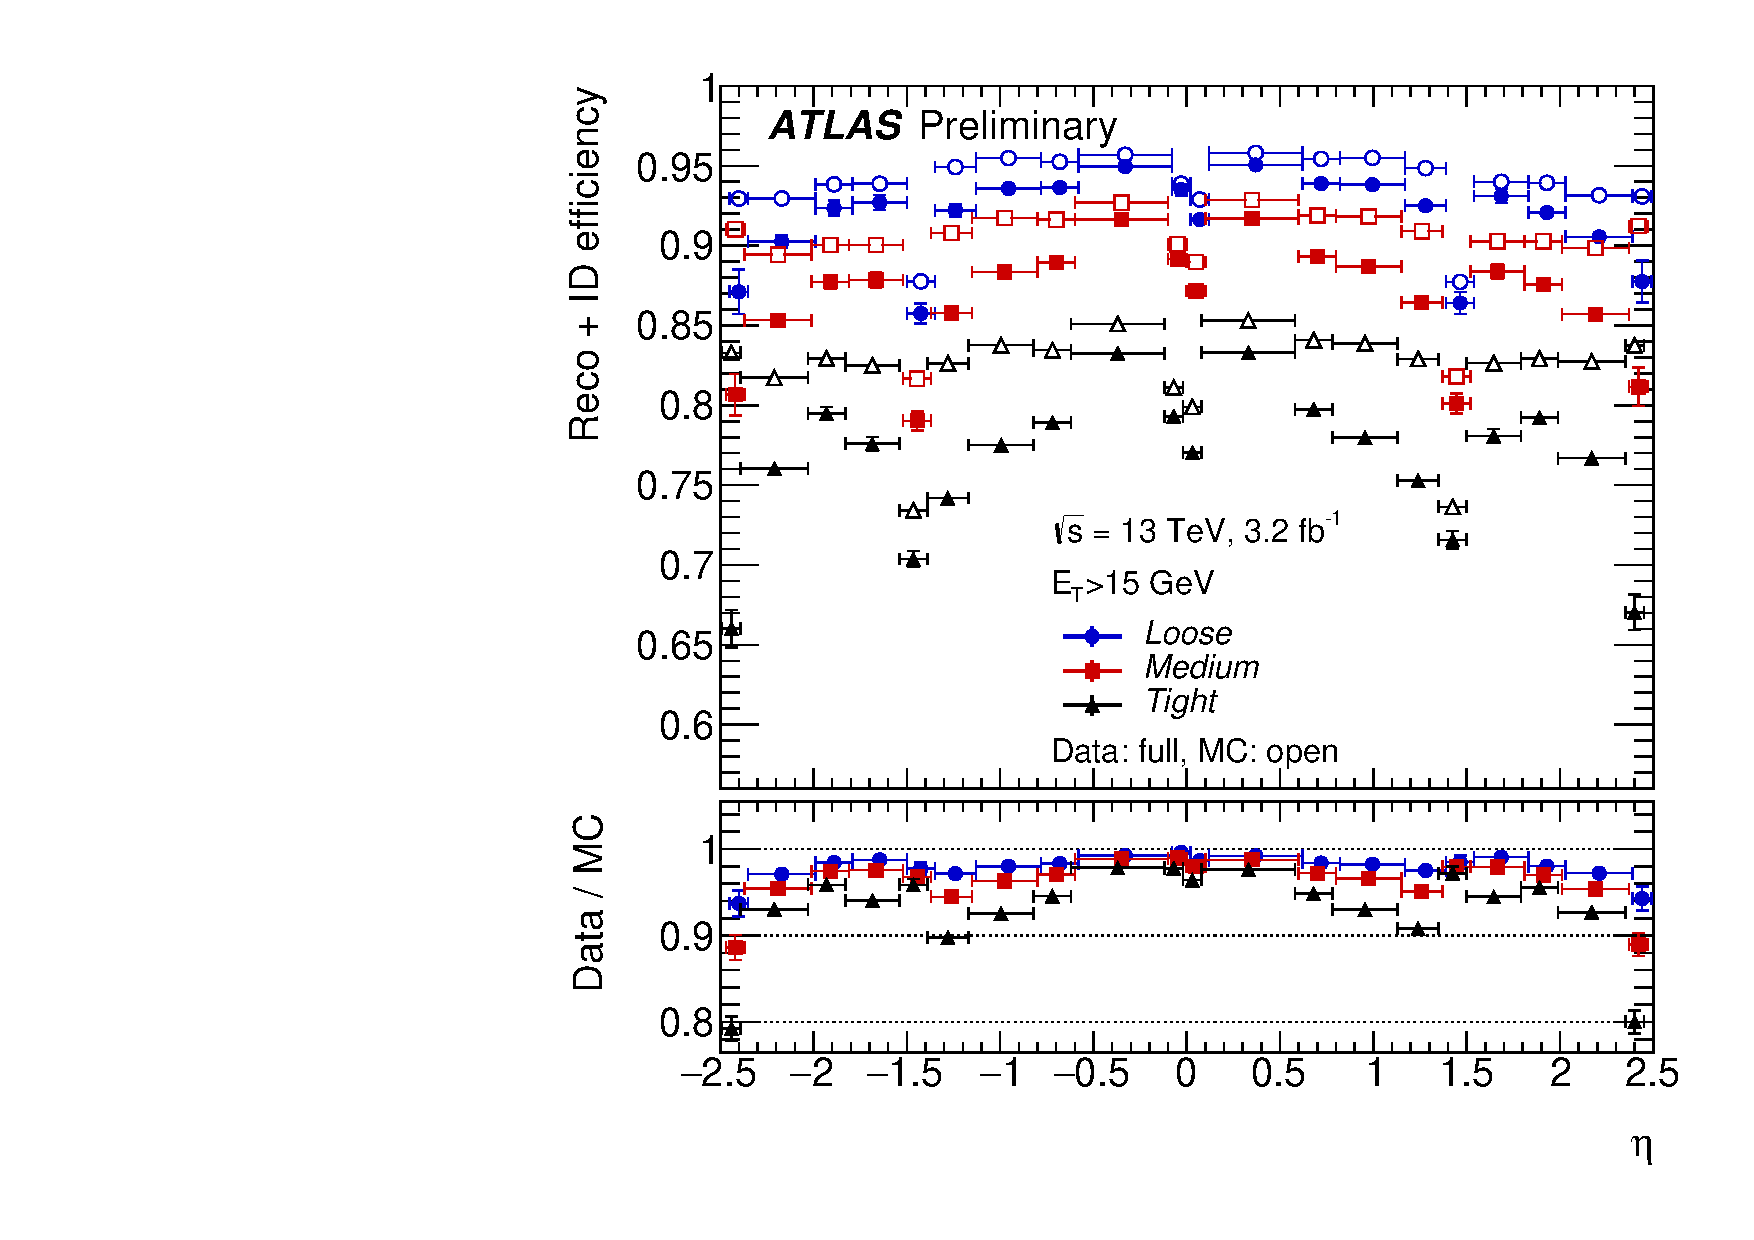
\includegraphics[width=.90\linewidth]{figures/reco/fig_14b.pdf}
\caption{ Combined electron reconstruction and identification efficiencies measured as a function of $\eta$ for data (using the tag-and-probe method on $Z\rightarrow ee$ events) and $Z\rightarrow ee$ \ac{MC}. Distributions include electrons with \et > 15 \gev. \cite{ATLAS-CONF-2016-024}.}
\label{fig:reco_el_sf}
\end{figure}
\end{centering}

Requirements are also made on electron \textit{isolation}, which quantifies the amount of energy deposited near the electron according calorimeter and track measurements. Isolation variables are primarily used to reject non-prompt leptons, leptons which aren't produced by the initial hard scattering of the $pp$ collision. These can be produced by heavy flavor hadron decays and converted photons, as well as misidentified hadrons. Cuts are made on the amount of nearby calorimetric energy and sum of the \pt of any nearby tracks relative to the electron's energy, forming a series of working points. Working points are created based on their efficiency, including \texttt{Tight} and \texttt{Loose} working points, which operate at 95 and 98\% efficiency respectively. The most effective working points target different efficiencies as a function of \pt, with higher efficiencies possible at high \pt due to reduced fake backgrounds. There are two such working points, \texttt{Gradient} and \texttt{GradientLoose}. They each have a 99\% efficiency for electrons with \pt > 60 \gev, but 90 and 95\% efficiencies at 25 \gev. To recover the largest possible fraction of electrons, this analysis uses \texttt{GradientLoose}.

\section{Photons}
\label{sec:reco_photons}

The reconstruction of photons is performed in parallel to electron reconstruction. Seed clustering is performed, and tracks are matched to these clusters, as in the case of the electron reconstruction described in \autoref{sec:reco_electrons}. 

Photons can be converted to electron-positron pairs in the \ac{ID}, leaving a pair of tracks, or they can pass through without conversion, leaving no tracks behind. As a consequence, calorimeter clusters resulting from photons can have no tracks associated with them, two tracks, or one track, in the case that one of the conversion tracks is not reconstructed. The reconstruction software attempts to identify all these scenarios and differentiate these clusters from electron and hadron deposits \cite{1606.01813}.

Two-track clusters are required to consist of two oppositely charged tracks that emerge from a conversion vertex running parallel to one another. A likelihood that these tracks are from electrons is determined using the high threshold hits in the \ac{TRT}, and quality requirements are made on the tracks using this likelihood. For tracks with silicon hits, a loose likelihood requirement of 10\% is made, while tracks without silicon hits are required to have at least 80\% likelihood. The tracks are then fit to determine the conversion vertex, and quality cuts are made, such as requiring that conversion vertices within the silicon volume correspond to tracks with silicon hits. 

Single track clusters occur most often from conversions in the outermost layers of the \ac{ID}, and are more difficult to reconstruct. Tracks are typically lost because an electron or positron resulting from the conversion has a \pt too low to be reconstructed, or because the two tracks are so close together that they're identified as a single track. The single track is required to have at least a 95\% electron likelihood from \ac{TRT} hits, and must not have a hit in the innermost layer of the pixel detector. The conversion vertex is defined as the first hit of the single track. 

The tracks associated with these conversion vertices are extrapolated to the calorimeter and matched to cluster, except in the case that there are two tracks that differ substantially in their \pt measurements, in which case the position of the conversion vertex is used for extrapolation to the calorimeter, assuming a straight-line trajectory. If multiple vertices are matched to a single cluster, preference is given to vertices with double tracks, silicon hits, and finally to tracks closest to the interaction point. 

Any cluster with neither a conversion vertex or a track associated with it is identified as an unconverted photon. Clusters associated with both electrons and photons are assigned to one or the other based on their properties. Clusters are preferentially identified as photons in the case that they are matched to a conversion vertex in which at least one track is associated with both the vertex and the cluster, or if the associated tracks have a \pt smaller than the cluster's \pt. $E/p$, the ratio of the cluster and track energy measurements, can also be used to differentiate electrons and photons. Electron candidates are instead reconstructed as photons if they have $E/p>10$ or if the track matched to the electron has \pt below 2 \gev. 


Photon energy is determined in a 3$\times$5 (3$\times$7) window for unconverted (converted) photons in the barrel, where the window is expanded to compensate for the increased spread of energy from the conversion products. In the endcap, the 5$\times$5 window is used in all cases. Like the electrons, the calibration of the photon's energy accounts for energy loss before the calorimeter, as well as energy deposited outside the cell and beyond the electromagnetic calorimeter.

Photon identification is performed in the range $|\eta|<2.37$ using a series of cuts on the shape of the shower in the electromagnetic calorimeter, as well as the amount of additional energy deposited in the hadronic calorimeter. Photons in the the so called \textit{crack} region of the calorimeter ($1.37<|\eta|<1.52$), where a discontinuity prevents accurate assessment of photon energy, are rejected. The photon identification has only one working point, called \texttt{Tight}, which has an identification efficiency of 53–64\%(47–61\%) for unconverted (converted) photons with \et = 10 \gev~and 88–92\% (96–98\%) for photons with \et $\geq$ 100 \gev~\cite{ATL-PHYS-PUB-2016-014}. Efficincies as a function of \pt measured in the 2016 data and compared to \ac{MC} can be seen in \autoref{fig:reco_photon_eff}.

\begin{centering}
\begin{figure}[!hbt]
\myfloatalign
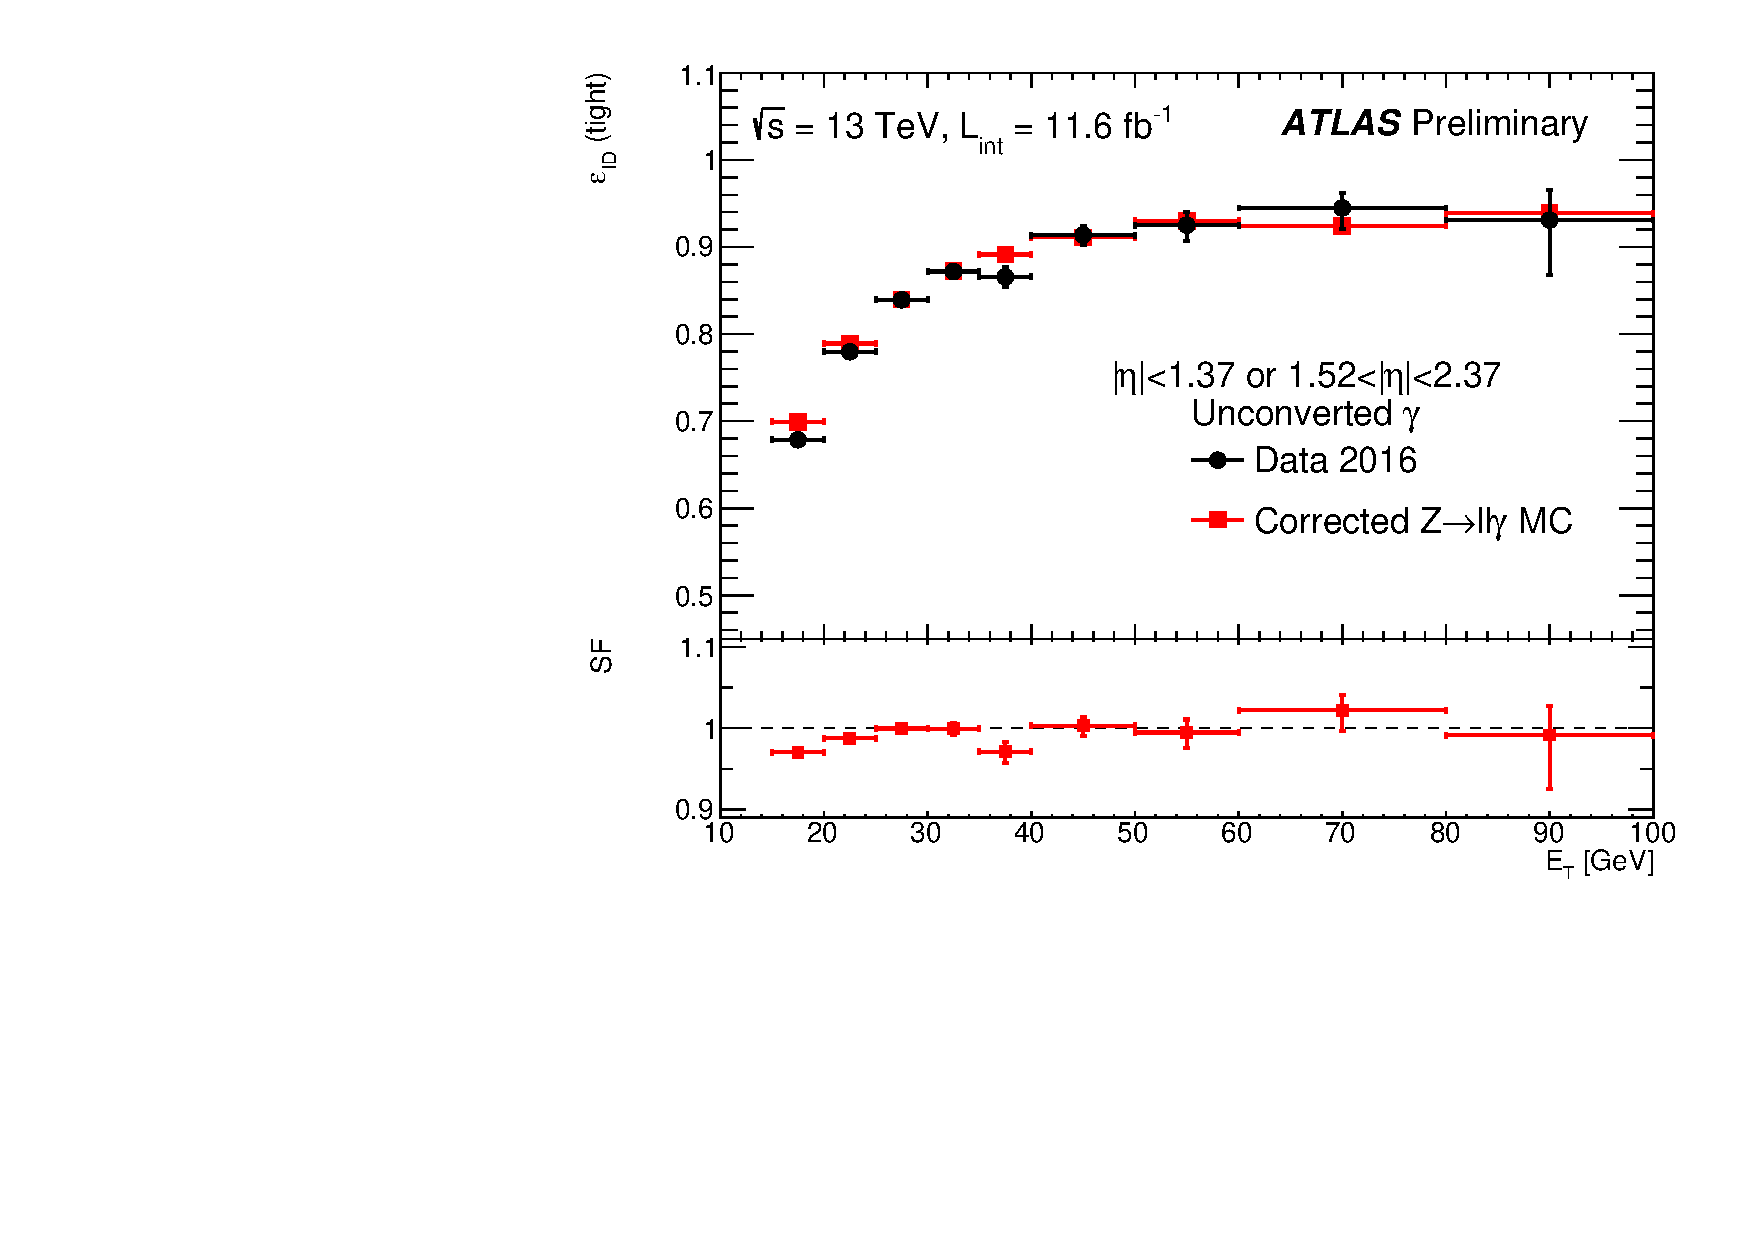
\includegraphics[width=.48\linewidth]{figures/reco/photon_fig_01.pdf}
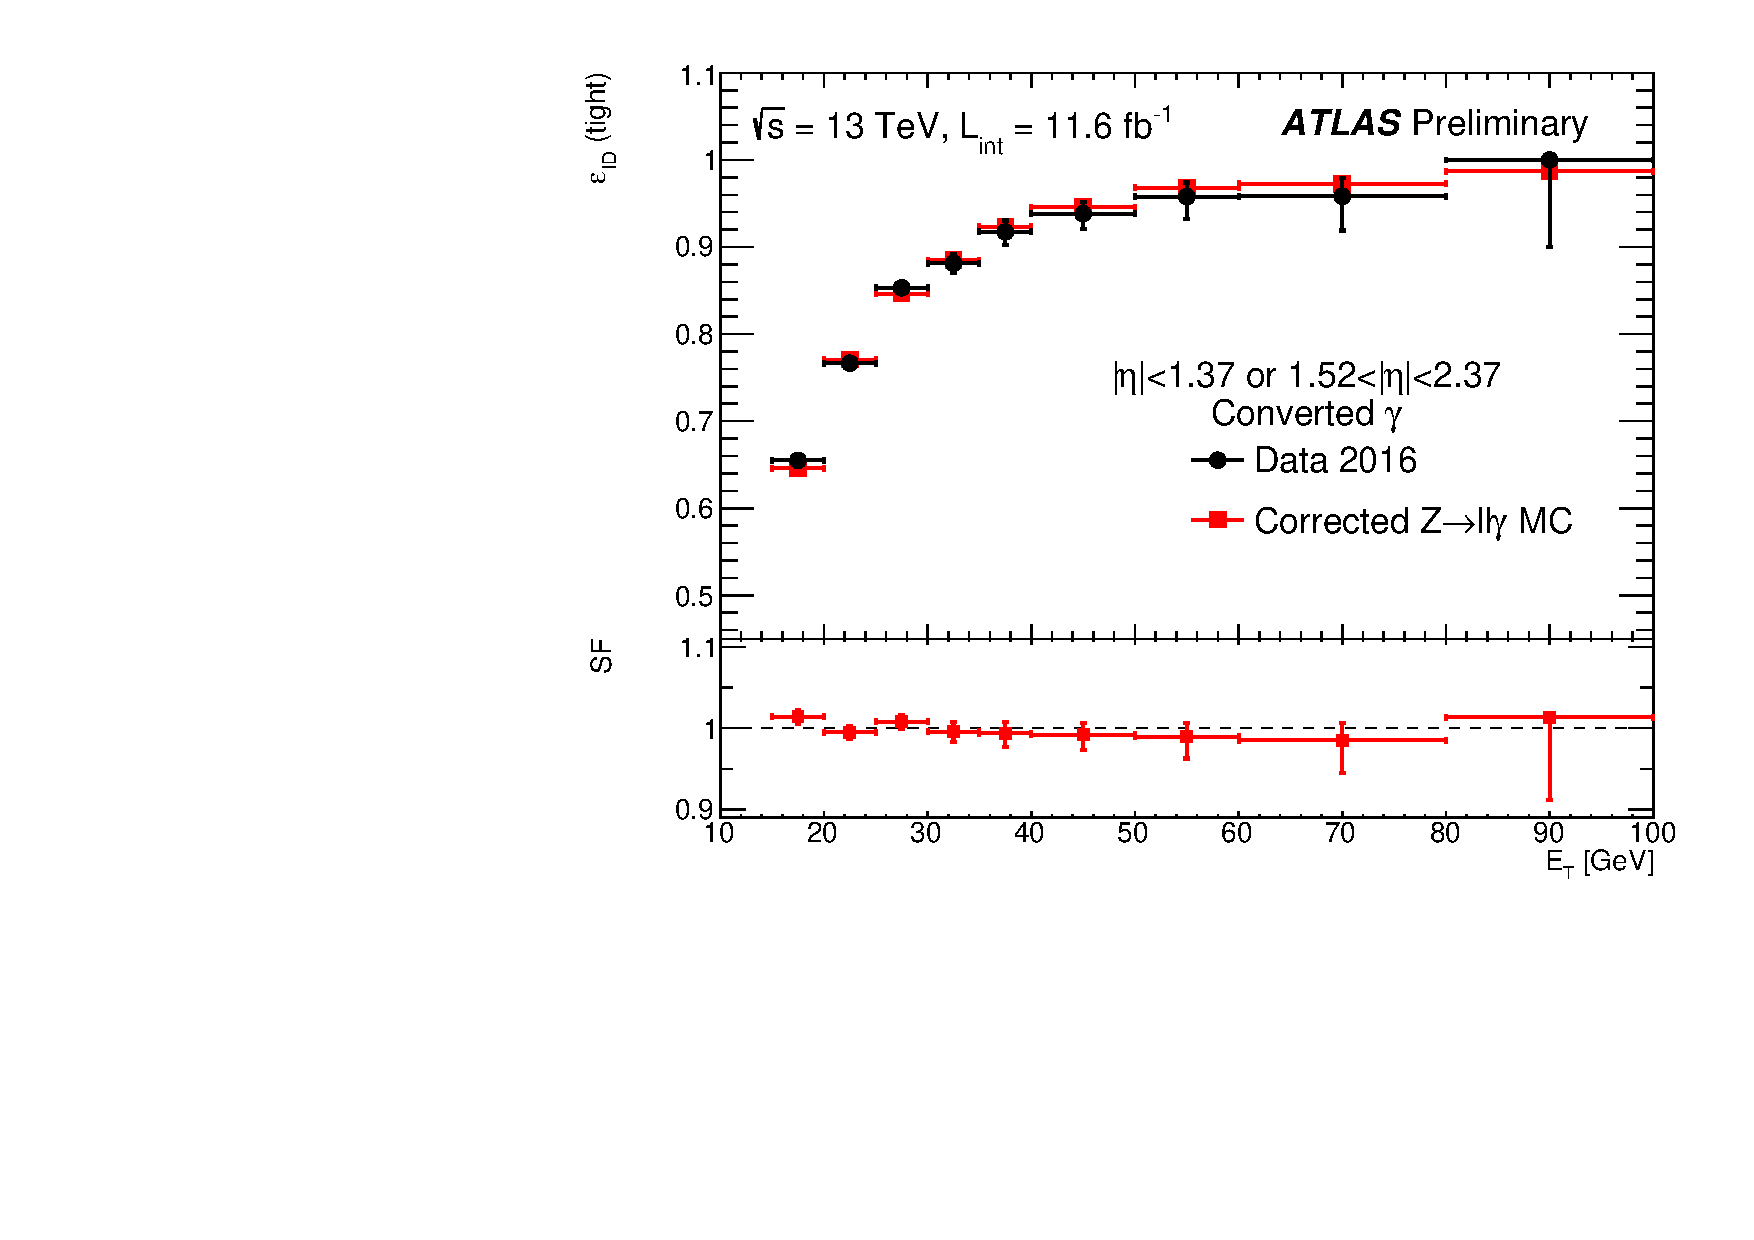
\includegraphics[width=.48\linewidth]{figures/reco/photon_fig_02.pdf}
\caption{ Comparison of \texttt{Tight} identification efficiency measurements from data and $Z\rightarrow \ell\ell\gamma$ \ac{MC} for unconverted (left) and converted (right) photons, with an inclusive $\eta$ selection. The bottom of each figure shows the ratio of data and \ac{MC} efficiencies. \cite{EGAM-2016-003}.}
\label{fig:reco_photon_eff}
\end{figure}
\end{centering}

Photon isolation, like electron isolation, can be determined as the combination of nearby calorimeter deposits and tracks. Fixed cuts on the isolation as a fraction of photon energy is typically used. A working point called \texttt{FixedCutTight} reconstructs the amount of calorimeter energy (excluding that of the photon) in a cone of $\Delta R  = 0.4$ around the photon and the amount of energy from the sum of track \pt in a cone of $\Delta R = 0.2$, including only tracks associated with the primary vertex. Defined relative to the photon's \pt, this working point includes photons with calorimetric isolation less than 0.022 \pt + 2.45 \gev~and track isolation less than 0.05 \pt \cite{isolation}. 

\section{Muons}
\label{sec:reco_muons}

Muon reconstruction is performed independently in the \ac{ID} and the \ac{MS}, then the two measurements are combined when consistent tracks are found in each system \cite{1603.05598}. The \ac{ID} reconstruction is performed using the tracking algorithms described in \autoref{sec:tracking}, and includes tracks with $|\eta|<2.5$. 

The \ac{MS} track reconstruction is performed in the $|\eta|<2.7$ range and begins with a search in each muon chamber for patterns of hits consistent with a track, called \textit{segments}. The \ac{MDT} chamber hits are fit to a straight line, and nearby \ac{RPC} and \ac{TGC} chambers provide the coordinate orthogonal to the magnetic curvature for these hits. Segments are also built in the \ac{CSC}, where they are required to be loosely consistent with a track originating from the interaction point. 

These segments are then fit together, starting from the middle layers of the \ac{MS}, with track quality requirements on the resulting combinations based on the $\chi^2$ of the fits. Tracks must have at least two segments, except in the transition region between the barrel and endcap, where a single segment can qualify as a track. Segments are allowed to be shared between multiple tracks in the initial reconstruction, but after the combination, tracks with shared segments and poor $\chi^2$ are removed.    

These \ac{MS} tracks are then combined with measurements from the \ac{ID} and calorimeters. The best quality muons are combined muons, which have \ac{ID} and \ac{MS} tracks associated to them, the hits of which are re-fit to form a combined track. \ac{MS} hits can be added or removed at this stage based on their consistency with the new track. Lower quality muon candidates are also defined. Extrapolated muons have only \ac{MS} tracks and their trajectories are required to be consistent with the interaction point. Calorimeter-tagged muons combine an \ac{ID} track with a calorimeter deposit consistent with a muon, while segment-tagged muons combine an \ac{ID} track with a segment in the \ac{MS}. Muons with shared \ac{ID} tracks are not allowed, with preference given to combined muons, then calorimeter-tagged muons, and lastly segment-tagged muons. 

There are four muon identification working points for muons: \texttt{Loose}, \texttt{Medium}, \texttt{Tight}, and \texttt{High-p$_\texttt{T}$}. These working points all have different efficiencies for the identification of muons, balanced against the mis-identification of hadrons. One of the key variables for their discrimination is $q/p$ significance, which quantifies the consistency between the \ac{ID} and \ac{MS} measurements of momentum. The $\chi^2$ of the combined fit is also an important discriminator. 

The \texttt{Loose}, \texttt{Medium}, and \texttt{Tight} selections are inclusive, with all \texttt{Tight} muons passing the \texttt{Medium} requirements, and \texttt{Medium} muons passing the \texttt{Loose} requirements. %The \texttt{Loose} requirement includes all types of reconstructed muons, but allows muons without \ac{MS} tracks (calorimeter- and segment-tagged muons) only in the $\eta<0.1$ range where there is a gap in the \ac{MS} coverage to accommodate cabling for the calorimeter system. 
The \texttt{Medium} working point includes only combined and extrapolated muons, and is the default for most \ac{ATLAS} analyses, including this one. Extrapolated muons are allowed only outside the \ac{ID} tracking system ($|\eta|>2.5$) for this working point, but this region is excluded by this analysis because of the decreased efficiency and larger \pt resolution of these muons. As a consequence, this analysis uses only combined muons. For these muons, the \texttt{Medium} working point requires at least three hits in at least two \ac{MDT} layers (except in the $\eta<0.1$ region) and a $q/p$ significance cut is made to reduce backgrounds. Due to the lack of coverage at low $\eta$, there is a drop in efficiency in this region, as shown in \autoref{fig:reco_muon_eta}. %The \texttt{Tight} working point additionally cuts on $\chi^2$ and makes further requirements on the consistency between \ac{ID} and \ac{MS} \pt measurements. 

\begin{centering}
\begin{figure}[!hbt]
\myfloatalign
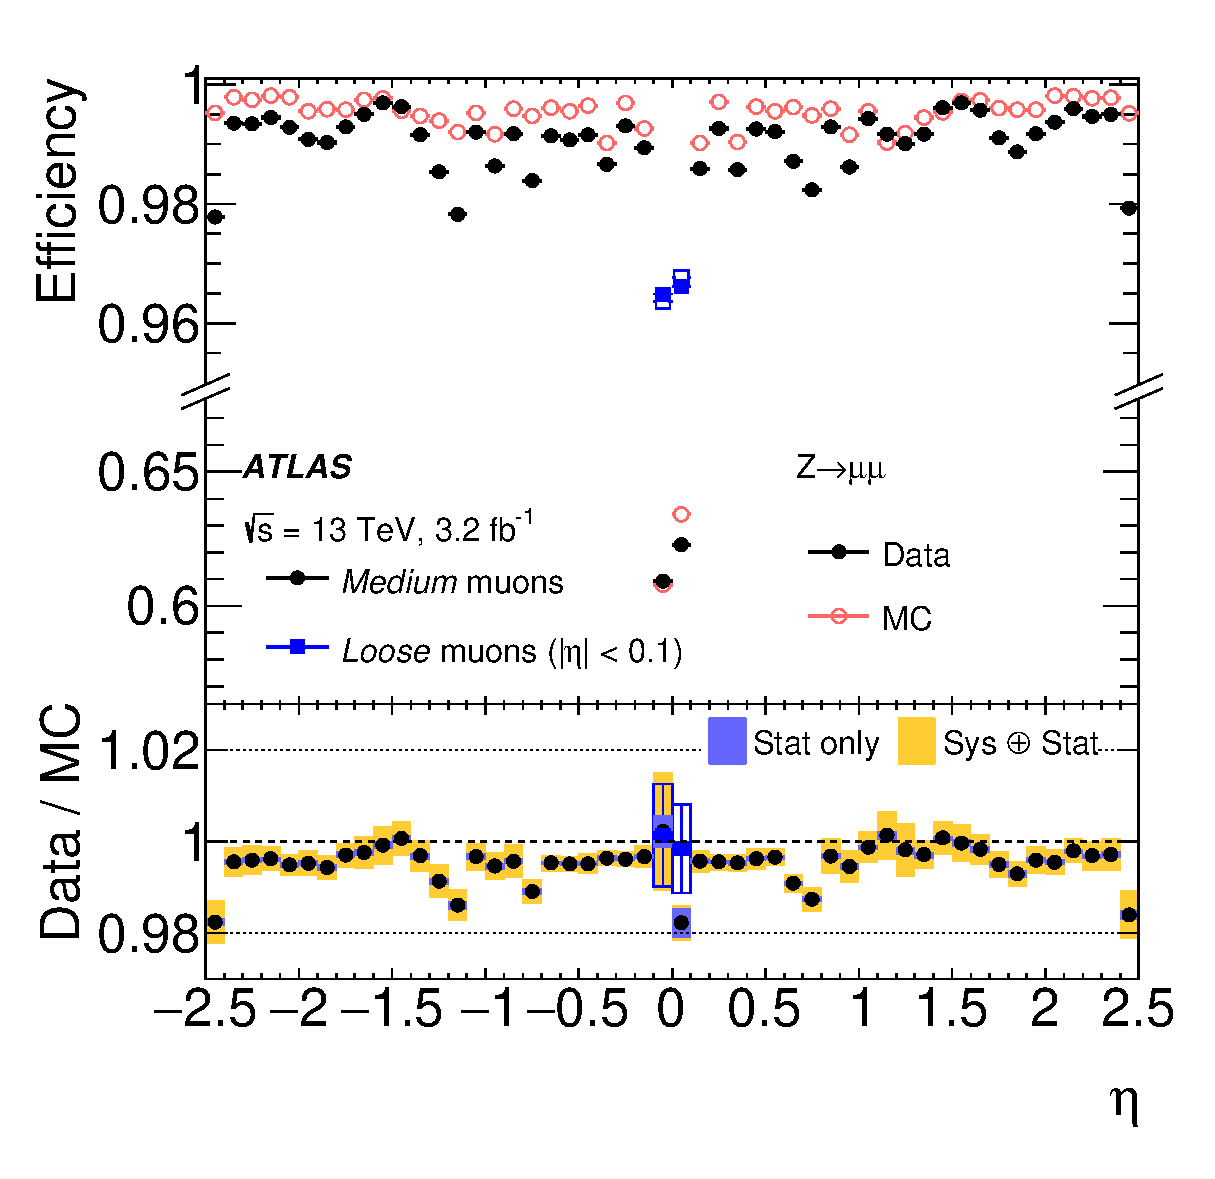
\includegraphics[width=.9\linewidth]{figures/reco/fig_03a.eps}
\caption{Muon reconstruction efficiency for the \texttt{Medium} and \texttt{Loose} working points measured with $Z\rightarrow\mu\mu$ events in data and in \ac{MC} as a function of $\eta$. The ratio between the two is shown at the bottom. The \texttt{Loose} working point efficiency is shown only at  small $|\eta|$, where the loosened requirements cause the largest difference from the \texttt{Medium} working point \cite{1603.05598}. }
\label{fig:reco_muon_eta}
\end{figure}
\end{centering}

The \texttt{High-p$_\texttt{T}$} working point is designed to minimize the resolution for high-\pt muons, at the cost of lower efficiencies. Muons passing the \texttt{High-p$_\texttt{T}$} requirements must have at least three \ac{MDT} hits in three layers, which decreases efficiency but gives greatly improved \pt resolution. In addition, some regions of the \ac{MS} with poor alignment are vetoed to cut down on mismeasurement. Compared to the default working point these muons have much lower efficiency: 78\% (90\%) for \texttt{High-p$_\texttt{T}$} muons compared to 96\% (96\%) for \texttt{Medium} in the \pt range of 4-20 \gev~(20-100 \gev). The efficiency as a function of $\eta$ for this working point can be seen in \autoref{fig:reco_muon_eta_highpt}, where the efficiency loss due to the of vetoing of some chambers is especially apparent. Mismodeling of the alignment and the specificity of the momentum resolution cuts cause a large discrepancy between data and \ac{MC} efficiencies, resulting in scale factors that differ from unity by as much as 10\%. This working point was considered for this analysis, where mismeasurement of muons increases \ac{SM} backgrounds, but ultimately the \texttt{Medium} working point was chosen for its superior efficiency and better modeling in \ac{MC}.

\begin{centering}
\begin{figure}[!hbt]
\myfloatalign
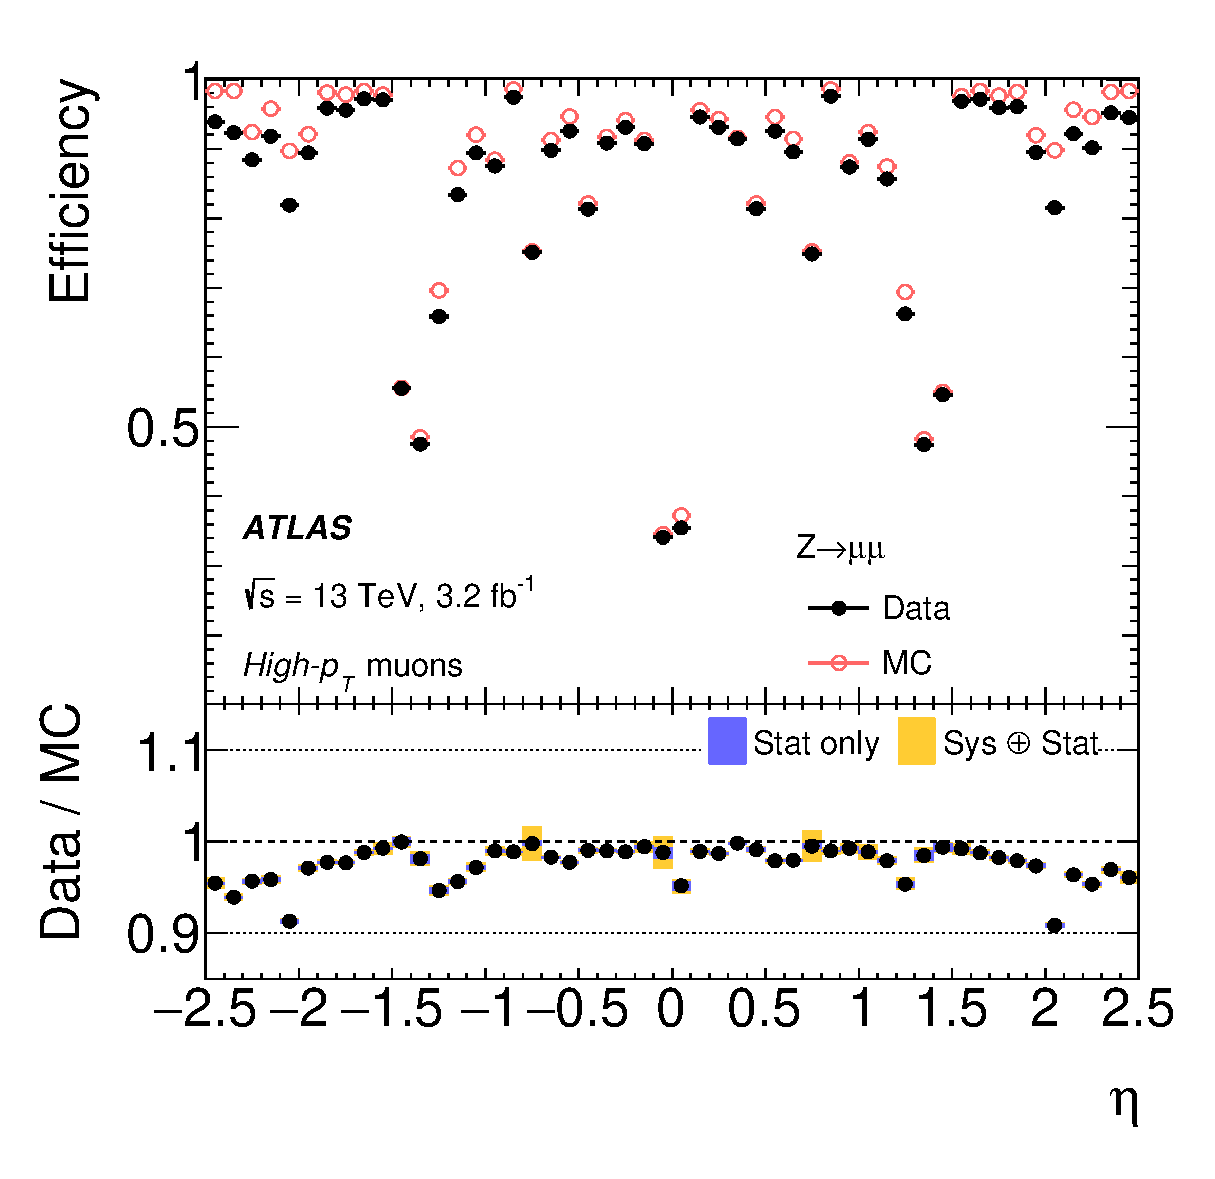
\includegraphics[width=.9\linewidth]{figures/reco/fig_03c.eps}
\caption{Muon reconstruction efficiency for the \texttt{High-p$_\texttt{T}$} working point measured with $Z\rightarrow\mu\mu$ events in data and in \ac{MC} as a function of $\eta$. The ratio between the two is shown at the bottom. \cite{1603.05598} }
\label{fig:reco_muon_eta_highpt}
\end{figure}
\end{centering}

The isolation selection for muons is designed in the same way as the electron isolation, and also called \texttt{GradientLoose}. This working point makes cuts on a combination of nearby calorimeter- and track-based energy measurements, with an increasing efficiency as a function of \pt. The \texttt{GradientLoose} working point is constructed such that muons with \pt of 25 \gev~have an efficiency of 95\%, and muons with \pt of 60 \gev~have an efficiency of 99\%. 

\section{Jets}
\label{sec:reco_jets}

Jets are the most complicated objects to reconstruct in the \ac{ATLAS} detector because each jet is an assembly of many hadronic particles. In contrast to a lepton, whose reconstructed energy can easily be compared to its true energy from simulation, even a jet's true energy is ambiguous, and is dependent on the choice of the jet's definition. The standard jet reconstruction algorithm used in the \ac{ATLAS} experiment is called anti-$k_t$ \cite{Cacciari:2008gp}. 

This algorithm begins with clusters in the calorimeter defined by topologically connected cells with energy deposits significantly higher than the noise background. There are two collections used most commonly for analysis. One uses cluster energies calibrated for electromagnetic showers (\acs{EM}), and another uses clusters calibrated to hadronic showers. The second uses a method called \ac{LCW}, which first determines the extent to which the cluster is electromagnetic or hadronic based on the energy density and the shower depth, then applies a calibration accordingly for each cluster.

To reconstruct jets, a set of clusters is chosen and the anti-$k_t$ algorithm is then applied. These clusters are grouped together according to the distance measure
\begin{equation}
d_{ij} = \mathrm{min}(k^{-2}_{ti}, k^{-2}_{tj}) \frac{\Delta_{ij}^2}{R^2}
\end{equation}

where $R$ is the algorithm's radius parameter, typically set to 0.4, $\Delta$ gives the angular separation of the two clusters, and $k_t$ is the transverse momentum associated with the cluster. 

The grouping process begins with each cluster as a \textit{pseudo-jet}, with its axis and \pt is determined as if it were a typical jet. Then, the pair of pseudo-jets with the smallest $d_{ij}$ are grouped together, forming a new pseudo-jet, and its axis and \pt are reassessed. This grouping continues until there is a pseudo-jet with \pt smaller than the $d_{ij}$ of any pseudo-jet pair, at which point this pseudo-jet becomes a jet, and is removed from the collection. The clustering process continues until all clusters are associated with a jet. 

The inverse dependence on the $k_t$ of the cluster produces jets with energetic cores and softer edges, which matches the expectation from a hadronic shower. In addition it is infrared and collinear safe, with neither soft emission nor collinear particles altering the reconstruction of the jet.

A series of calibrations are then applied to these jets. The first is to correct for additional hadronic energy due to pile-up. \autoref{fig:reco_jet_nvtx} demonstrates the impact of pile-up on the energy density of an event. The energy density of each jet is defined as the jet's \pt divided by the its area, and the overall event's energy density is defined as the median value of this quantity for jets with \pt > 20 \gev. In events with high numbers of primary vertices, the resulting high energy density can affect the amount of stray energy associated with reconstructed jets. To remove the bias on jet energy measurements that results from multiple primary vertices, a correction factor is determined using \ac{MC}. It is parametrized in terms \pt, $\eta$, and the number of primary vertices in the event, as well as the average number of interactions per event in the event's luminosity block, which makes correction for out-of-time pile-up possible. Next, jets are corrected to have their origin at the primary vertex instead of the center of the \ac{ATLAS} detector. After that, the jets are corrected based on $\eta$ dependent \acf{JES} factors derived from data and \ac{MC} independently. \autoref{fig:reco_JES} shows the energy response, the inverse of these factors, for \ac{EM} jets. Lastly, an observed bias in the $\eta$ measurement of jets is accounted for. 

\begin{centering}
\begin{figure}[!hbt]
\myfloatalign
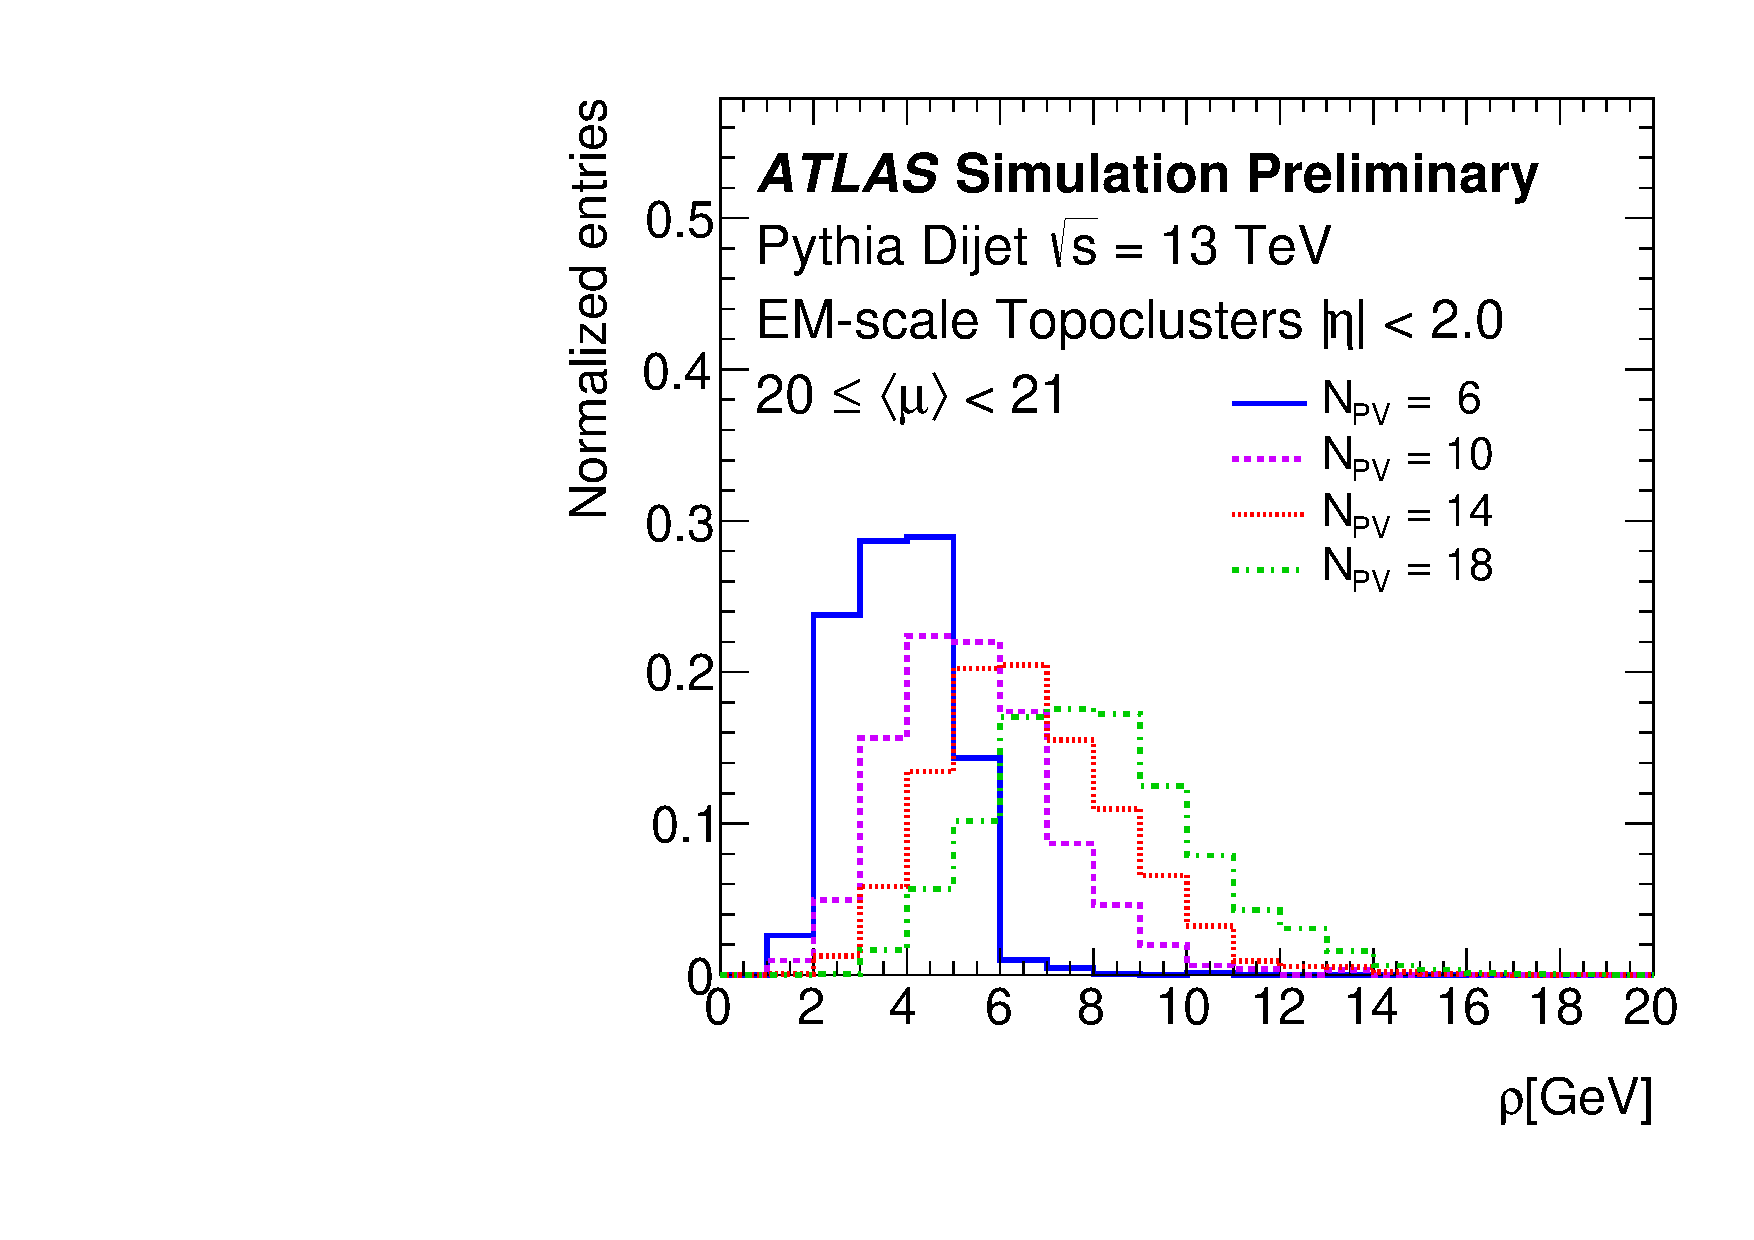
\includegraphics[width=.9\linewidth]{figures/reco/fig_02.pdf}
\caption{ Distribution of event \pt density, $\rho$, taken from \ac{MC} dijets for different numbers of primary vertices. \cite{ATL-PHYS-PUB-2015-015} }
\label{fig:reco_jet_nvtx}
\end{figure}
\end{centering}

\begin{centering}
\begin{figure}[!hbt]
\myfloatalign
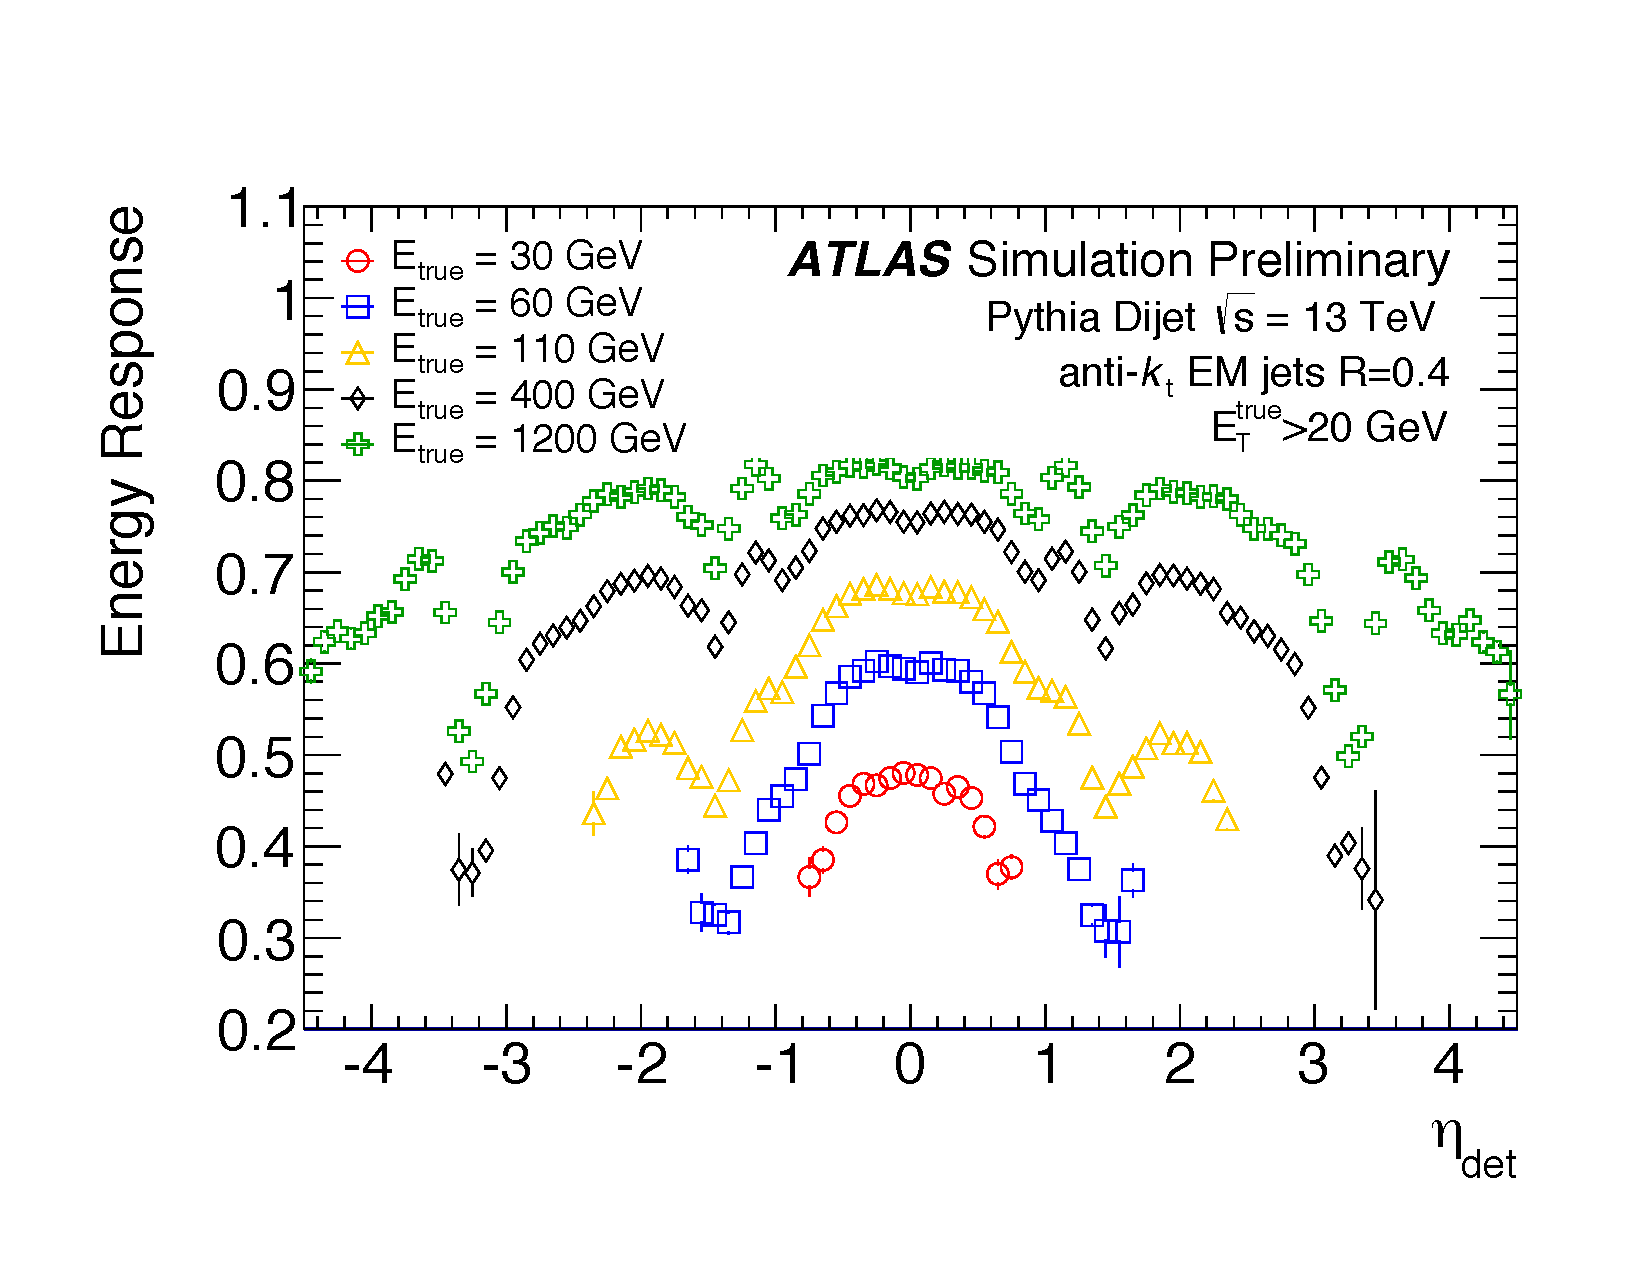
\includegraphics[width=.9\linewidth]{figures/reco/fig_04a.pdf}
\caption{ Energy response as a function of energy and $\eta$ for \ac{EM} jets in dijet \ac{MC}. \cite{ATL-PHYS-PUB-2015-015} }
\label{fig:reco_JES}
\end{figure}
\end{centering}

In addition to correcting for additional energy due to pile-up, it is necessary to reject reconstructed jets that come from pile-up vertices. To accomplish this, a multivariate alogrithm called \ac{JVT} was created which builds upon an older method, \ac{JVF} \cite{ATLAS-CONF-2014-018}. 

\ac{JVF} gives the fraction of energy in a jet that comes from the hard-scatter vertex, and is defined as 

\begin{equation}
\mathrm{JVF} = \frac{\sum_i \pt^i(PV_0)}{\sum_j \pt^j(PV_0) + \sum_{n\geq1} \sum_j \pt^j(PV_n)} 
\end{equation}

where $\pt^i(PV_n)$ gives the \pt of the $i$th track associated with the $n$th primary vertex. $PV_0$ gives the primary vertex associated with the hard-scattering, while the remaining vertices are due to pile-up interactions. Track are associated with a jet according to a processes called \textit{ghost association}, in which they are clustered along with the typical pseudo-jet collection according to the anti-$k_t$ algorithm described above. In the clustering process, the tracks energy is ignored so that it doesn't impact the measurement of the final jet. 

This fraction decreases with higher pile-up, making the construction of an explicit cut difficult in varying pile-up conditions. \ac{JVT} improved on the method by using a pile-up corrected \ac{JVF}-like variable, defined as 

\begin{equation}
\mathrm{corrJVF} = \frac{\sum_i \pt^i(PV_0)}{\sum_j \pt^j(PV_0) + \frac{\sum_{n\geq1} \sum_j \pt^j(PV_n)}{kn_{PU}}} 
\end{equation}

where $n_{PU}$ is the number of tracks, which is multiplied by a scaling factor $i = 0.01$. This quantity is included in the inputs of the tagger along with other variables measuring the fraction of jet energy that is associated with the hard-scattering vertex. \autoref{fig:reco_jvt} shows the efficiency and fake rate for the two methods, demonstrating \ac{JVT}'s superior stability across events with different numbers of pile-up vertices. 

\begin{centering}
\begin{figure}[!hbt]
\myfloatalign
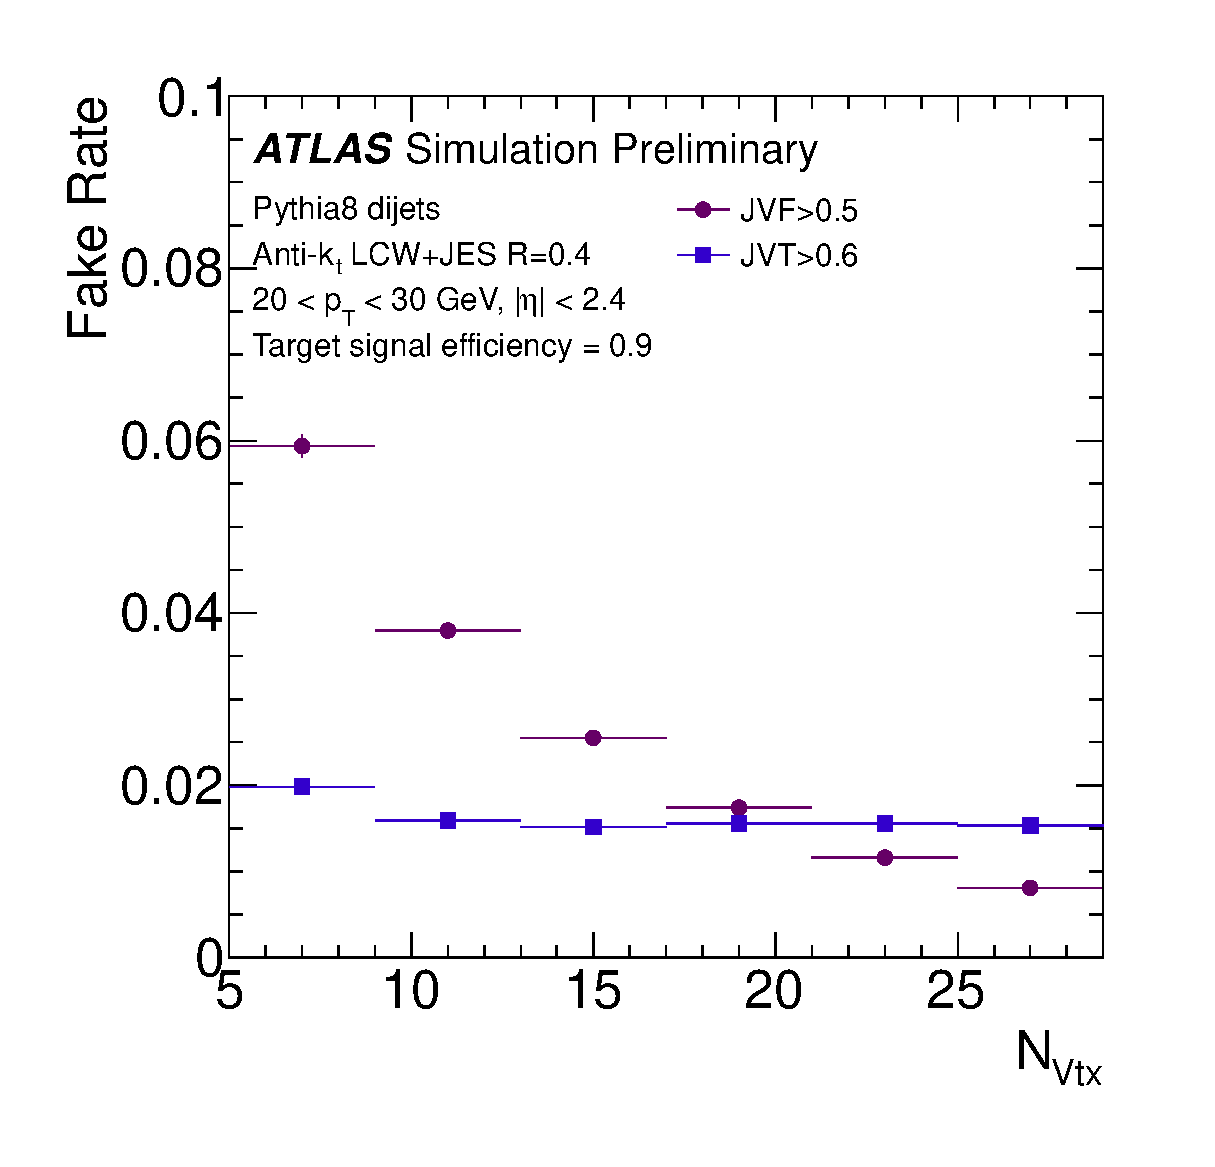
\includegraphics[width=.48\linewidth]{figures/reco/jvt_fig_06b.eps}
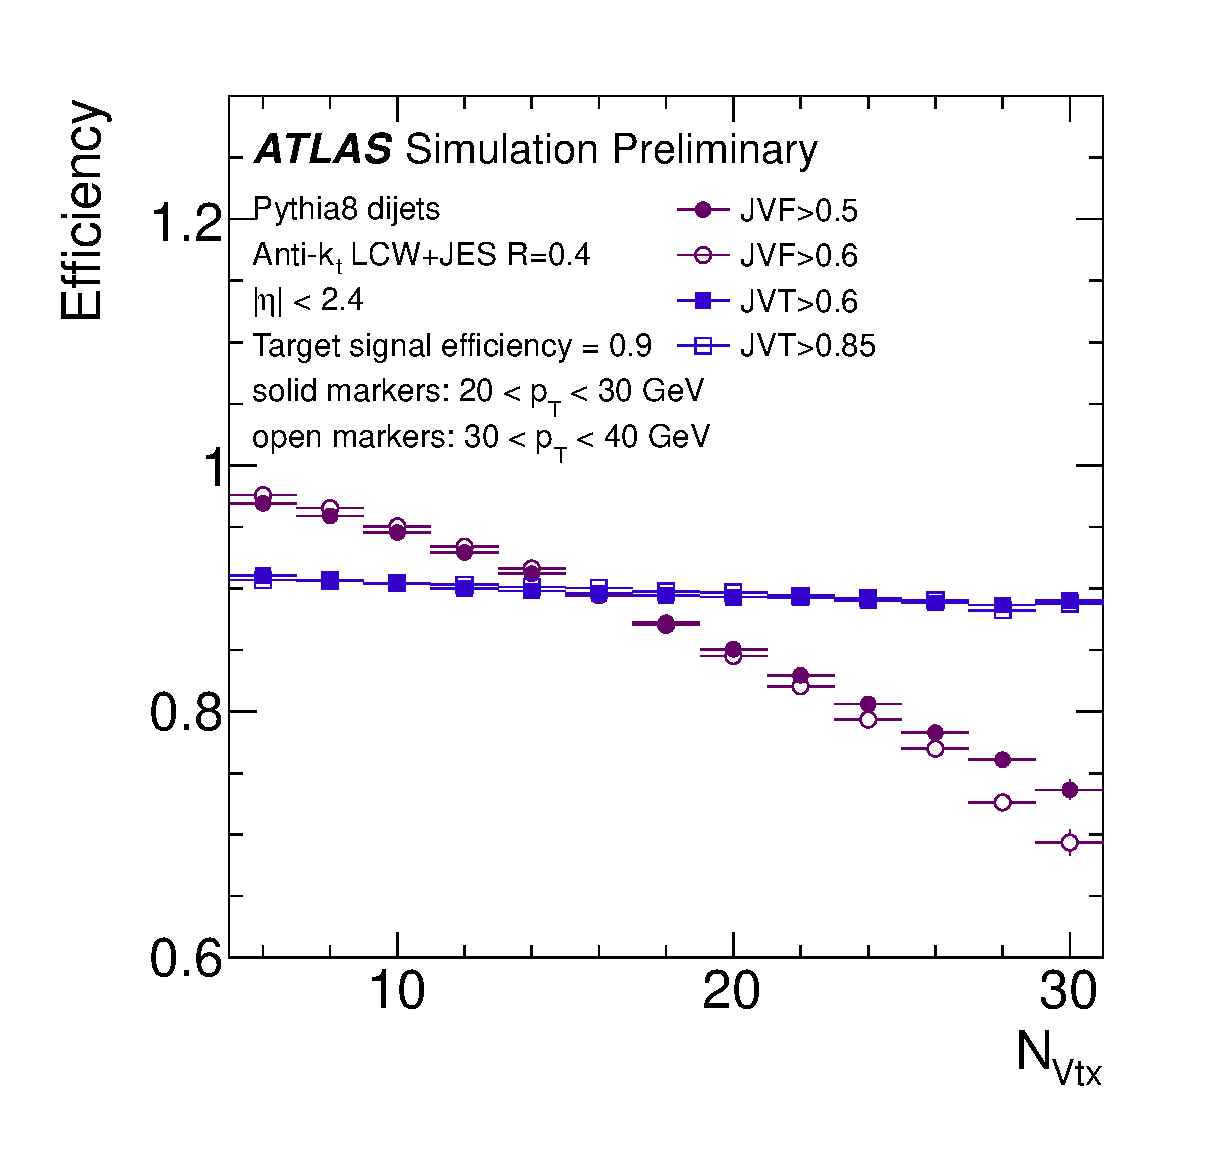
\includegraphics[width=.48\linewidth]{figures/reco/jvt_fig_07a.eps}
\caption{ Dijet \ac{MC} distributions of the number of pile-up jets passing the \ac{JVT} and \ac{JVF} cuts (left) and the efficiency for jets from the primary vertex (right) as a function of number of primary vertices in the event \cite{ATLAS-CONF-2014-018}. }
\label{fig:reco_jvt}
\end{figure}
\end{centering}

It is possible to differentiate jets resulting from $b$-hadron decays from other jets due to the non-negligible lifetimes of the hadrons. Many \ac{BSM} processes preferentially produce $b$ quarks, as do any processes involving top quarks, so this identification can be useful for any analyses seeking to isolate these instances. Multivariate techniques are used to identify secondary vertices using the \ac{ID} \cite{ATL-PHYS-PUB-2015-022}. In \ac{ATLAS}, separate algorithms are used to identify jets with tracks with significantly non-zero impact parameters, tracks that reconstruct a secondary vertex, and tracks that can be identified with a chain of vertices beginning with the primary vertex. This information is fed into a boosted decision tree, a type of multivariate algorithm, called \texttt{MV2c20}, which outputs a discriminant shown in \autoref{fig:reco_mv2}. Using this discriminant, a working point is chosen such that $b$-jets can be identified with a 70\% efficiency, with mis-identification rates at around 12\% for $c$-jets and 0.2\% for light-flavor jets.

\begin{centering}
\begin{figure}[!hbt]
\myfloatalign
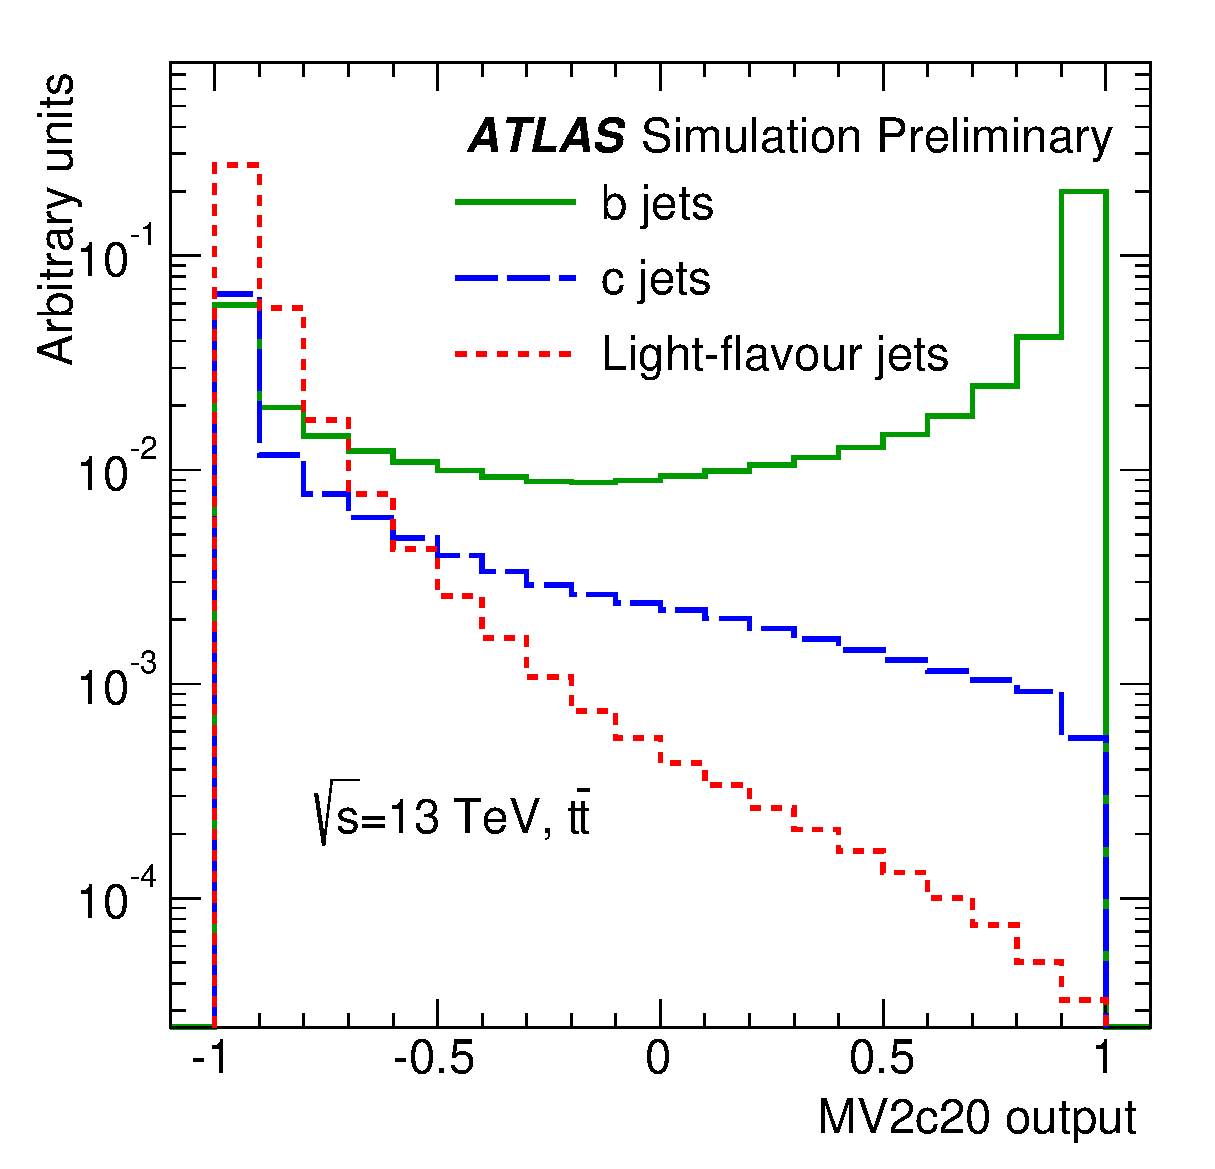
\includegraphics[width=.9\linewidth]{figures/reco/fig_08.eps}
\caption{ Distribution of \texttt{MV2c20} output for $b$-jets, $c$-jets, and light-flavor jets in \ttbar \ac{MC} \cite{ATL-PHYS-PUB-2015-022}. }
\label{fig:reco_mv2}
\end{figure}
\end{centering}

\section{Overlap Removal}
\label{sec:reco_or}

Because most of these reconstruction methods are run independently, it is common for energy deposits and tracks to be shared between jets and particles of different types. To account for this, a process called \acf{OR} is used, which iteratively removes overlapping objects. The process, as well as the calculation of missing transverse momentum described in \autoref{sec:reco_met}, is performed on \textit{baseline} objects. These objects have looser selections than the final \autoref{signal} objects, and the separate definitions allow analyzers to tune signal objects to best match a \ac{BSM} signature, while leaving the \ac{OR} process unchanged. The signal and baseline definitions for this analysis are described in \autoref{ch:objects}.

The first step in the \ac{OR} process is to remove reconstructed jets that appear to be due to calorimetric deposits from an electron. To accomplish this, any baseline jet within $\Delta R = 0.2$ from a baseline electron is removed. A caveat is added due to the frequent production of leptons in the decay of heavy-flavor jets; if the jet is $b$-tagged, the electron will be removed instead. After these electrons and jets have been removed, a new search is done for jets and electrons within $\Delta R = 0.4$ of one another. In this iteration, the electron is removed, again to reduce backgrounds from heavy-flavor decays.

Next, the muon-jet \ac{OR} is applied, which is very similar to that of the electron. Any jet within $\Delta R = 0.2$ of a muon is removed, unless the jet is $b$-tagged, in which case the muon is removed due to the likelihood that it resulted due to a heavy-flavor decay. The muon-jet \ac{OR} then differs from the electron's in that a \pt-based $\Delta R$ cut is used in the last step. Muons within $\Delta R < \mathrm{min}(0.04 + (10 \gev)/\pt, 0.4)$ of a jet are removed, with the \pt-dependent cone size designed to reject low-\pt heavy-flavor muons while preserving muons resulting from the decay of high-\pt particles, which are closely aligned with the other products of the decay. 

The next step is to remove electrons resulting from muon bremsstrahlung. Any electron within $\Delta R = 0.1$ of a muon is removed from the event. 

Lastly, overlap between photons and both jets and electrons is considered. Baseline photons within $\Delta R = 0.4$ of an electron are removed, as are jets within $\Delta R = 0.4$ of a remaining photon.

\section{Missing Transverse Momentum}
\label{sec:reco_met}

Missing transverse momentum (${\boldsymbol p}_{\mathrm{T}}^\mathrm{miss}$, with magnitude \met), is the negative vector sum of \pt measured in an event. Because the colliding protons have no initial transverse momentum, the true value of this quantity should be zero unless a particle escapes the detector without being measured, as neutrinos do. In practice, the reconstructed \met can also be non-zero due to mismeasurement, or due to gaps in the \ac{ATLAS} detector. \met reconstruction is perhaps the most complex because it depends on all other object reconstructions performed in the \ac{ATLAS} detector. 

\met components are calculated independently for each type of baseline object reconstructed, as well as for a soft term, which comprises the energy observed by the \ac{ATLAS} detector but not associated with a baseline object. The soft term can be calculated based either on calorimeter or track measurements \cite{ATL-PHYS-PUB-2015-023}. While the \acf{CST} is very sensitive to pile-up, the \acf{TST} is much more robust, as it excludes tracks emanating from pile-up vertices. Tracks associated with any reconstructed object are also removed. \autoref{fig:reco_met_tst} shows the dependence of the \ac{TST} resolution on number of primary vertices. Because of this lessened pile-up dependence, the \ac{TST} is used to reconstruct \met in this analysis. 

\begin{centering}
\begin{figure}[!hbt]
\myfloatalign
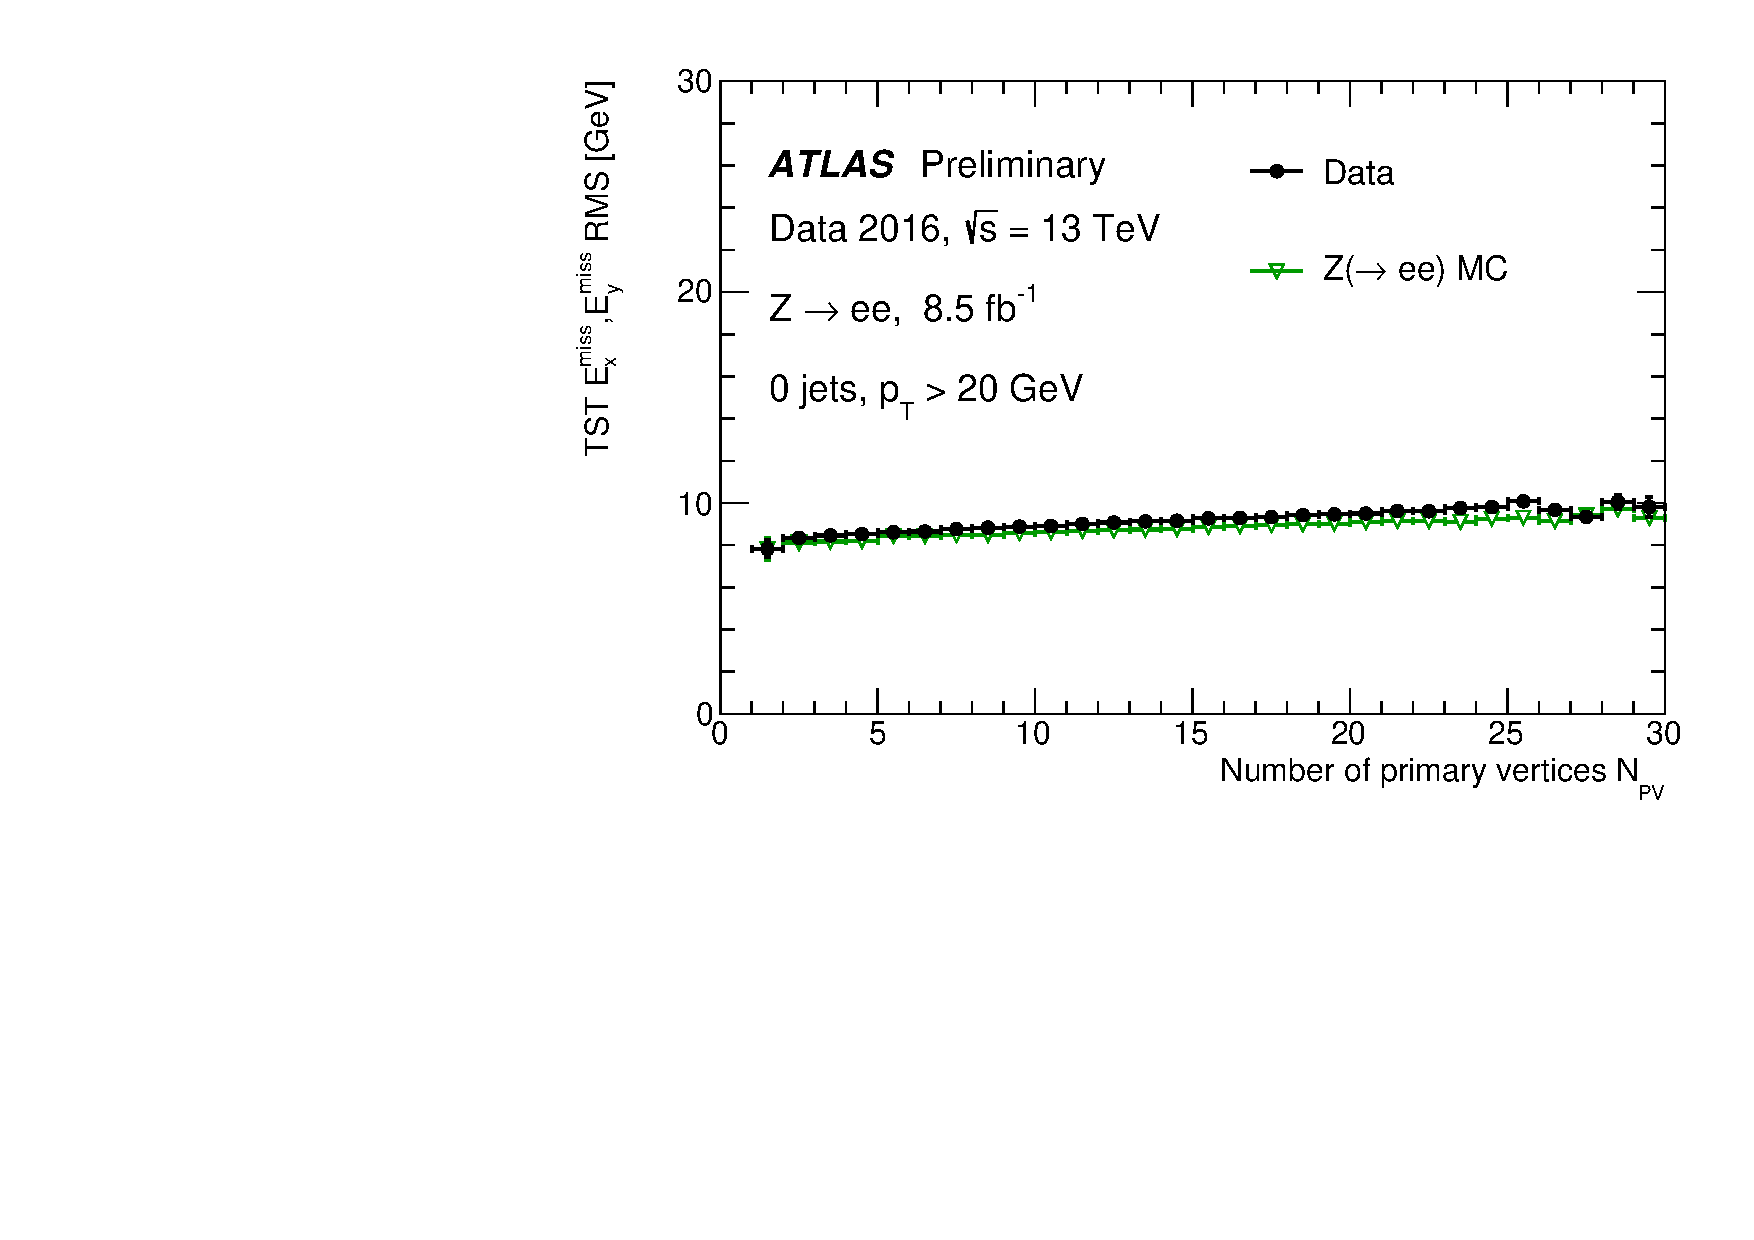
\includegraphics[width=.9\linewidth]{figures/reco/mettst.pdf}
\caption{ Distributions of the resolution of the $x$ and $y$ components of \ac{TST} \met in $Z\rightarrow\mu\mu$ events in data and \ac{MC}. }
\label{fig:reco_met_tst}
\end{figure}
\end{centering}

$Z\rightarrow\mu\mu$ events, which rarely have any true \met, can be used to study the contribution of different objects to the total \met calculation. \autoref{fig:reco_met_terms} shows the the \met resulting from muons, jets, and the soft term measured in events with two opposite-sign muons that reconstruct an invariant mass within 25 \gev~of the $Z$ boson mass. Because very little real \met exists, these distributions primarily demonstrate how mismeasurement of various objects contributes to the \met term. Though the soft term falls off very quickly, rarely producing events with more than 50 \gev~of \met, both the jet and muon distributions have longer tails, producing more events with higher \met. 

\begin{centering}
\begin{figure}[!hbt]
\myfloatalign
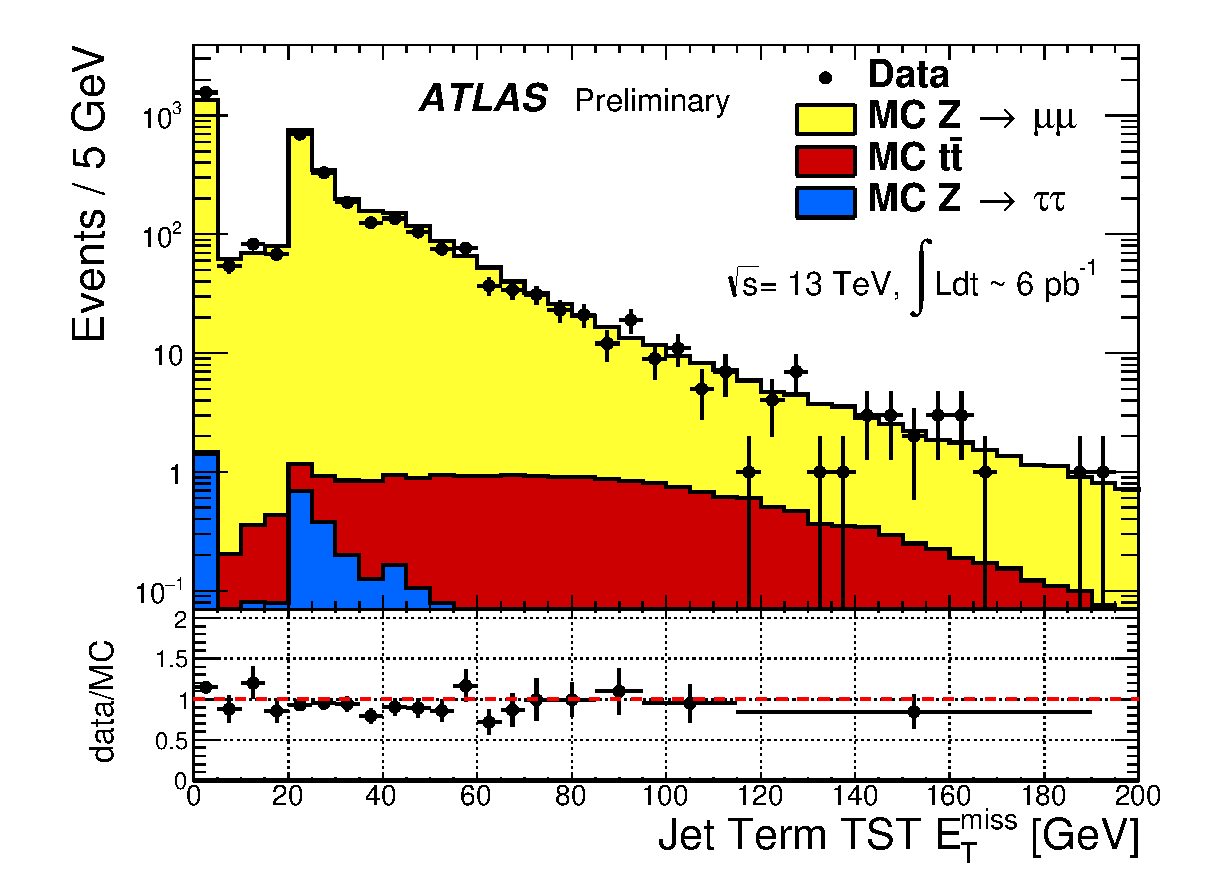
\includegraphics[width=.48\linewidth]{figures/reco/met_fig_02a.eps}
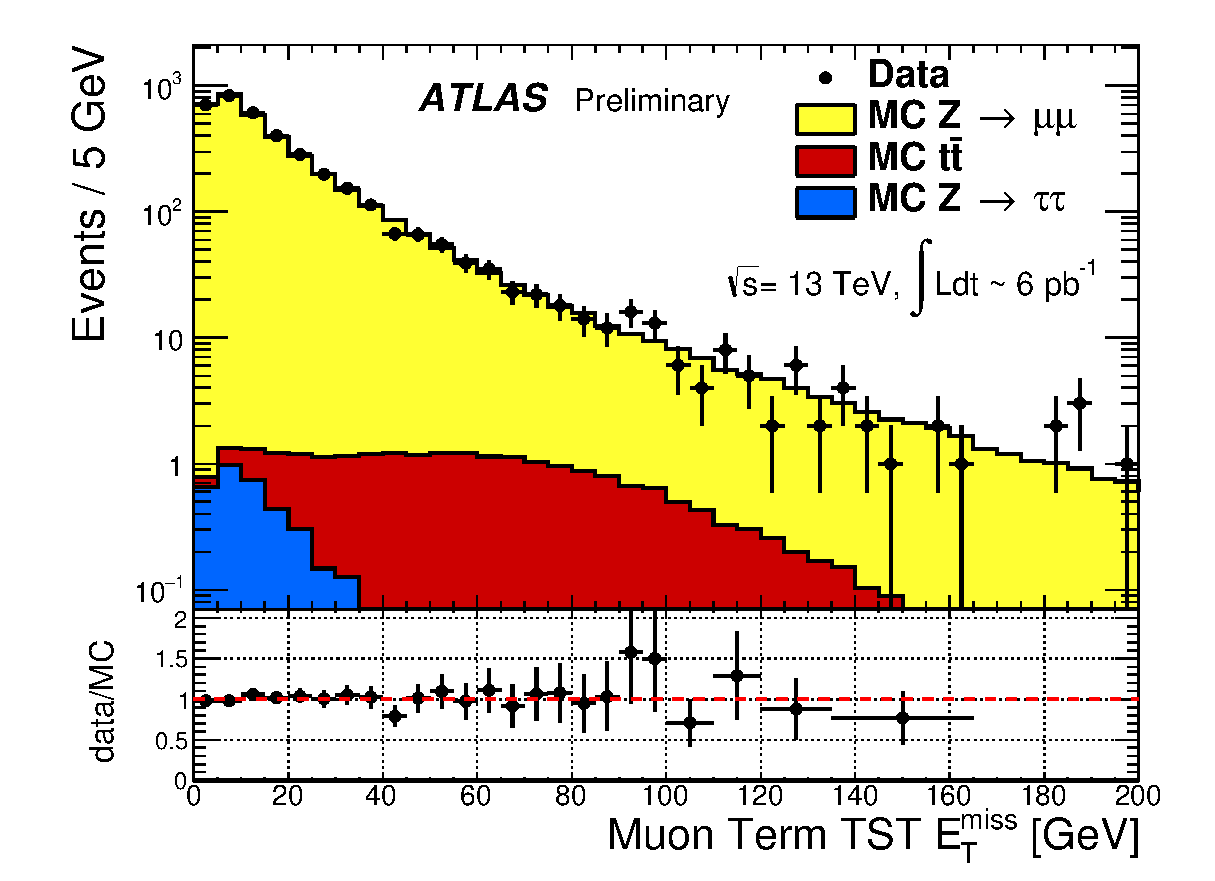
\includegraphics[width=.48\linewidth]{figures/reco/met_fig_02b.eps} \\
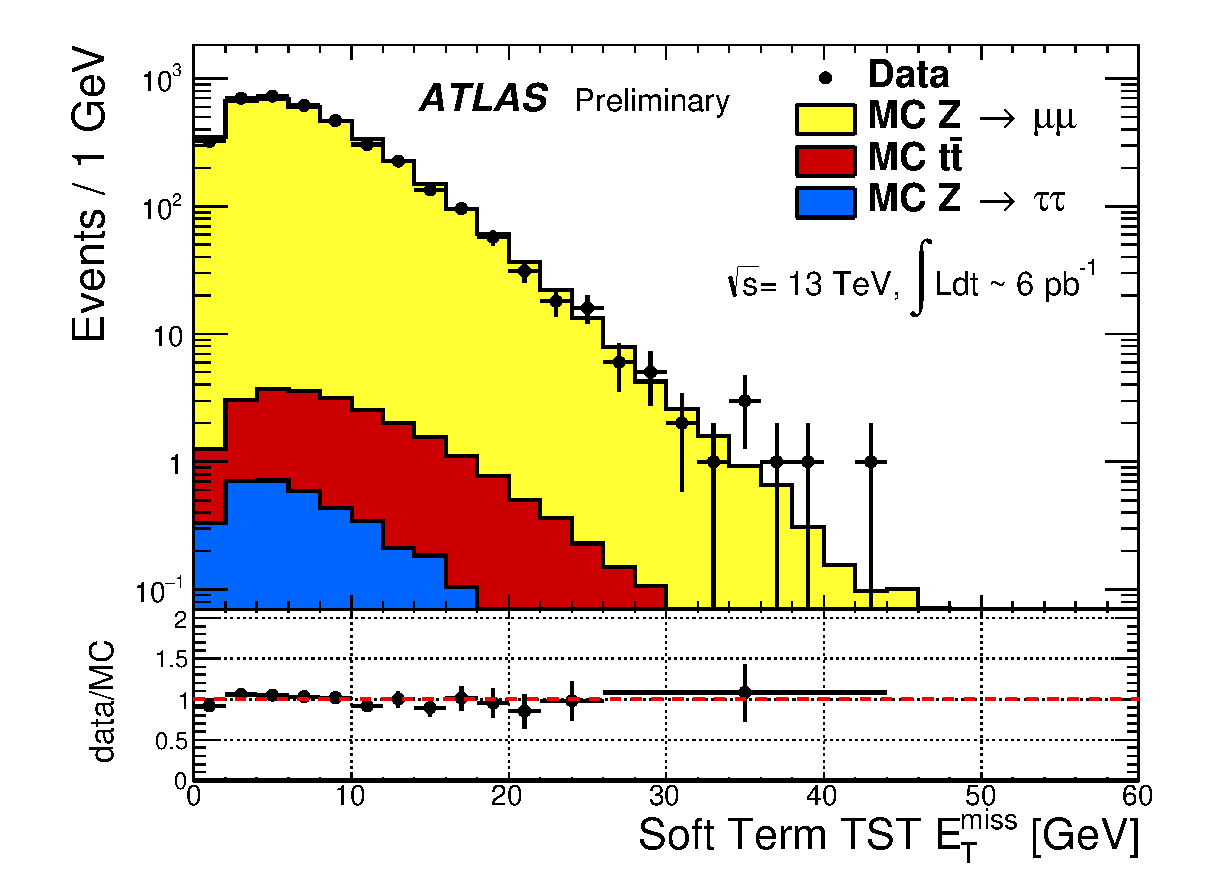
\includegraphics[width=.48\linewidth]{figures/reco/met_fig_02c.eps}
\caption{ Distributions of the jet term (top left), muon term (top right), and \ac{TST} (bottom) \met in $Z\rightarrow\mu\mu$ events in data and \ac{MC}. In the jet term distribution, the feature at zero is due to events with no jets, and the spike at 20 \gev~corresponds to the minimum jet \pt considered for the analysis \cite{ATL-PHYS-PUB-2015-027}. }
\label{fig:reco_met_terms}
\end{figure}
\end{centering}




 % Reconstruction
% Chapter 3

\chapter{Application of a Neural Network to Pixel Clustering} % Chapter title

\label{ch:nn} % For referencing the chapter elsewhere, use \autoref{ch:mathtest}

%----------------------------------------------------------------------------------------

%----------------------------------------------------------------------------------------

\section{Clustering in the Pixel Detector}

Creating tracks from individual hits in the Inner Detector is one of most computationally challenging parts of the reconstruction of ATLAS events. Each event typically contains thousands of hits in the pixel detector alone, which must be combined into one coherent picture of which particles traversed the detector, and how they moved and lost energy as they traveled. A typical particle deposits charge in several pixels per layer, forming a series of clusters which can be connected together to form a track. This track can in turn be used to measure the charge, momentum, and trajectory of the particle, and in many cases, provides ATLAS's most precise measurement of a charged particle. 


\begin{centering}
\begin{figure}[bth]
\myfloatalign
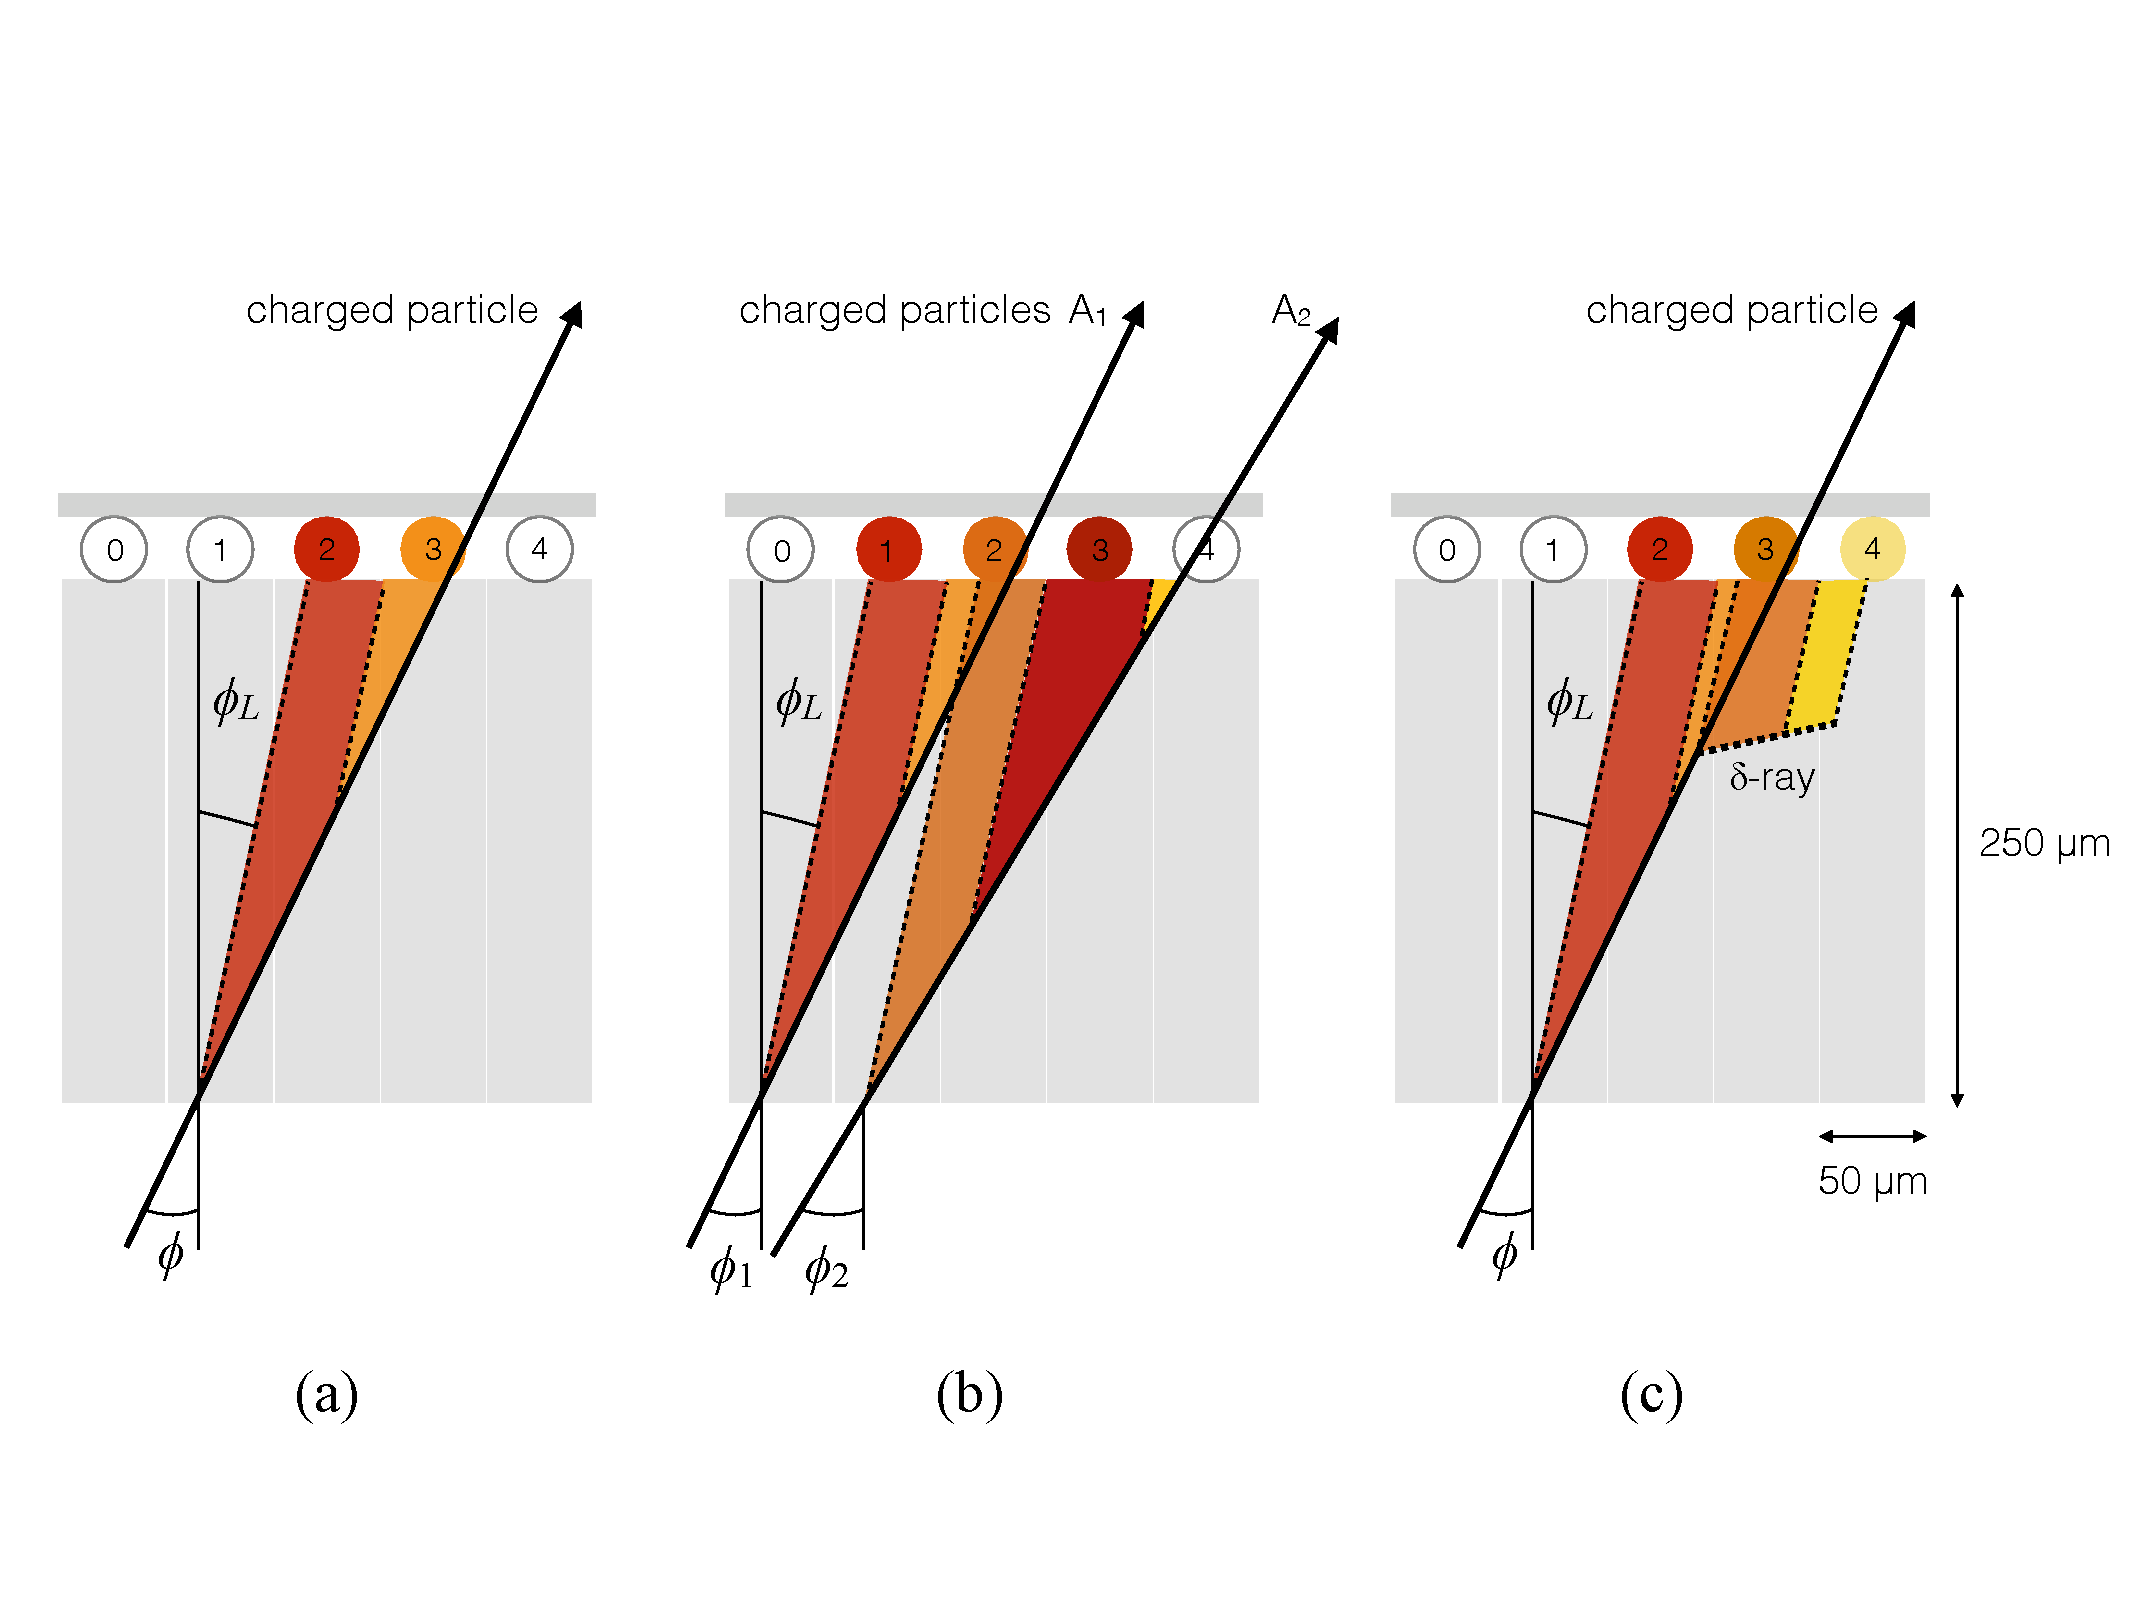
\includegraphics[width=.90\linewidth]{figures/nn/cluster_types.pdf}
\caption{A few possible types of clusters in the Pixel Detector. $(a)$ shows a single particle passing through a layer of the detector, $(b)$ shows two particles passing through the detector, creating a single merged cluster, and $(b)$ shows a single particle emitting a $\delta$-ray as it passes through the detector.}
\label{fig:cluster_types}
\end{figure}
\end{centering}

The process of going from clusters to track is relatively simple in an isolated environment in which one particle travels cleanly through all the layers, but can be complicated by multiple close-by tracks and by a single particle's emission of low energy particles, called $\delta$-rays. In these cases, it can be hard to tell how many particles were involved in creating a cluster, and where exactly each of those particles passed through the layer. A few examples of these cases can be seen in \autoref{fig:cluster_types} . The process of determining this is called Clustering, and it has recently been updated from a charge interpolation method to a method using a \ac{NN}. 

\subsection{Charge Interpolation Method}

A typical cluster contains a few pixel hits spanning in the $x$ and $y$ directions, each with its own measurement of charge deposition, or \ac{ToT}. The extent of the cluster is defined by grouping together any pixels with a shared edge or corner. In the charge interpolation method, also called the \ac{CCA} clustering algorithm, these individual hits are combined to make one estimation of the position a single particle which passed through them, using the following equation: 

\begin{eqnarray}
x_{cluster} = x_{center} + \Delta_x(\phi,N_{row}) \cdot \left[ \Omega_x -\frac{1}{2} \right] \\
\label{eq:analogx}
x_{cluster} = x_{center} + \Delta_x(\phi,N_{row}) \cdot \left[ \Omega_x -\frac{1}{2} \right]
\label{eq:analogy}
\end{eqnarray}

where $\Omega_{x(y)}$ is defined by

\begin{equation}
\Omega_{x(y)} = \frac{q_{last~row(col)}}{q_{first~row(col)} + q_{last~row(col)}}
\end{equation}

and $q$ represents the \ac{ToT} of a given pixel, and $\Delta_{x(y)}$ is a function derived from either data or \ac{MC} and produces an output related to the projected length of the particles track on the pixel sensor and is measured as a function of $\phi$, the incident angle of a particle on the sensor, and $N_{row(col)}$, the number of pixels in the $x$ and $y$ direction. 

In a simple case, such as $(a)$ of \autoref{fig:cluster_types} , this method works quite effectively. However, in cases like $(b)$, it has no ability distinguish two-particle from one-particle clusters, and can only assign a cluster center between the two particles' locations, despite that intermediate pixel having the lowest \ac{ToT}. Furthermore, because this method can't differentiate two-particle clusters, the tracking software can't use that information to preferentially allow multiple tracks to be fit to the cluster. In cases like $(c)$, the $\delta$-ray will bias the measurement of the particle's position in whichever direction it is emitted. 

\subsection{Improving Measurement with Neural Networks}

To address these problems, a series of \acp{NN} were created \cite{PERF-2012-05}. The first determines the number of particles in a given cluster, the second predicts their positions with the cluster, and the third assesses the resolution of the position measurement. 

These \acp{NN} are all trained with: 
\begin{itemize}
\item a $7\times7$ grid of cluster \ac{ToT} information\footnote{Clusters spanning more than seven pixels in either direction are split into multiple clusters.}
\item a seven-element vector containing the $y$-size of the pixels in the grid
\item the layer number of the cluster
\item a variable indicating whether the cluster located in the barrel or endcap
\item $\theta$ and $\phi$ variables projecting the incident angles of the particle on the sensor, assuming it comes from the interaction point
\item the $\eta$ index of the pixel module
\end{itemize}

After the Number \ac{NN} predicts a number of particles associated with the cluster, required to be between 1 and 3, the same inputs are fed to one of three Position \acp{NN} based on the determined number of particles, which then outputs the $x$ and $y$ positions of each of the particles. Then, the same inputs combined with the output of the Position \ac{NN} are fed into one of three Error \acp{NN} (also distinguished by number of particles), which outputs a resolution for each of the position predictions made. An example of the output of this process can be seen in \autoref{fig:merged_cluster}, where the improved position resolution from the ability to identify a multi-particle cluster is evident. The particle location predictions from the \acp{NN} are then handed to the tracking software, which is able to independently consider multiple locations from a given cluster to find the best fit. 

\begin{centering}
\begin{figure}[bth]
\myfloatalign
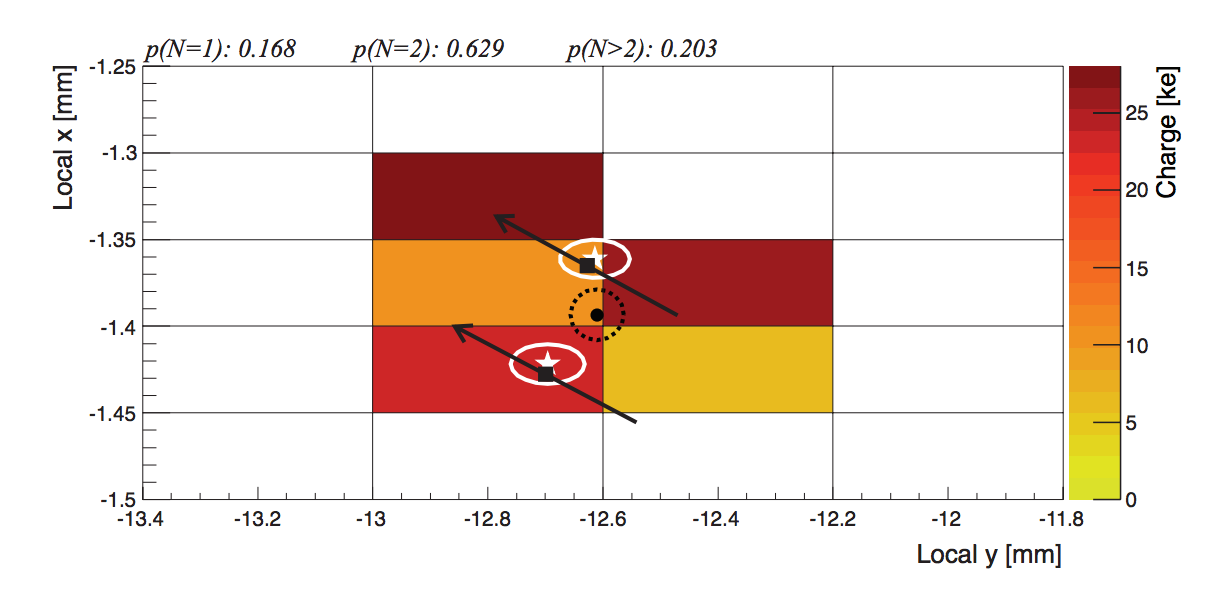
\includegraphics[width=.90\linewidth]{figures/nn/merged_cluster.png}
\caption{One example of a two-particle cluster and its truth information compared with the output of the \acp{NN}. At top, the $p(N=i)$ values give the output of the Number \ac{NN}, the probabilities that the cluster contains 1, 2, and 3 particles. Given the highest probability is for $N=2$, the other \acp{NN} predict the postion and errors of the two particles (in white). The black arrows and squares represent the truth information from the cluster, and the black dot and dotted line show the position measurement for the un-split cluster.}
\label{fig:merged_cluster}
\end{figure}
\end{centering}

\section{Impact of the Neural Network}

The \ac{NN} was first applied to $7 TeV$ data, where it improved position resolution for particles in small and large clusters. \autoref{fig:7tev_res} shows the improvement from the addition of the \ac{NN} in $x$ resolution in different cluster sizes. The improvement from \ac{CCA} clustering is particularly evident in the 4-pixel case, where the double peaked structure of the interpolation method has been completely removed with the \ac{NN}.  

\begin{centering}
\begin{figure}[bth]
\myfloatalign
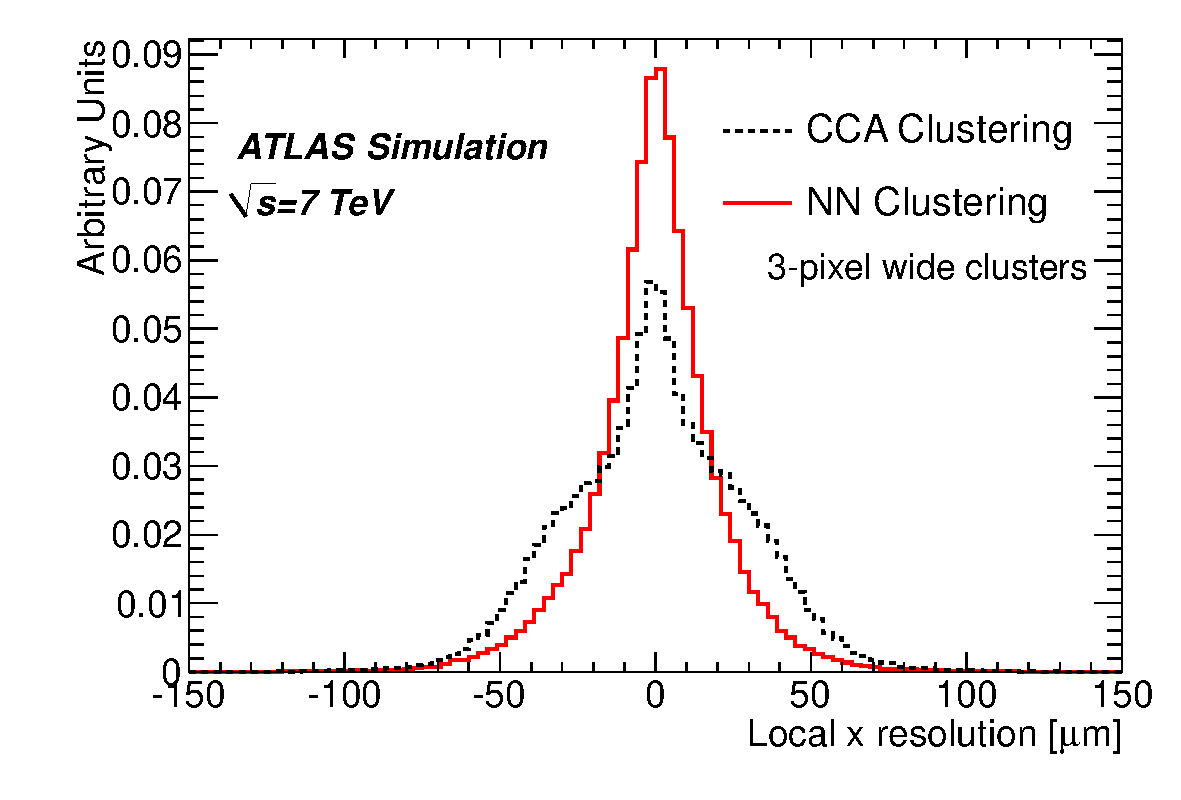
\includegraphics[width=.45\linewidth]{figures/nn/3x_res.pdf}
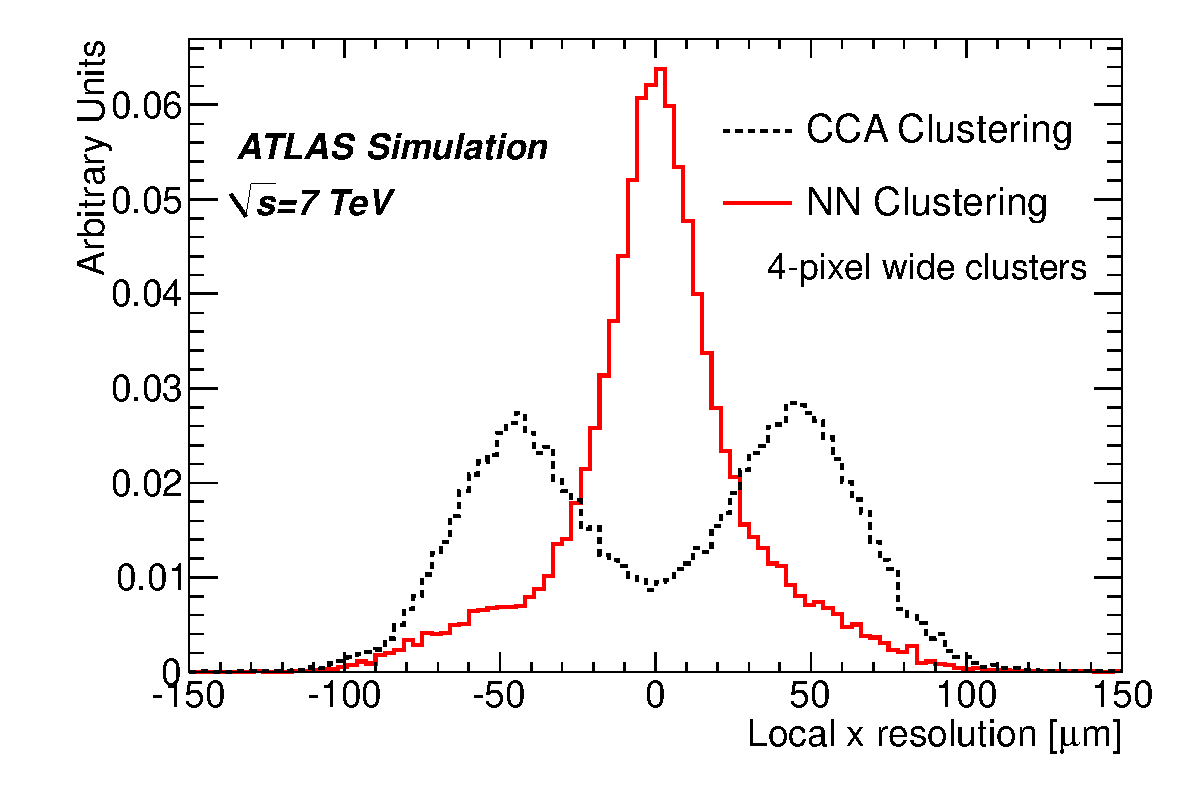
\includegraphics[width=.45\linewidth]{figures/nn/4x_res.pdf}
\caption{$x$ resolutions for clusters with 3 (left) and 4 (right) pixels in the $x$ direction in $7 TeV$ data for \ac{CCA} and \ac{NN} clustering.}
\label{fig:7tev_res}
\end{figure}
\end{centering}

\subsection{The Neural Network in 13 TeV Data}

In Run 2, tracking algorithm is first run on the \ac{CCA} clusters, where it constructs loose tracks that allow shared clusters, clusters to which multiple tracks are fit. The \ac{NN} is then used to identify which clusters are likely to have had multiple particles pass through them, and to identify the positions of those particles. In the case that the cluster is determined to have resulted only from one particle, tracks that share that cluster are penalized. 

Performance in 13 TeV \cite{ATL-PHYS-PUB-2015-044}. 

Robustness \cite{ATL-PHYS-PUB-2015-052}
 % NN

\cleardoublepage % Empty page before the start of the next part

%------------------------------------------------

\ctparttext{This section describes an analysis of the ATLAS data carried out by the author and her analysis team. The analysis was performed on events from $p-p$ collisions provided by the \ac{LHC} at $\sqrt{s}$=13 TeV. It searches for events like those described in \autoref{sec:simplified_models}, which contain a Z boson decaying to leptons, jets, and missing transverse energy. The selection of a signal region in which to search for these events, background estimates, systematic uncertainty estimates, results, and interpretations are all discussed.} % Text on the Part 2 page describing the content in Part 2

\part{Searching for Supersymmetry} % Second part of the thesis
\label{part:search}

% Chapter 7

\chapter{Background Processes} % Chapter title

\label{ch:background_processes} 

%----------------------------------------------------------------------------------------

This analysis is fundamentally a search for \ac{SUSY} in events with two leptons whose invariant mass (\mll) is consistent with a $Z$ boson. Additional event selections are made to reduce \ac{SM} processes relative to potential \ac{SUSY} processes, defined by simplified models discussed in \autoref{sec:simplified_models}. These models include the production of strongly-charged, high-mass particles, which results in events with jets and high \HT, the scalar sum of the \pt of all jets and the two leading leptons in the event. These $R$-parity conserving \ac{SUSY} models also produce decay chains that terminate with a stable, electrically neutral particle, which produces \MET when it passes through \ac{ATLAS} without detection. Each of these features can help isolate these signal events from \ac{SM} backgrounds. To understand what cuts would optimize the sensitivity of the search, it is essential to first understand what these \ac{SM} backgrounds are. 

\begin{centering}
\begin{figure}[bth]
\myfloatalign
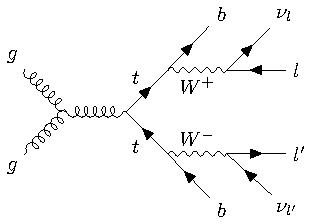
\includegraphics[width=.70\linewidth]{feynman/ttbar.pdf}
\caption{An example Feynman diagram of \ttbar production and decay.}
\label{fig:ttbar}
\end{figure}
\end{centering}

\paragraph{Top-antitop (\ttbar)} production is the largest background for this search because it often precisely mimics the signature expected from the signal process. \autoref{fig:ttbar} shows a Feynman diagram of this process, which results in two jets, leptons, and neutrinos, which are seen in the detector as \MET. Thus, \ttbar events naturally have high \MET and \HT, jets, and leptons from two different $W$ boson decays, which may coincidentally form an invariant mass consistent with a $Z$ boson. Separating these events from signal processes is very difficult, but some steps can be taken to reduce their impact. The leptons resulting from \ttbar don't originate from the same parent particle, so their invariant mass distribution is very broad compared to processes involving leptons from $Z$ bosons. As a consequence, reducing the width of the \mll~window used to identify $Z$-boson candidates can help to reduce this background. Additionally, for sparticles with a higher mass than that of the top quark, the \HT distribution will typically be larger for signal models than for \ttbar. Though the two \HT distributions overlap significantly for most signal models, a high cut on \HT can help to reduce the \ttbar background relative to a potential signal.  

\begin{centering}
\begin{figure}[bth]
\myfloatalign
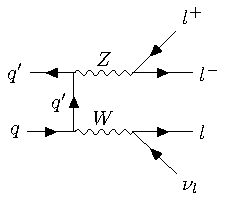
\includegraphics[width=.70\linewidth]{feynman/diboson.pdf}
\caption{An example Feynman diagram of the production and decay of a WZ event.}
\label{fig:diboson}
\end{figure}
\end{centering}

\paragraph{diboson ($VV$)} production is the next leading background. These processes have lower cross-sections than that of \ttbar, but they can also produce events with topologies very similar to signals. Diboson events can contain real $Z$ bosons and their dilepton invariant mass will peak on-$Z$ like a signal. In addition, in events like \autoref{fig:diboson}, an additional $W$ boson can decay to another lepton and a neutrino, producing \MET. The pictured process can occur with associated jets due to initial state radiation, but each additional jet reduces the process's rate by a factor of $\alpha_s$. If the $W$ boson in this figure instead decayed to two jets, which occurs about twice as often as the pictured decay, there would be no true \MET from a neutrino. Thus, introducing a requirement that the signal region include both high amounts of \MET and at least two jets can very effectively reduce the contribution from both these scenarios. A veto on a third lepton could also be used to reduce the contribution from events with $W\rightarrow \ell \nu$ decays, but, depending on the signal model considered, this veto can also decrease signal acceptance. Since the branching ratio for this process is relatively small, the potential reduction in signal acceptance is deemed more important, and a third lepton veto is not used in this analysis. 

\begin{centering}
\begin{figure}[bth]
\myfloatalign
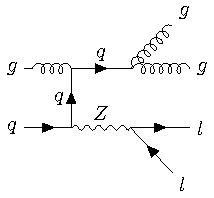
\includegraphics[width=.70\linewidth]{feynman/zjets.pdf}
\caption{An example Feynman diagram of the production and decay of a \dyjets event.}
\label{fig:zjets}
\end{figure}
\end{centering}

\paragraph{\dyjets} processes are very common but, as shown in \autoref{fig:zjets}, don't typically produce any true \MET. The exception is events $Z\rightarrow\tau\tau$ events, which contain \MET because the $\tau$ leptons decay within the detector, and these decays include $\tau$ neutrinos. However, only about 1/3 of $\tau$ decays produce an electron or muon, and even if two leptons are created in an event, they will typically not reconstruct a $Z$ mass due to the energy lost to the neutrinos. For the purposes of this analysis, \textit{lepton} refers only to electrons and muons, and excludes these more complicated $\tau$ events. A high \HT cut helps reduce the \dyjets background, but this process can occur with initial state radiation, producing events with large amounts of hadronic activity. \MET is the most powerful variable for reducing $Z\rightarrow\mu\mu$ and $Z\rightarrow ee$ events, because though events with mismeasured jets or leptons can fake \MET, mismeasurements drastic enough to produce hundreds of \gev~of \met are rare. In addition, events with substantially mismeasured leptons often have \mll~values that are inconsistent with a $Z$ boson, and so a fraction of \dyjets events that do pass a \MET threshold can be excluded nonetheless. 

Other processes can contribute to the \ac{SM} background at lower rates. Processes similar to \dyjets but with a $W$ boson instead of a $Z$ have real \MET from leptonic $W$ decays, but only one lepton. However, a fake or non-prompt lepton can cause these events to look very similar to simulated signals. Single top production can occur in association with a $W$ boson, which produces signatures similar to \ttbar, but with fewer jets.  Additionally, there are \textit{rare top} processes such as \ttbar production in association with $W$ or $Z$ bosons, which are event more difficult to separate from signal events than \ttbar due to the presence of a genuine $Z$ boson, the increased \met from $W$ decays, and the larger amounts of hadronic activity.

Several of these backgrounds are grouped together and referred to as \textit{\aclu{FS}} (\acs{FS}) processes. These include any processes that produce pairs of leptons with uncorrelated flavor in the final state. In this analysis, the largest \ac{FS} background is \ttbar, with additional contributions from $WW$, $Wt$, and $Z\rightarrow\tau\tau$ events. In these processes, each lepton comes from the decay of a different particle. In the case of \ttbar, the two top quarks decay to $W$ bosons, which each produce a lepton in their decays, as shown in \autoref{fig:ttbar}. Consequently, these leptons' flavors are correlated with the flavor of the neutrino that results from the same boson's decay, but not with one another.

\section{Data and Monte Carlo Samples} 

This analysis uses data collected by the \ac{ATLAS} detector from $pp$ collisions at a center-of-mass energy of 13 \tev~in 2015 and 2016, corresponding to a total luminosity of 14.7 fb$^{-1}$. The data collected use a combination of unprescaled single and dilepton triggers, discussed in greater detail in \autoref{sec:trig_strategy}. The triggers targeting the lowest \pt ranges are fully efficient for pairs of leptons with \pt of at least 20 \gev. In addition, photon events are collected for use in a control region using both prescaled and unprescaled triggers, with the lowest trigger threshold at 35 \gev~in 2015 and 20 \gev~in 2016. 

\ac{MC} samples are generated for each background process that appears in the signal and validation regions. \autoref{tab:MC} details the generators used to produce each sample, and more information can be found in \autoref{sec:MC_gen}. These simulated background events, in conjunction with the simulated signal discussed in \autoref{sec:simplified_models}, are used to determine approximate sensitivities of the search and optimize signal regions. The background \ac{MC} also provides a valuable cross-check for many of the data-driven background estimates discussed in \autoref{ch:backgrounds}, and in the case of rare top and some diboson events, provides the primary estimate of the background.

\begin{sidewaystable*}[ht]
\begin{center}
\caption{Simulated background event samples used in this analysis with the corresponding matrix element and parton shower generators,
cross-section order in $\alpha_{\text{s}}$ used to normalize the event yield, underlying-event tune and PDF set.
}
\scriptsize
\begin{tabular}{l c c c c c }
\hline
Physics process &  Generator  & Parton & Cross section & Tune & PDF set\\
                &             & Shower &              &      & \\
%\hline\hline
\noalign{\smallskip}\hline\noalign{\smallskip}
$t\bar{t}+W$ and $t\bar{t}+Z$~\cite{ATL-PHYS-PUB-2016-005,Garzelli:2012bn}& {\sc MG5\_aMC@NLO}        & {\sc Pythia} 8.186 & NLO \cite{Campbell:2012,Lazopoulos:2008} & {\sc A14} & NNPDF23LO\\
$t\bar{t}+WW$~\cite{ATL-PHYS-PUB-2016-005}      & {\sc MG5\_aMC@NLO}          & {\sc Pythia} 8.186 & LO \cite{Alwall:2014hca} & {\sc A14}  &  NNPDF23LO\\
$t\bar{t}$~\cite{ATL-PHYS-PUB-2016-004}         & {\sc Powheg Box v2} r3026   & {\sc Pythia} 6.428 & NNLO+NNLL \cite{ttbarxsec1,ttbarxsec2}          &\sc{Perugia2012}     &NLO CT10\\
Single-top ($Wt$)~\cite{ATL-PHYS-PUB-2016-004}  & {\sc Powheg Box v2} r2856   & {\sc Pythia} 6.428 & Approx. NNLO \cite{Kidonakis:2010b}& \sc{Perugia2012}    &NLO CT10 \\ 
$WW$, $WZ$ and $ZZ$~\cite{ATL-PHYS-PUB-2016-002} & \sherpa\ 2.1.1 & \sherpa\ 2.1.1 & NLO \cite{diboson1,diboson2} & \sherpa\ default & NLO CT10 \\
%$WZ$ and $ZZ$~\cite{ATL-PHYS-PUB-2016-002} &&& \\ 
$Z/\gamma^{*}(\rightarrow \ell \ell)$ + jets~\cite{ATL-PHYS-PUB-2016-003}& \sherpa\ 2.1.1           & \sherpa\ 2.1.1  &NNLO \cite{DYNNLO1,DYNNLO2}       & \sherpa\ default     &NLO CT10\\
\gjets & \sherpa\ 2.1.1 & \sherpa\ 2.1.1 & LO~\cite{sherpa} & \sherpa\ default & NLO CT10 \\
$V(=W,Z)\gamma$ & \sherpa\ 2.1.1 & \sherpa\ 2.1.1 & LO~\cite{sherpa} & \sherpa\ default & NLO CT10 \\
signal & {\sc MG5\_aMC@NLO} & {\sc Pythia} 8.186 & NLO & A14 & NNPDF23LO\\
\noalign{\smallskip}\hline\noalign{\smallskip}
\end{tabular}
\label{tab:MC}
\end{center}
\end{sidewaystable*}
 % Background Processes 
% Chapter 8

\chapter{Object Identification and Selection} % Chapter title
\label{ch:objects} 

This section describes the identification and selection of objects in the events of this analysis. Objects have \textit{baseline} definitions, which are used for \acf{OR} and the calculation of \met, then have tighter \textit{signal} definitions, which defines the objects considered in the final analysis of the kinematics of events. Definitions are presented for electrons, muons, and jets, which are all required in the \ac{SR} of the analysis, as well as photons, which are used in background estimation. This section refers to quality definitions described in \autoref{ch:reconstruction}.

%----------------------------------------------------------------------------------------

\section{Electrons}

Electrons are reconstructed using the Egamma algorithm discussed in \autoref{sec:reco_electrons}. All electrons are required to be within $|\eta|<2.47$, to ensure that all tracks are consistently within the tracking capability of the \ac{ID}. Baseline leptons are required to have $\pt>10\gev$ and pass the \texttt{LHLoose} quality standard. Signal leptons are further required to be of \texttt{LHMedium} quality with \texttt{GradientLoose} isolation, and must have $\pt>25\gev$. Additional cuts on impact parameter are made for electrons with the goal of identifying only electrons coming from the primary vertex of the event, the vertex with the highest associated \pt. These requirements, and all the other requirements made on the electrons can be seen in \autoref{tab:eledef}. 

\begin{table}[ph!]
\begin{center}
    \begin{tabular}{l|c}
      \hline
      Cut            & Value/description \\
      \hline
      \hline
      \multicolumn{2}{c}{Baseline Electron}\\
      \hline
      Acceptance   & $\pt > 10\,\GeV, |\eta^\mathrm{clust}| < 2.47$ \\
      Quality      & \texttt{LHLoose} \\
      \hline
      \multicolumn{2}{c}{Signal Electron}\\
      \hline
      Acceptance   & $\pt > 25\,\GeV, |\eta^\mathrm{clust}| < 2.47$ \\
      Quality          & \texttt{LHMedium} \\
      Isolation        & \texttt{GradientLoose} \\
      \multirow{2}{*}{Impact parameter} & $|z_0 \sin\theta|< 0.5$ mm \\
                       & $|d_0/\sigma_{d_0}|< 5$ \\ 
      \hline
      \hline
\end{tabular}
\end{center}
\caption{Summary of the electron selection criteria. The signal selection requirements are applied on top of the baseline selection.
  }              
\label{tab:eledef}
\end{table}

With these requirements, the ATLAS detector is 95\% efficient at identifying electrons with \pt>25\gev, which rises to 99\% at \pt>60\gev \cite{ATLAS-CONF-2014-032}. Scale factors are applied to correct \ac{MC} to match data efficiencies. These efficiencies are measured as a function of \pt and $\eta$, and include both electron identification efficiencies and trigger efficiencies. 

\section{Muons}

Muons are reconstructed according to the process discussed in \autoref{sec:reco_muons}. Baseline muons are required to have $\pt>10\gev$ and $|\eta|<2.5$, including muons that can be tracked both by the \ac{ID} and the \ac{MS}, and must pass a \texttt{Medium} quality cut. Signal muons are additionally required to have $\pt>25\gev$, and to have \texttt{GradientLoose} isolation. As with the electrons, quality cuts are made to ensure that the muon is consistent with coming from a decay from the event's primary vertex. Additionally, the muon must not be flagged \texttt{isBadMuon}, which reduces the number of events with very inconsistent \ac{ID} and \ac{MS} tracks. The full set of requirements can be seen in \autoref{tab:muondef}.

\begin{table}[ph!]
  \begin{center}
    \begin{tabular}{l|c}
      \hline
      Cut            & Value/description \\
      \hline
      \hline
      \multicolumn{2}{c}{Baseline Muon}\\
      \hline
      Acceptance     & $\pt > 10\,\GeV, |\eta| < 2.5$ \\
      Quality        & \texttt{Medium}    \\
      \hline
      \multicolumn{2}{c}{Signal Muon}\\
      \hline
      Acceptance     & $\pt > 25\,\GeV, |\eta| < 2.5$ \\
      Quality        & \texttt{Medium}    \\
      Isolation        & \texttt{GradientLoose} \\
      Impact parameter & $|z_0 \sin\theta|< 0.5$ mm \\
                       & $|d_0/\sigma_{d_0}|< 3$ \\ 
      isBadMuon        & MCP \texttt{isBadMuon} Flag  \\
      \hline		  
      \hline
    \end{tabular}
  \caption{Summary of the muon selection criteria. The signal selection requirements are applied on top of the baseline selection.}            
    \label{tab:muondef}
  \end{center}
\end{table}

Muons with $\pt>25\gev$ are identified with a 95\% efficiency, which rises to 99\% for muons with $\pt>80\gev$\cite{PERF-2015-10}. Including trigger and isolation requirements, these efficiencies drop to about 80\% for muons with $\pt>25\gev$ and 90\% for muons with $\pt>200\gev$. This drop is largely the consequence of incomplete $\eta$ coverage of the \acp{RPC}, discussed in \autoref{sec:reco_muons}. Scalefactors to correct the \ac{MC} identification and trigger efficiencies according to data are used.

\section{Jets}

Jets are reconstructed according to \autoref{sec:reco_jets}, with baseline jets using the \texttt{AntiKt4EMTopo} algorithm, with a minimum \pt of 20\gev~ and $|\eta|<2.8$. Signal jets increase this \pt requirement to 40\gev~ and decrease their acceptance to $|\eta|<2.5$. \ac{JVT} requirements are enforced to reduce the number of jets from pile-up. The full set of requirements can be seen in \autoref{tab:jetsdef}.

\begin{table}[bh!]
\begin{center}
    \begin{tabular}{l|c}
      \hline
      Cut            & Value/description \\
      \hline
      \hline
      \multicolumn{2}{c}{Baseline jet} \\
      \hline
      Collection     & \texttt{AntiKt4EMTopo} \\
      Acceptance     & $\pt > 20\,\GeV$ , $|\eta |<2.8$ \\
      %Quality        &  {\tt very loose}  \\
      \hline
      \multicolumn{2}{c}{Signal jet} \\
      \hline
      Acceptance     & $\pt > 30\,\GeV$ , $|\eta | < 2.5$ \\ 
      \multirow{2}{*}{JVT}      & $|\mathrm{JVT}|>0.59$ for jets with \\
                                & $\pt <60\,\GeV$ and $|\eta | < 2.4$ \\
      \hline
      \multicolumn{2}{c}{Signal $b$-jet} \\
      \hline 
      $b$-tagger Algorithm      & \texttt{MV2c20} \\
      Efficiency                & $77$~\% \\
      Acceptance                & $\pt > 30\,\GeV$ , $|\eta | < 2.5$ \\ 
      \multirow{2}{*}{JVT}      & $|\mathrm{JVT}|>0.59$ for jets with \\
                                & $\pt <60\,\GeV$ and $|\eta | < 2.4$ \\
      \hline
      \hline
\end{tabular}
\end{center}
\caption{Summary of the jet and $b$-jet selection criteria. The signal selection
  requirements are applied on top of the baseline requirements. }
\label{tab:jetsdef}
\end{table}

Though no $b$-jets are required in the \ac{SR} of this analysis, some \acp{CR} use $b$-enhanced and $b$-vetoed regions to determine the impact of heavy flavor. These $b$-jets are identified using the \texttt{MV2c20} algorithm at a 77\% efficient working point, and are only identified for $|\eta|<2.5$. 
\section{Photons}

For the nominal samples in this analysis, photon reconstruction isn't run, and photons will be identified either as jets or electrons based on their properties. As such, there is no concept of a baseline photon, because these objects are not used in either \ac{OR} or \met calculation. 

However, there is a background estimate that requires events with photons, and for this method, samples are made with photons fully reconstructed according to \autoref{sec:reco_photons}. These signal photons must pass a \texttt{tight} selection with \texttt{FixedCutTight} isolation and have $\pt > 25\,\GeV$ as well as $|\eta| < 2.37$. Photons with $1.37<|\eta|<1.6$ are rejected due to an discontinuity in the calorimeter which results in very large energy resolutions in this region. The full selection requirements can be seen in \autoref{tab:photondef}.

\begin{table}[ph!]
  \begin{center}
    \begin{tabular}{l|c}
      \hline
      Cut            & Value/description \\
      \hline
      \hline
      \multicolumn{2}{c}{Signal Photon}\\
      \hline
      \multirow{2}{*}{Acceptance}     & $\pt > 25\,\GeV, |\eta| < 2.37$ \\
                     & rejecting $1.37<|\eta|<1.6$\\
      Quality        & \texttt{tight}    \\
      Isolation        & \texttt{FixedCutTight} \\
      \hline      
      \hline
    \end{tabular}
  \caption{Summary of the photon selection criteria.}            
    \label{tab:photondef}
  \end{center}
\end{table}

 % Physics Objects Identification and Selection
% Chapter 9

\chapter{Event Selection} % Chapter title

\label{ch:eventsel} 

%----------------------------------------------------------------------------------------

\section{Signal Region}
\section{Control and Validation Regions}


 % Event Selection
% Chapter 10

\chapter{Background Estimation} % Chapter title
\label{ch:backgrounds} 

This analysis requires two leptons that reconstruct to a $Z$ mass, jets, \met, and \HT. Any standard model processes that produce this signature will appear as a background to the search. The most important task of the analysis is to identify and estimate these backgrounds, so that any excess of events appearing on top of the standard model background can be identified. The main backgrounds for this analysis are described in \autoref{ch:background_processes}. The largest background is from flavor symmetric processes, with smaller contributions coming from diboson processes, \dyjets, rare top processes, and fake and non-prompt leptons.

%----------------------------------------------------------------------------------------

\section{Flavor Symmetric Processes}
\label{sec:bg-fs}

\ac{FS} backgrounds include any processes that produce pairs of leptons with uncorrelated flavor in the final state. In this analysis, the largest contribution comes from \ttbar, with additional events from processes like $WW$ and $Z\rightarrow\tau\tau$. In these processes, each lepton comes from a different decay. Unlike a $Z\rightarrow\ll$ decay then, these leptons' flavors are completely independent. 

\subsection{Flavor Symmetry Method}
\label{sec:method-fs}
As a consequence of the independence of the lepton flavors, any \ac{FS} process should produce $ee$, $\mu\mu$, and $e\mu$ events in a 1:1:2 ratio. This ratio is taken advantage of by the flavor symmetry method by measuring $e\mu$ events in data and using them to predict the contribution of these processes in the $ee$ and $\mu\mu$ channels. \cite{SUSY-2014-10}

To estimate the number of events in SRZ, a control region called CR-FS is used. Both regions are defined in \autoref{tab:regions-z}. CR-FS is very similar to SRZ with two changes: it requires different-flavor leptons instead of the same-flavor leptons required by SRZ, and the \mll range it covers has been expanded by a factor of three, now ranging from 61 to 121 \gev. The expansion of the \mll window is done to increase the number of events in the control region, thus lowering the statistical uncertainty of the prediction\footnote{Though this statistical uncertainty is no longer dominant for the analysis, the method was developed for a smaller dataset for which this expansion dramatically decreased the total uncertainty on the background prediction. \cite{zmet} Because of previous excesses seen, the signal region was not reoptimized for the larger dataset used in this search, but in future iterations of this analysis, the signal region have tighter cuts, making this decreased statistical uncertainty significant once again.}. 

This control region is expected to be about 95\% pure in \ac{FS} processes, with most of the remaining events coming from fake or non-prompt leptons. The \ac{FS} portion is made up primarily of \ttbar ($\sim$80\%), with additional contributions from $Wt$ ($\sim$10\%), $WW$ ($\sim$10\%), and $<1$\% $Z \rightarrow \tau\tau$. 

After the number of data events are measured in CR-FS, correction factors are applied to account for trigger efficiencies, selection efficiencies, the \mll expansion, and the purity of the control region. Combining these factors, the estimate for number of events in the $ee$ and $\mu\mu$ channels is as follows:

\begin{eqnarray}
N_{ee}^\text{est} = \frac{1}{2} \cdot  f_{\mathrm{FS}} \cdot f_{Z \mathrm{\text{-}mass}} \cdot\sum^{N_{e\mu}^\text{data}} k_{e}(\pT^{\mu}, \eta^{\mu})\cdot \alpha(\pT^{\ell_1}, \eta^{\ell_1}) ,\\
N_{\mu\mu}^\text{est} = \frac{1}{2} \cdot  f_{\mathrm{FS}} \cdot f_{Z \mathrm{\text{-}mass}} \cdot \sum^{N_{e\mu}^\text{data}}k_{\mu}(\pT^{e}, \eta^{e})\cdot \alpha(\pT^{\ell_1}, \eta^{\ell_1}) ,
\end{eqnarray}

\noindent where $N_{e\mu}^\text{data}$ is the number of data events observed in CR-FS, 
$f_{\mathrm{FS}}$ is the \ac{FS} purity in CR-FS,  
$f_{Z \mathrm{\text{-}mass}}$ is the fraction of events in the widened \mll range expected to be in the on-$Z$ range (taken from \ttbar \ac{MC}),
$k_{e}(\pT, \eta)$ and $k_{\mu}(\pT, \eta)$ are relative selection efficiencies for electrons and muons, calculated in bins of $\pT$ and $\eta$ of the lepton to be replaced, 
and $\alpha(\pT, \eta)$ accounts for the different trigger efficiencies for events in each channel, binned based on the kinematics of the leading lepton. These $k$ and $\alpha$ factors are calculated from data in an inclusive on-$Z$ selection ($81<\mll/\GeV<101$, $\geq2$ jets), 
according to:

\begin{eqnarray}\label{eq:kfac}
k_{e}(\pT, \eta) = \sqrt{\frac{N_{ee}^{\text{meas}}}{N_{\mu\mu}^{\text{meas}}}} \\
k_{\mu}(\pT, \eta) = \sqrt{\frac{N_{\mu\mu}^{\text{meas}}}{N_{ee}^{\text{meas}}}} \\
\alpha(\pT, \eta) = \frac{\sqrt{\epsilon^\text{trig}_{ee}(\pt,\eta)\times\epsilon^\text{trig}_{\mu\mu}(\pt,\eta)}}{\epsilon^\text{trig}_{e\mu}(\pt,\eta)}
\label{eq:kandalpha}
\end{eqnarray}

\noindent where $\epsilon^\text{trig}_{ee/\mu\mu}$ is the trigger efficiency 
\footnote{This efficiency is defined by taking all events in the inclusive on-$Z$ selection mentioned above and determining the fraction that passes the relevant trigger requirement defined by \autoref{tab:trigger_strat}. Because the offline selection made on these events already has some trigger dependence, this calculation of efficiency could be slightly biased. This effect is considered in \autoref{sec:unc_fs}, and the uncertainty applied to the estimate as a result is described.} 
and $N_{ee/\mu\mu}^{\text{meas}}$ 
is the number of $ee/\mu\mu$ events in the inclusive on-$Z$ region described above. 
Here $k_{e}(\pT, \eta)$ = $1/k_{\mu}(\pT, \eta)$, and this $k$ factor is calculated separately for leading and sub-leading leptons, and the appropriate $k$ value is selected based on the position of the lepton to be replaced. 

Electron, muon, and trigger efficiencies are all quite close to one, and as a consequence, these correction factors are typically within 10\% of unity, except in the region $|\eta|<0.1$ where, because of the lack of coverage of the muon spectrometer, they are up to 50\% from unity.

The estimate is corrected for contamination of non-\ac{FS} backgrounds in CR-FS. A scaling factor is determined by subtracting these backgrounds from the number of $e\mu$ events measured in CR-FS, then determining the fraction of the original data events that this pure-\ac{FS} number represents. The estimate for the other backgrounds is taken from \ac{MC} for all processes except fakes, which are predicted from data using the matrix method described in \autoref{sec:bg-fake}. 

A prediction is made both for the signal region, SRZ, and the lower-\met validation region, VRS. This process is performed separately for the two data taking periods, 2015 and 2016, because of the changing triggers and conditions. The results are then summed together, as shown in \autoref{tab:fs_yields}. The uncertainties in this table are discussed in \autoref{sec:unc_fs}.

\begin{table}
\begin{center}
 \begin{tabular}{lccc}
   \hline 
   Region & $ee$ prediction & $\mu\mu$ prediction & combined prediction \\
   \hline
   \hline
   \multicolumn{4}{c}{Prediction for 14.7~\ifb\ of 2015+2016 Data} \\
   \hline
SRZ & $ 16.50 \pm 2.11 $ & $ 16.67 \pm 2.04 $ & $ 33.16 \pm 3.94 $ \\
VRS & $ 49.70 \pm 4.61 $ & $ 49.60 \pm 4.56 $ & $ 99.31 \pm 8.47 $ \\
\hline
\hline
 \end{tabular}
\end{center}
 \caption{
   Yields in signal and validation regions for the flavor symmetric background. 
Errors include statistical uncertainty, uncertainty from MC closure, uncertainty from the k and $\alpha$ factors, 
uncertainty due to deriving triggers efficiencies from a DAOD, and uncertainty on the MC shape used to correct for the \mll expansion. 
 }
 \label{tab:fs_yields}
\end{table}

\subsection{Sideband Fit Method}
\label{sec:method-sideband}

As a crosscheck to the flavor symmetry method, a \ac{MC}-based method is used. This method is called a ``sideband fit,'' and it begins with a \ac{MC} estimate of the signal region across a \mll range that includes all values above 40 \gev. This region, excluding the on-$Z$ range that makes up the \ac{SR}, is used as a control region, defined as CRT in \autoref{tab:regions-z}. 

The total data yield is measured in CRT, and the \ac{MC} is fit to match this yield with one normalization factor which scales the overall \ttbar background. As mentioned in the previous section, \ttbar is the dominant \ac{FS} background, making up about 80\% of the total events. All other backgrounds contributing to this control region are constrained by their uncertainties, which are used as nuisance parameters in the fit. The normalization factor from this fit is then applied to the \ttbar \ac{MC} yield in the \ac{SR}, and combined with the \ac{MC} predictions of the other \ac{FS} processes in the \ac{SR} to give a final estimate of this background. The results of the fit can be seen in \autoref{tab:Yields_sideband_mc}. 



\begin{sidewaystable*}
\begin{center}
\setlength{\tabcolsep}{0.0pc}
{\small
%%
\begin{tabular*}{\textwidth}{@{\extracolsep{\fill}}lrrrr}
\noalign{\smallskip}\hline\noalign{\smallskip}
{\bf  channel}           & $ee/\mu\mu$ CRT            & $ee/\mu\mu$ SRZ            & $ee$ SRZ            & $\mu\mu$ SRZ              \\[-0.05cm]
\noalign{\smallskip}\hline\noalign{\smallskip}
%%
Observed events          & $273$              & $60$              & $35$              & $25$                    \\
\noalign{\smallskip}\hline\noalign{\smallskip}
%%
Fitted bkg events         & $272.76 \pm 16.88$          & $49.33 \pm 8.04$          & $27.09 \pm 4.73$          & $22.70 \pm 3.80$              \\
\noalign{\smallskip}\hline\noalign{\smallskip}
%%
        Fitted flavour symmetry events         & $236.96 \pm 21.66$          & $28.96 \pm 7.47$          & $16.41 \pm 4.33$          & $12.55 \pm 3.29$              \\
%%
        Fitted $WZ/ZZ$ events         & $4.03 \pm 1.13$          & $14.27 \pm 4.45$          & $7.81 \pm 2.45$          & $6.46 \pm 2.07$              \\
%%
        Fitted {\sc Sherpa} \dyjets\ events         & $1.95 \pm 0.14$          & --          & --          & --              \\
%%
        Data-driven \dyjets (\gjets) events         & --          & $3.10 \pm 2.25$          & $1.02_{-1.02}^{+1.25}$          & $2.08 \pm 1.38$              \\
%%
        Fitted rare top events         & $4.04 \pm 1.04$          & $2.90 \pm 0.76$          & $1.39 \pm 0.38$          & $1.50 \pm 0.40$              \\
%%
        Data-driven fake lepton events         & $25.78 \pm 14.26$          & $0.10_{-0.10}^{+0.18}$          & $0.46 \pm 0.45$          & $0.10 \pm 0.01$              \\
%%     
 \noalign{\smallskip}\hline\noalign{\smallskip}
%%
Expected \ac{SM} Events              & $366.71$          & $61.01$          & $33.73$          & $27.74$              \\
\noalign{\smallskip}\hline\noalign{\smallskip}
%%
        MC flavour symmetry events         & $331.32$          & $40.72$          & $23.09$          & $17.63$              \\
%%
        MC $WZ/ZZ$ events         & $4.02$          & $14.20$          & $7.77$          & $6.43$              \\
%%
        MC {\sc Sherpa} \dyjets\ events         & $1.94$          & --          & --          & --              \\
%%
        Data-driven \dyjets (\gjets) events         & --          & $3.10$          & $1.02$          & $2.08$              \\
%%
        MC rare top events         & $4.04$          & $2.89$          & $1.39$          & $1.50$              \\
%%
        Data-driven fake lepton events         & $25.39$          & $0.10$          & $0.46$          & $0.10$              \\
%%     \\
\noalign{\smallskip}\hline\noalign{\smallskip}
\end{tabular*}
%%%
}
\end{center}
\caption{
Background fit results from the sideband fit method. The \ttbar \ac{MC}'s normalization is taken as a free parameter in the fit to data in CRT, then that normalization factor is applied in SRZ. The results are shown here both divided between the $ee$ and $\mu\mu$ channels and summed together. All other backgrounds are taken from \ac{MC} in CRT, while in SRZ, the \dyjets contribution is taken from the \gjets method. The uncertainties quoted include both statistical and systematic components.}

\label{tab:Yields_sideband_mc}\end{sidewaystable*}
%


The method is repeated in VRS to validate the method. The normalization factors, listed in \autoref{tab:muTop}, are significantly different for the two regions. This is expected because there is a known problem in which the \ttbar \ac{MC} over-predicts the high-\met tail. This effect can be seen in a data-\ac{MC} comparison in \autoref{fig:fs_mc_met}. This is likely due to a mismodeling of of the top quark \pt distribution, which does not match the spectrum seen in data \cite{Aad:2015hna,Khachatryan:2016gxp}. However, this method  corrects for this mismodeling by performing fits in regions very kinematically similar to the signal region. 

\begin{table}[hbt]
\begin{center}
\begin{tabular}{|ll|}
\hline
Fit region & \ttbar\ normalization \\ 
\hline\hline
CRT & $0.64 \pm 0.18$ \\
VRT & $0.80 \pm 0.09$ \\
\hline
\end{tabular}
\caption{
Summary of the \ttbar\ normalization factors calculated by the sideband fit to CRT and VRT for the 2015+2016 data. 
}
\label{tab:muTop}
\end{center}
\end{table}

\begin{centering}
\begin{figure}[bth]
\myfloatalign
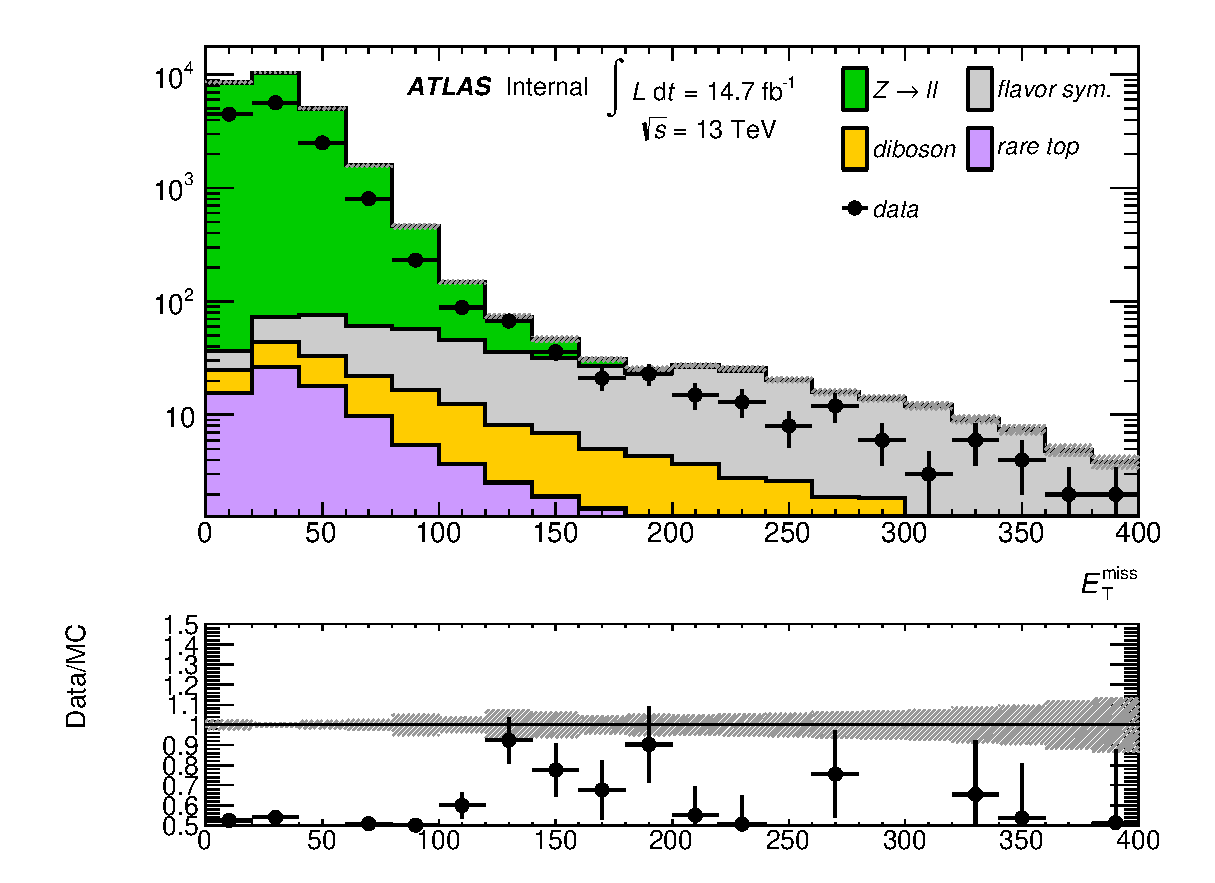
\includegraphics[width=.85\linewidth]{figures/fs/ttbar_met_dependence.eps}
\caption{Comparison of data and \ac{MC} in a selection like SRZ, without the \met cut.}
\label{fig:fs_mc_met}
\end{figure}
\end{centering}

This method is extremely effective as a crosscheck because it uses a completely independent dataset from the flavor symmetry method, and the two methods have very little overlap in dependence on \ac{MC}. They produce consistent results in both SRZ and VRS, as shown in \autoref{tab:fs_comparison}.


\begin{table}[h]
\centering

\begin{tabular}{ccc}
\noalign{\smallskip}\hline\noalign{\smallskip}
Region  & Flavour-symmetry  & Sideband fit  \\
\noalign{\smallskip}\hline\noalign{\smallskip}
SRZ & $33 \pm 4$   &  $29 \pm 7$  \\ [+0.05cm]
VR-S & $99\pm8$        &  $92 \pm 25$  \\ [+0.05cm]
\noalign{\smallskip}\hline
\end{tabular}
\caption{ Comparison of \ac{FS} background predictions from the nominal method, the flavor symmetry method, and the cross-check, the sideband fit method. Uncertainties include statistical and systematic uncertainties in both cases. }
\label{tab:fs_comparison}
\end{table}

\section{\dyjets Background}
\label{sec:bg-z}

\section{Fakes}
\label{sec:bg-fake}

The fakes background consists of processes that produce only one lepton, but whose events are otherwise kinematically similar to the \ac{SR}. These processes include semileptonic \ttbar, $W$+jets processes, and single top. Though these processes typically only produce one lepton, they can be reconstructed with two leptons due to a hadron being misidentified as a lepton or from real non-prompt lepton resulting from photon conversions or $b$-hadron decays. As such, it includes both events that have been properly reconstructed and many that are included in the \ac{SR} due to imperfect reconstruction. As with the \dyjets background, it is very difficult to predict with \ac{MC} because the flaws in reconstruction are typically less well described by the models used in \ac{MC} production than the successes. Nonetheless, a rough estimate can be made of this background by using \ac{MC}, which indicates that the number of fake events in SRZ is consistent with zero. 

Despite the small predicted contribution in the \ac{SR}, a data-driven method called the ``matrix method'' is employed to estimate these fake events \cite{SUSY-2013-20}. This method is also used to estimate the fakes contribution to other control and validation regions where their effect is often more significant. 

In the matrix method, the quality requirements for signal leptons are loosened to give a selection of baseline leptons (see \autoref{tab:eledef} and \autoref{tab:muondef}), which consist of a higher fraction of fake leptons. In each CR, VR, or SR, the remaining kinematic selections are made on the baseline leptons, and the number of leptons in that region which pass the signal lepton requirements ($N_{pass}$) and the number which fail ($N_{fail}$) are measured. For a 1-lepton selection, these quantities can be used to predict the number of fake events that pass the selection according to:

\begin{equation}
N_{\text{pass}}^{\text{fake}} = \frac{N_{\text{fail}} - (1/\epsilon^{\text{real}} - 1) \times N_{\text{pass}} }{1/\epsilon^{\text{fake}} - 1/\epsilon^{\text{real}}}.
\end{equation}

The efficiencies $\epsilon^{real}$ and $\epsilon^{fake}$ give the relative identification efficiency from baseline to signal for genuine, prompt leptons and fake and non-prompt leptons, respectively. For a 2-lepton selection, the principle is the same, but the equation is more complicated, and it requires four-by-four matrix to account for possible combinations of real and fake leptons. 


To calculate $\epsilon^{real}$, the tag-and-probe method is performed a selection of $Z\rightarrow\ell\ell$ data events, CR-real, described in \autoref{tab:regions-fakes}. In this method, one ``tag'' lepton passing a signal selection is required, as is another ``probe'' lepton passing a baseline requirement. Distributions of \mll for tag + passing probe and tag + failing probe are then fit, and the efficiency is computed using the ratio acquired from the fit. A comparison of data and \ac{MC} in CR-real can be seen in \autoref{fig:fake_realreg}.
 
\begin{table}[htbp]

\resizebox{1\textwidth}{!}{
 \begin{tabular}{lccccccc} %{\textwidth}{@{\extracolsep{\fill}}lcccccccc}
   \noalign{\smallskip}\hline\noalign{\smallskip}
     {\bf Fakes }   &  {\bf \met}   & {\bf $\HT$}  &  {\bf $n_{\text{jets}}$}  & {\bf $m_{\ell\ell} $} &  {\bf SF/DF}  & {\bf OS/SS} & $n_\ell$\\
     {\bf regions} &  {\bf [\GeV]} & {\bf [\GeV]} &                           & {\bf [\GeV]}          &               &         & \\
   \noalign{\smallskip}\hline\noalign{\smallskip}
   CR-real          &  $-$      &  $\bm{> 200}$  &  $\geq 2$ & {\bf 81--101}    &  $2\ell$ SF  & OS & $2$\\
   CR-fake          &  $\bm{<125}$   &  $-$      &  $-$ & $>12$     &  {\bf $2\ell$ SF/DF}  & {\bf SS} & $\geq2$\\
   \noalign{\smallskip}\hline\noalign{\smallskip}
   \noalign{\smallskip}\hline\noalign{\smallskip}
\end{tabular}
} % end of resizebox
\begin{center}
 \caption{Control regions used to measure efficiencies of real and fake leptons. 
 The flavour combination of the dilepton pair is denoted as either ``SF'' for same-flavour or ``DF'' for different flavour.
The charge combination of the leading lepton pairs are given as ``SS'' for same-sign or ``OS'' for opposite-sign.}
\label{tab:regions-fakes}
\end{center}
\end{table}

\begin{centering}
\begin{figure}[bth]
\myfloatalign
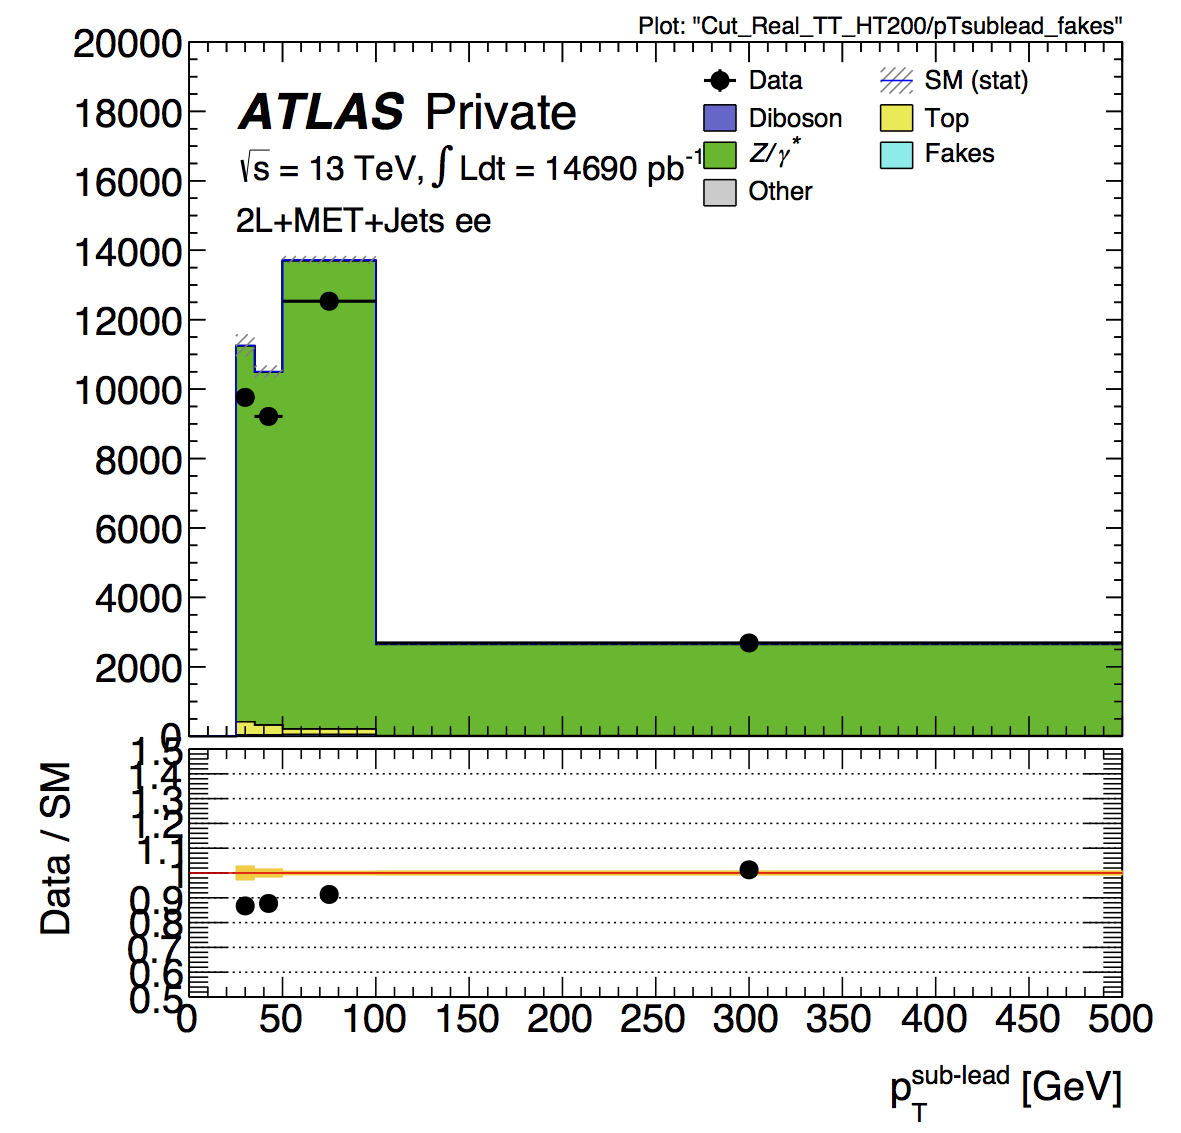
\includegraphics[width=.45\linewidth]{figures/fakes/ee-Cut_Real_TT_HT200-pTsublead_fakes-lin_2016.png}
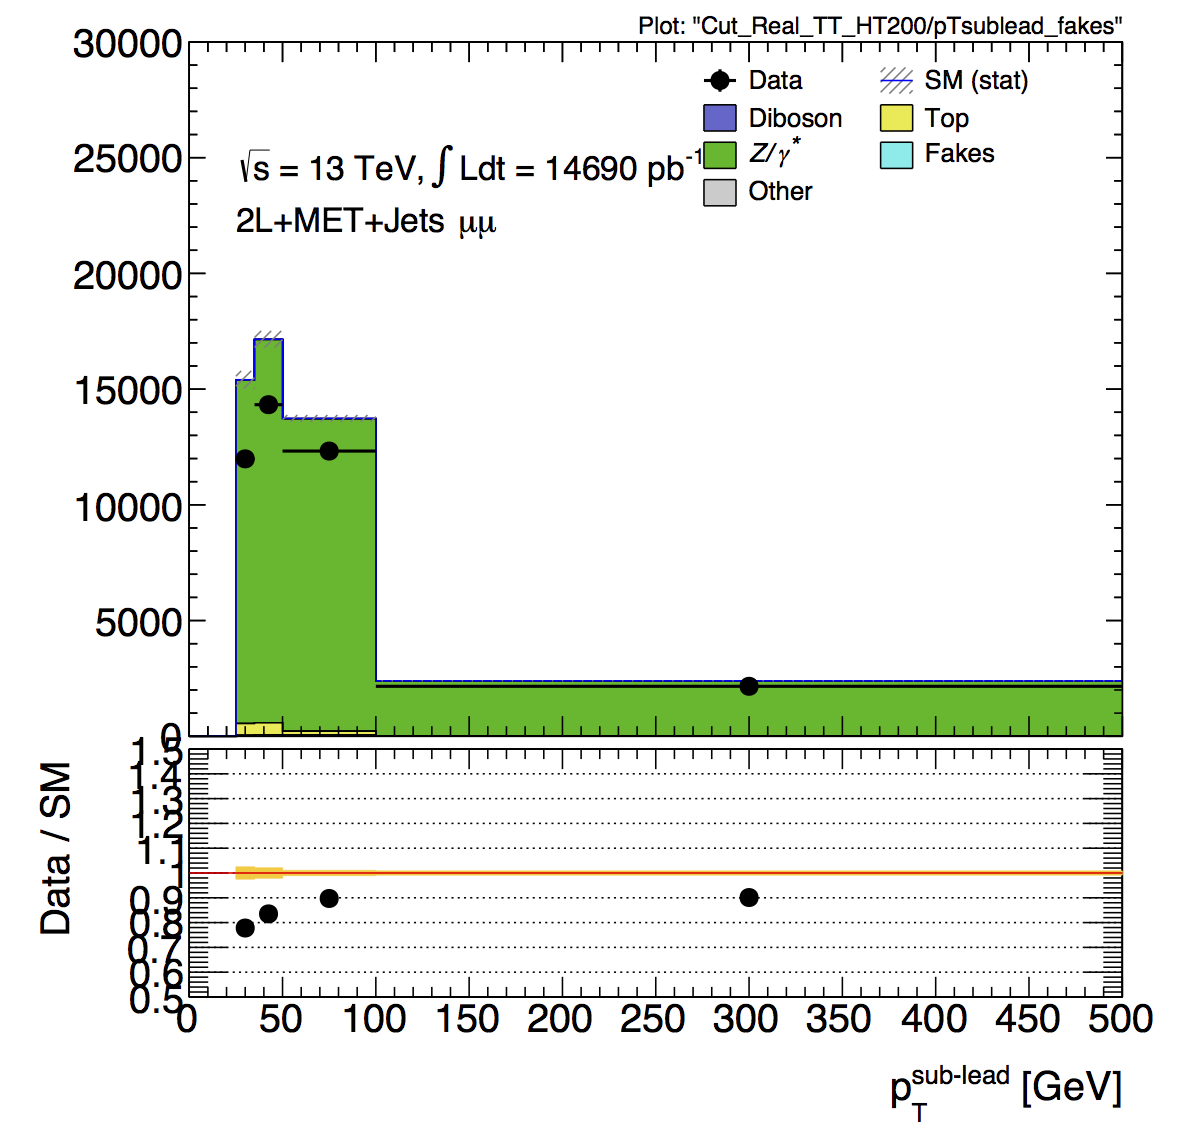
\includegraphics[width=.45\linewidth]{figures/fakes/mm-Cut_Real_TT_HT200-pTsublead_fakes-lin_2016.png}
\caption{Sub-leading lepton \pT\ for $ee$ (left) and $\mu\mu$ (right) events in the tight-tight region used to measure the real-lepton efficiency for 2016. }
\label{fig:fake_realreg}
\end{figure}
\end{centering}

The fake efficiency, $\epsilon^{fake}$, is determined using the tag-and-probe method in CR-fake, also described in \autoref{tab:regions-fakes}. This region is different from all other regions considered in this analysis because it requires same-sign leptons. Very few processes genuinely produce two same-sign leptons, so this region is enhanced in fake leptons. An upper limit on \met is placed on CR-fake to limit the possible contamination from \ac{BSM} processes. According to \ac{MC}, real, prompt leptons make up about 7\% (11\%) of the baseline electron (muon) sample and about 10\% (61\%) of the signal electron (muon) sample. These backgrounds are subtracted from the CR-fake yields when calculating the efficiencies. \autoref{fig:fake_fakereg} shows a comparison of data and \ac{MC} in this region.

\begin{centering}
\begin{figure}[htbp]
\centering
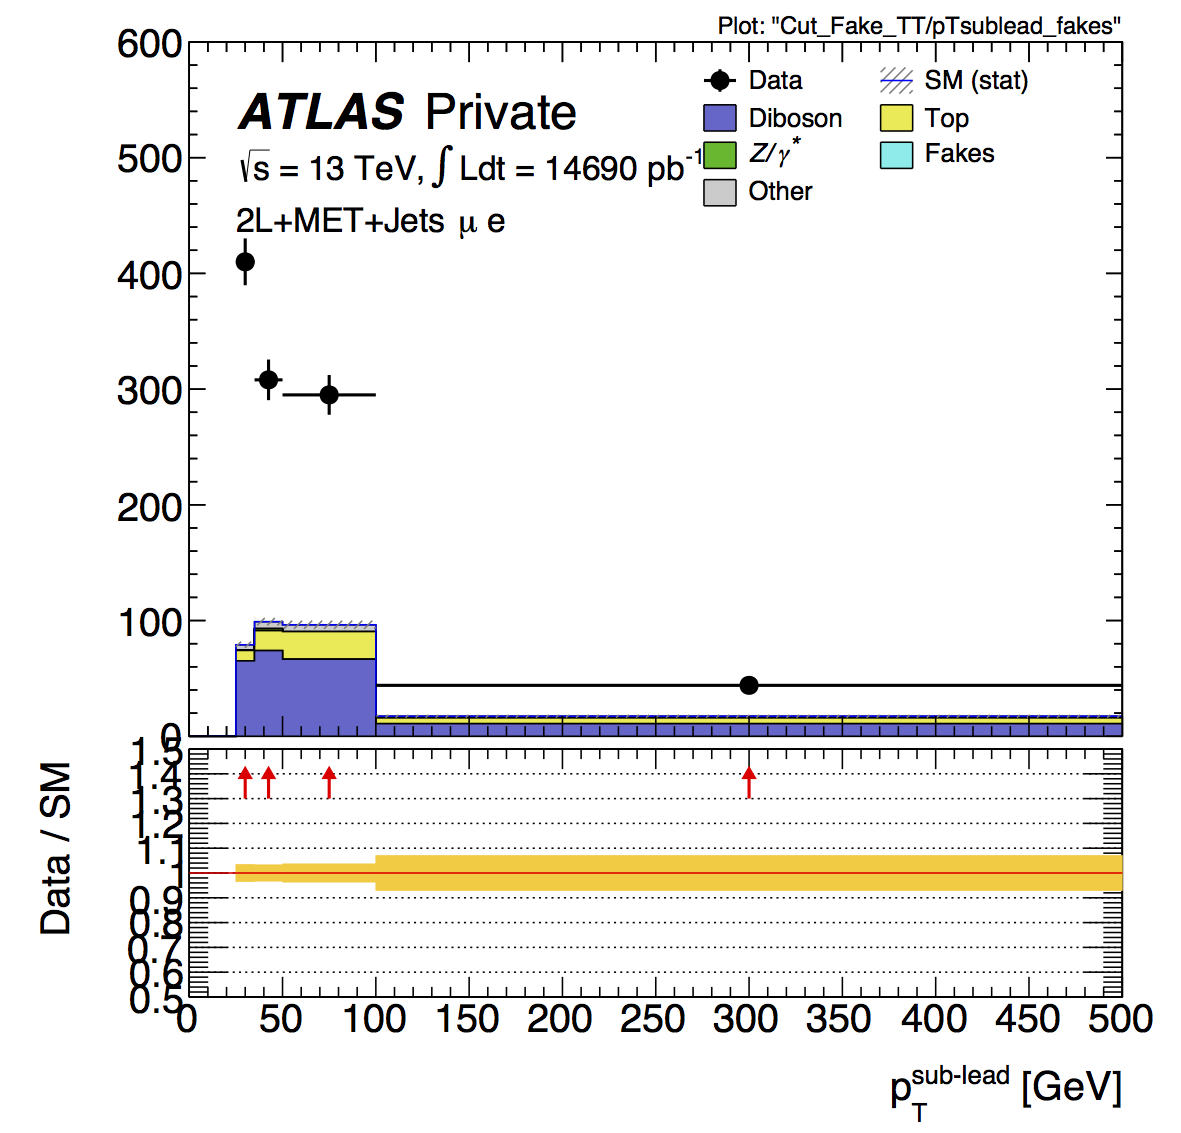
\includegraphics[width=.45\textwidth]{figures/fakes/me-Cut_Fake_TT-pTsublead_fakes-lin_2016.png}
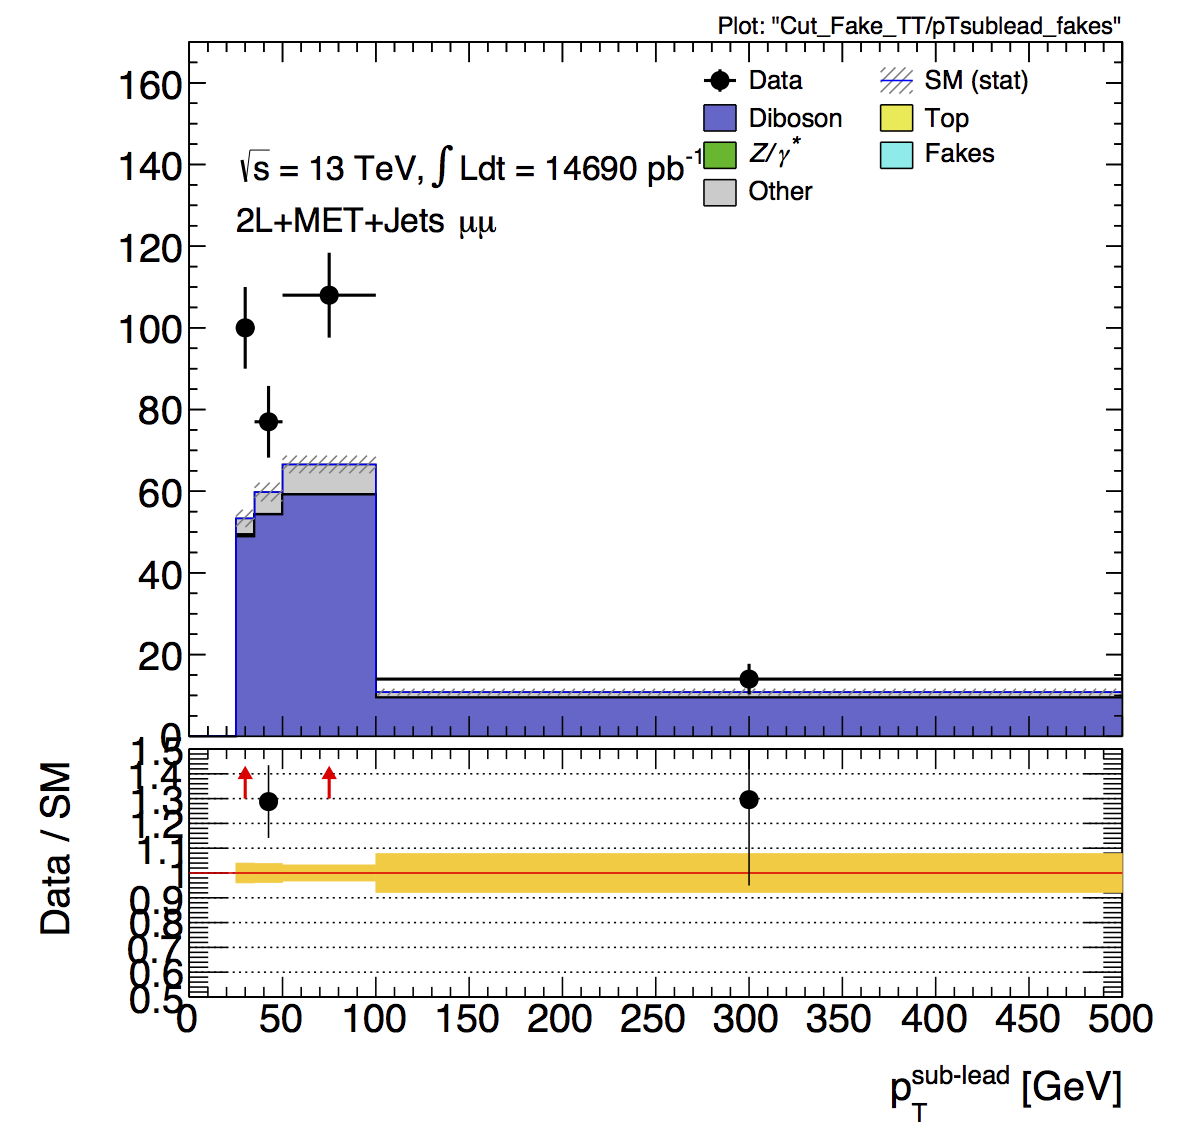
\includegraphics[width=.45\textwidth]{figures/fakes/mm-Cut_Fake_TT-pTsublead_fakes-lin_2016.png}
\caption{Sub-leading lepton \pT\ for $\mu e$ (left) and $\mu\mu$ (right) events in the tight-tight region used to measure the fake-lepton efficiency for 2016.}
\label{fig:fake_fakereg}
\end{figure}
\end{centering}

This method is validated in a fakes-rich validation region with a same-sign lepton requirement, \met$\geq$50\gev, $\geq$2 jets, and a veto on \mll on the $Z$-mass peak for same flavor channels. The results of this validation can be seen in \autoref{fig:fakes_validation}. With the systematic uncertainties included, the prediction agrees well with the data across a wide range of \mll values. 

\begin{figure}[htbp]
\centering
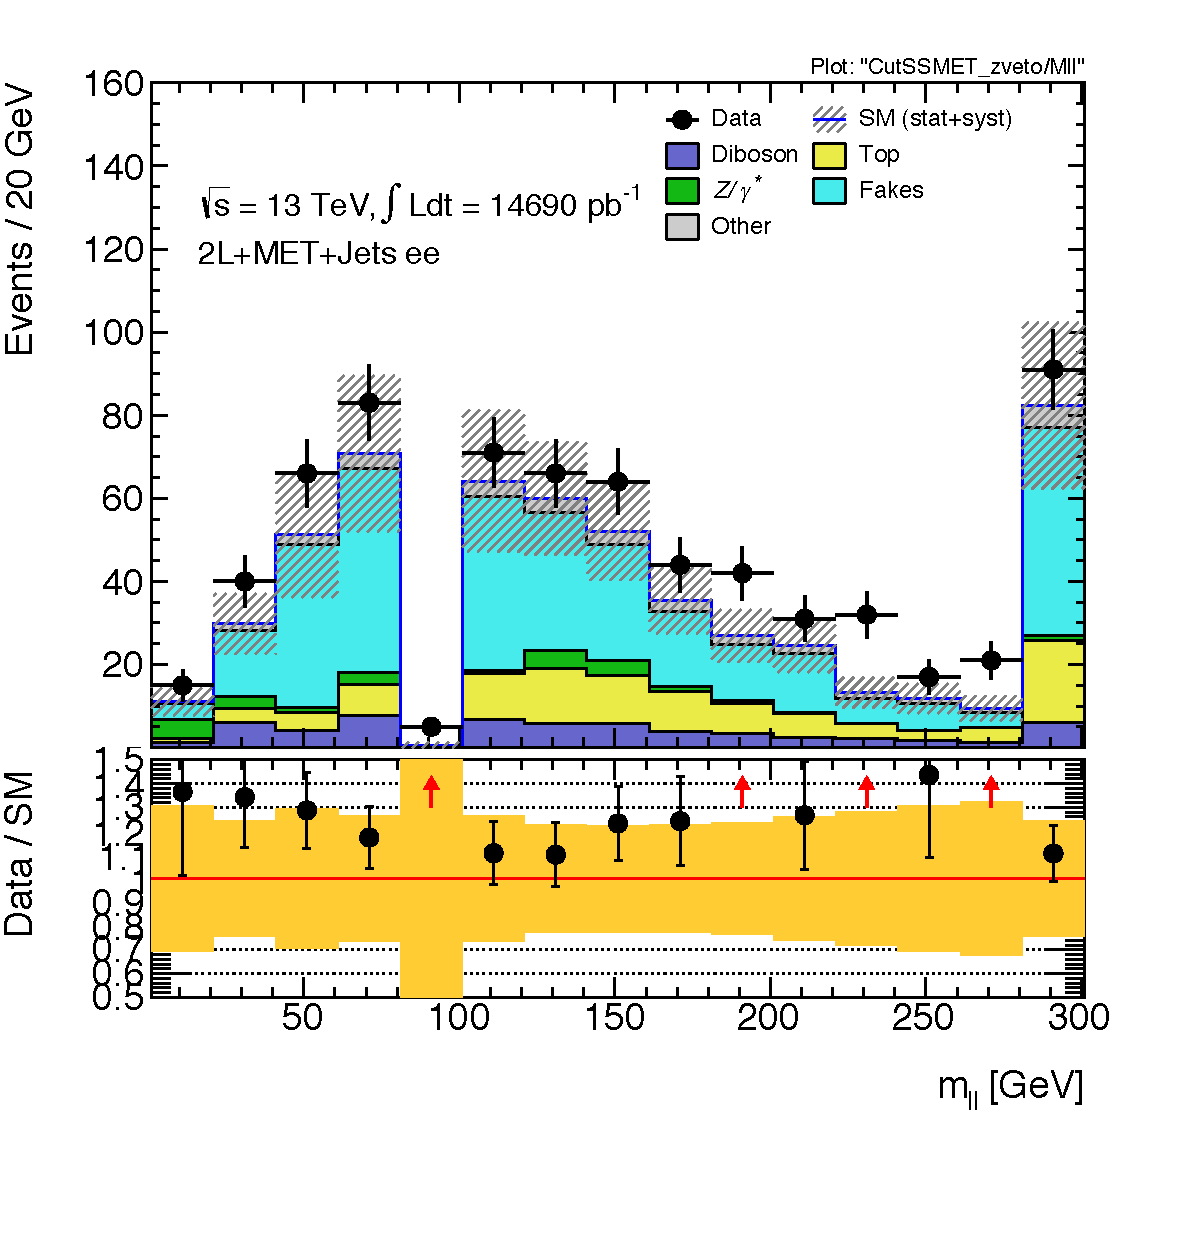
\includegraphics[width=.45\textwidth]{figures/fakes/ee-CutSSMET_zveto-Mll-lin.pdf}
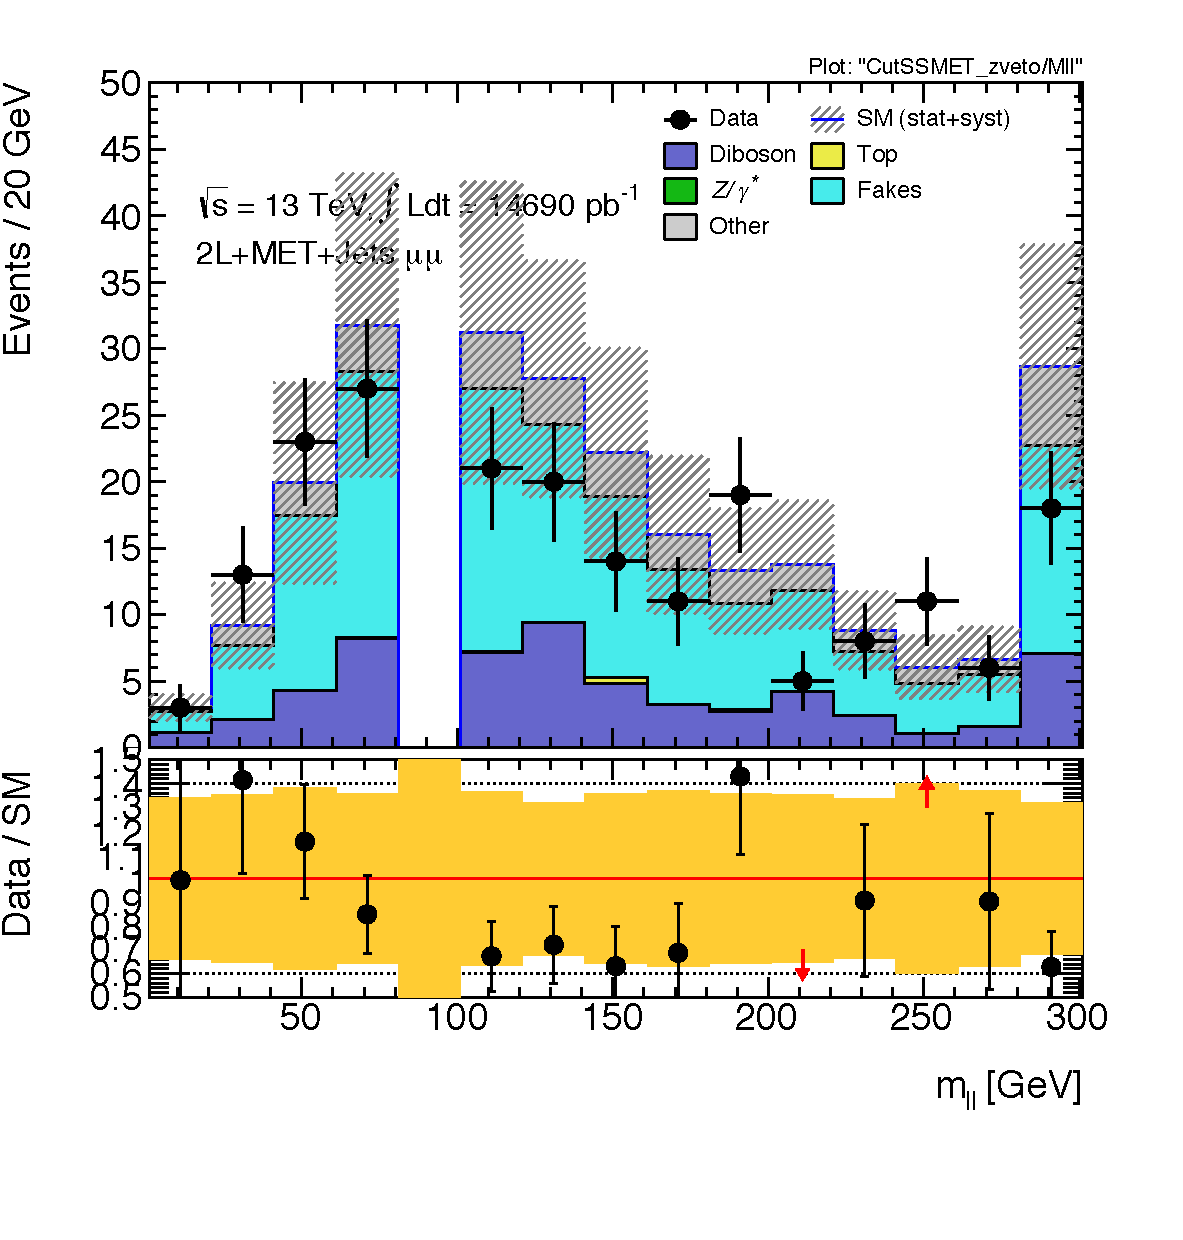
\includegraphics[width=.45\textwidth]{figures/fakes/mm-CutSSMET_zveto-Mll-lin.pdf}
\includegraphics[width=.45\textwidth]{figures/fakes/em-CutSSMET_zveto-Mll-lin.pdf}
\includegraphics[width=.45\textwidth]{figures/fakes/me-CutSSMET_zveto-Mll-lin.pdf}
\caption{Same sign validation regions in the $ee$ (top left), $\mu\mu$ (top right), $e\mu$ (bottom left) and $\mu e$ (bottom right) channels combining 2015+2016 data. Uncertainty bands include both statistical and systematic uncertainties. \label{fig:fakes_validation}}
\end{figure}


\section{Diboson and Rare Top Processes}
\label{sec:bg-other}

The remaining backgrounds are diboson processes (excluding $WW$, which is included in the \ac{FS} background) and rare top processes. Dibosons events make up about 30\% of the events in SRZ, while rare top process contributions are much smaller. Both are taken directly from \ac{MC}, with validation regions to confirm the accuracy of the prediction. These regions are \autoref{tab:regions-z}, and target different parts of these backgrounds. VR-ZZ is a four-lepton selection designed to select a very pure sample of $ZZ$ events. VR-WZ requires three leptons and specific cuts on $m_T$, the transverse mass, and \met in order to select mostly $WZ\rightarrow lll\nu$ events. VR-3L is similar to VR-S, but loosens the \HT and \met cuts and requires at least three leptons. This region is designed to target any $\geq3$-lepton process in a region as kinematically close to SRZ as possible while still maintaining enough events to validate. The makeups of these multilepton validation regions, as well as VRS, are shown in \autoref{tab:VRresults}.

\begin{table}
\begin{center}
\setlength{\tabcolsep}{0.0pc}
\begin{tabular*}{\textwidth}{@{\extracolsep{\fill}}lrrrr}
\noalign{\smallskip}\hline\noalign{\smallskip}
                                                                             & VR-S            & VR-WZ        & VR-ZZ          & VR-3L   \\[-0.05cm]
\noalign{\smallskip}\hline\noalign{\smallskip}
Observed events                                                              & $236$            & $698$        & $132$          & $32$ \\
\noalign{\smallskip}\hline\noalign{\smallskip}
%Total expected background events                                             & $223.92 \pm 40.84$   &   $612.97\pm8.65$   &    $139.29\pm4.95$    &    $34.52\pm1.39$ \\
% here the total background uncertainty is updated to the quadrature sum of each bkg uncertainty
Total expected background events                                             & $224 \pm 41$   &   $613\pm66$   &    $139\pm25$    &    $35\pm10$ \\
\noalign{\smallskip}\hline\noalign{\smallskip}
  Flavour-symmetric (\ttbar, $Wt$, $WW$, $Z\rightarrow\tau\tau$)             & $99\pm8$   &   -                &    -                 &    -              \\
  $WZ/ZZ$ events                                                             & $27\pm13$  &   $573\pm66$ &    $139\pm25$        &    $25\pm10$ \\
  Rare top events                                                            & $11\pm3$   &   $14\pm3$   &    $0.44\pm0.11$     &    $9.1\pm2.3$  \\
  \dyjets\ events                                                            & $84\pm37$  &   -                &    -                 &    -              \\
  Fake lepton events                                                         & $4\pm4$    &   $26\pm6$   &    -                 &    $0.6\pm0.3$  \\
 \noalign{\smallskip}\hline\noalign{\smallskip}
\end{tabular*}
\end{center}
\caption{Yields in validation regions. In VRS, data-driven background estimates are used for \dyjets, fakes, and \ac{FS} processes. All other backgrounds are taken from \ac{MC}, including all backgrounds in the multi-lepton \ac{VR}s. Uncertainties include statistical and systematic components. }
\label{tab:VRresults}
\end{table}
 % Background Estimation and Systematic Uncertainty
% Chapter 10

\chapter{Systematic Uncertainties} % Chapter title

\label{ch:background_uncertainties} 

Each background has a series of uncertainties placed on it based on the reliability of all the assumptions made in its prediction method. For data-driven backgrounds, each background has its own series of uncertainties based on the specifics of the method used. \ac{MC}-based methods have uncertainties that are more universal, including uncertainties on the theoretical models used to produce matrix elements and uncertainties on the modeling of the experimental setup. 

\section{Uncertainties on Data-Driven Backgrounds}

This section describes the uncertainties derived for each of the data-driven backgrounds methods: the flavor symmetry method, the \gjets prediction of the \dyjets background, and the matrix method applied to the fakes background.  

\subsection{Uncertainties on the Flavor Symmetry Method}
\label{sec:unc_fs}

The flavor symmetry method is a data driven method that makes its estimate primarily on based events populating a \ac{CR} in the different-flavor channel. The statistical uncertainty on these events makes up the dominant uncertainty on the method. To reduce this uncertainty, the \mll~range for the \ac{CR} is expanded, approximately tripling the number of events in CR-FS. The statistical uncertainty is reduced by this expansion, though it is still significantly higher than any of the other systematic uncertainties on this method, as seen in \autoref{tab:fs_errors}. Also included in the statistical uncertainty column is the statistical uncertainty on the number of non-\ac{FS} events in CR-FS, which is used to scale the prediction to account for contamination in the \ac{CR}. 

\begin{table}[!ht]
\begin{center}
 \begin{tabular}{lcc|cccccc}
 \hline 
 \multirow{3}{*}{Reg.}	& \multirow{3}{*}{Ch.} 	& \multirow{3}{*}{Pred.} & \multicolumn{6}{c}{Uncertainties} \\
   \cline{4-9} 
   		 	& 		 	& 	  		& stat.  		& MC 		& k  			& dAOD 		& \mll  	& total \\
   			& 			& 		 	& 			 	& clos. 	& and $\alpha$	& usage	 	& shape  	& \\
   \hline
   \hline
\multirow{3}{*}{SRZ}
& $ee$            & 16.5 & 1.8 & 0.88 & 0.53 & 0.12 & 0.22 & 2.1 \\ 
& $\mu\mu$        & 16.7 & 1.8 & 0.79 & 0.33 & 0.11 & 0.23 & 2.0 \\ 
& $ee$+$\mu\mu$   & 33.2 & 3.7 & 1.1 & 0.86 & 0.23 & 0.45 & 4.0 \\ 
\hline
\multirow{3}{*}{VRS}
& $ee$            & 49.7 & 3.2 & 2.3 & 2.2 & 0.34 & 0.75 & 4.6 \\ 
& $\mu\mu$        & 49.6 & 3.1 & 2.9 & 1.4 & 0.31 & 0.75 & 4.6 \\ 
& $ee$+$\mu\mu$   & 99.3 & 6.3 & 4.0 & 3.6 & 0.65 & 1.5 & 8.5 \\ 
\hline
 
\hline
\hline
 \end{tabular}
\end{center}
 \caption{
   Uncertainties on the prediction of flavor symmetric events in SRZ and VRS. Nominal predictions are given with statistical uncertainty (including uncertainty from subtracted backgrounds), MC Closure uncertainty, uncertainty on the prediction from varying $k$ and $\alpha$ by their statistical uncertainties, comparing the efficiencies from AODs to that of DAODs, and on the \mll~widening, which includes MC statistics and a data/MC comparison in a loosened region.
 }
 \label{tab:fs_errors}
\end{table}

The next largest contribution to the uncertainty comes from \ac{MC} closure tests, which are used to determine how effective the method is in its prediction. If, for example, using weights derived from an inclusive selection at high \met lead to a bias, the closure test would indicate that and an appropriate uncertainty could be placed on the estimate based on the difference between the \ac{MC} prediction and the prediction from the flavor symmetry method. 

In this test, the entire \ac{FS} procedure is performed on \ttbar \ac{MC}, including a recalculation of weighting factors $\alpha$ and $k$. The prediction from $e\mu$ events in \ac{MC} is compared to the \ac{MC} $ee$ and $\mu\mu$ events, as seen in \autoref{fig:fs_closure}. The difference between the two predictions is then summed in quadrature with the statistical uncertainty on each prediction to give the total closure uncertainty seen in \autoref{tab:fs_errors}. In these closure tests, all predictions agree within the statistical uncertainty, so the largest contributor to the resulting error is \ac{MC} statistics. In SRZ, the total statistical uncertainty on the closure corresponded to 1.06 events, while the uncertainty due to the difference between the estimates was only 0.13 events. 

\begin{centering}
\begin{figure}[!hbt]
\myfloatalign
\includegraphics[width=.85\linewidth]{figures/fs/ee+mm_ratio_mll_VRZ_widened.eps}
\includegraphics[width=.85\linewidth]{figures/fs/ee+mm_ratio_mll_SRZ_widened.eps}
\caption{\ac{MC} closure plots of VRS (top) and SRZ (bottom). The number of events from MC (black points) is compared to the number of events predicted from the flavor symmetry method (yellow histogram). The figure shows the comparison before $f_{Z \mathrm{\text{-}mass}}$ is used to make convert the wider \mll~range into an on-$Z$ prediction, but because $f_{Z \mathrm{\text{-}mass}}$ is taken from \ac{MC}, the result is identical.}
\label{fig:fs_closure}
\end{figure}
\end{centering}

A small uncertainty is added based on the statistical uncertainty on the $k$ and $\alpha$ factors derived from data. These factors are measured in many different bins (see, for example, the different measurements of $k$ in \autoref{fig:fs_k}), and as a consequence, some bins can have very large statistical uncertainties. To assess the uncertainty on the total estimate, each measurement of these factors is varied by its uncertainty in order to produce the maximum and minimum possible prediction. The differences with respect to the nominal prediction are used to create a symmetrized error, which is included in \autoref{tab:fs_errors}.

The next uncertainty considers a potential bias in the way the $\alpha$ factors are calculated. Because they are derived from data, there is already trigger dependence in data collection; only events passing a trigger are stored. Additional trigger dependence is created by the data format used for analysis. \ac{ATLAS} data and \ac{MC} are stored in a format called \ac{AOD}, but smaller, slimmed versions of these datasets, called \acp{dAOD} are used for analysis. These \acp{dAOD} are designed with specific analyses in mind, and in a processes called \textit{skimming}, are filtered based on the triggers and objects required by the analyses. As a consequence, in the \ac{dAOD} used in this analysis, there are explicit requirements that lepton or \met triggers are passed in order for events to be included. 

As a consequence, the trigger efficiencies $\epsilon^\text{trig}$ used in \autoref{eq:kandalpha} to define $\alpha$ do not consider all possible data events. The $\epsilon^\text{trig}$ factor is calculated for each trigger using events passing the kinematic selection for that trigger, outlined in \autoref{sec:trig_strategy}. The efficiency factor is then measured according to the equation
%
\begin{equation}
\epsilon^\text{trig} = \frac{N_\text{trig}}{N_\text{all}} , 
\end{equation}
%
where $N_\text{trig}$ is the number of events passing the trigger in the kinematic selection and $N_\text{all}$ is all events in the selection. The latter measurement is the one subject to this bias, as it contains only the events that pass at least one trigger required for inclusion in the \ac{dAOD}. As a consequence of these missing events, the $\epsilon^\text{trig}$ values will be artificially high. However, because the ratio of trigger efficiencies for the different channels is the only quantity needed for this analysis, the missing events will only bias the prediction if the different channels are differently impacted by the trigger preselection.

Calculating the flavor symmetry method's dependence on these biases requires the use of \ac{MC}. With a generated \ac{MC} sample, there is no trigger dependence, so an unskimmed sample can be compared to a typical skimmed \ac{MC} \ac{dAOD} to identify the effect of the skimming. \autoref{fig:fs_alpha} shows a comparison of the $\alpha$ factors calculated for different bins in \met from the nominal source, data, as well as these two \ac{MC} selections. 

\begin{centering}
\begin{figure}[!hbt]
\myfloatalign
\includegraphics[width=.85\linewidth]{figures/fs/trigger_ratios.eps}
\caption{$\alpha$, the trigger efficiency ratio, calculated as a function of \met from three different sources: data (blue), the usual skimmed \ttbar \ac{MC} (red), and an unskimmed \ttbar \ac{MC} (green).}
\label{fig:fs_alpha}
\end{figure}
\end{centering}

An \met dependence would be the most likely bias between the two \ac{MC}-derived $\alpha$ factors because \met triggers are the only triggers besides lepton triggers that will allow an event to be accepted into the \ac{dAOD} used by this analysis. Though there is some difference between the data-derived $\alpha$ and those taken from \ac{MC}, it is clear from this plot that there is very little dependence on the choice of an unskimmed or skimmed sample. The calculation of the uncertainty is performed by repeating the flavor symmetric method in \ac{MC} with each of the two \ac{MC}-based $\alpha$ factors and using the difference between the estimates as a symmetric error.

The last uncertainty relates to the main \ac{MC} dependence of the method - the \mll~shape of the \ac{FS} background. A correction factor is taken from \ac{MC} in order to account for the \mll~widening, and the accuracy of that factor must be checked. Its shape is compared to that of data in a region similar to VR-FS, but with an \HT cut lowered to 300 \gev~to increase statistics. The difference between the fraction of events on the $Z$-mass peak in data and \ac{MC} in this region is taken as a systematic uncertainty. To confirm that using this lowered \HT cut still gives a valid answer, the fractions are compared as a function of \HT in \autoref{fig:fs_frac_ht}. In these plots, especially in the higher-statistics 2016 plot, it is clear both that the data and \ac{MC} agree very well and that there is no strong \HT dependence. 

\begin{centering}
\begin{figure}[!hbt]
\myfloatalign
\includegraphics[width=.85\linewidth]{figures/fs/frac_vs_ht_2015.eps}
\includegraphics[width=.85\linewidth]{figures/fs/frac_vs_ht_2016.eps}
\caption{Plots of the fraction of on-Z events with a VR-FS-like selection as a function of \HT for data and \ttbar \ac{MC}. The top figure shows 2015 data and \ac{MC} while the bottom figure shows the same for 2016.}
\label{fig:fs_frac_ht}
\end{figure}
\end{centering}

All the uncertainties are calculated independently for the 2015 and 2016 datasets, then added together. Statistical uncertainties, including the \ac{MC} closure statistical uncertainties and the $k$ and $\alpha$ uncertainties, are added in quadrature between the two years. Uncertainties that are more likely to be correlated, such as the difference between the two estimates in \ac{MC} closure and the dependence on using a dAOD to calculate trigger efficiencies, are added linearly. The total uncertainty is about 12\% of the nominal prediction in SRZ and about 9\% in VRS. 

%----------------------------------------------------------------------------------------

\subsection{Uncertainties on the \gjets Method}
\label{sec:unc_gjets}

One of the largest sources of uncertainty on the \gjets method is derived by comparing the results from reweighting in different variables. Though boson \pt is used as the nominal reweighting variable, the differences in the kinematics of $\gamma$ and $Z$ events also impact number of jets, \HT, and $E_{\text{T}}$ (which includes the mass of the boson). The \gjets method is repeated using each of these variables to reweight, and their \met distributions are shown in \autoref{fig:photons_rwunc}. The maximum difference from the nominal prediction is symmetrized and used as an uncertainty on the method. 

\begin{centering}
\begin{figure}[bth]
\myfloatalign
\includegraphics[width=.85\linewidth]{figures/photons/GJ_Variations_ee+mm_zmet_onz.pdf}
\caption{\met distributions for \gjets predictions using different reweighting variables, as well as distributions with the nominal reweighting but with smearing functions taken from data and from \ac{MC} in a $\geq$2-jet region.}
\label{fig:photons_rwunc}
\end{figure}
\end{centering}

Another uncertainty is applied to estimate the validity of using \ac{MC} in a 1-jet \ac{CR} to determine the smearing functions. Smearing functions are made using data from the same 1-jet region and using \ac{MC} in a $\geq$2-jet region otherwise identical to the 1-jet \ac{CR}. These distributions are also shown in \autoref{fig:photons_rwunc}, and like the alternate reweighting distributions, are used to find a maximum difference from the nominal prediction which is translated into a symmetric error. 

As in the flavor symmetric method, the full procedure is carried out on \ac{MC} in order to test \ac{MC} closure, including a recalculation of any weights that are typically derived from data. The resulting comparison between \dyjets \ac{MC} and the \gjets method performed on \ac{MC} can be seen in \autoref{fig:photons_mcclos}. The final non-closure uncertainty is taken from VRS, where larger numbers of events give a clearer picture of the success of the method than in SRZ. In VRS, the statistical uncertainty on the prediction is compared to the non-closure, and the larger of the two is used as the final uncertainty. 

\begin{centering}
\begin{figure}[!hbt]
\myfloatalign
\includegraphics[width=.48\linewidth]{figures/photons/Closure_plot_ee_zmet.eps}
\includegraphics[width=.48\linewidth]{figures/photons/Closure_plot_mm_zmet.eps}
\caption{\ac{MC} closure of the \gjets method as a function of \met comparing the \ac{MC} prediction of the $Z$ background with the \gjets method performed on \gjets \ac{MC} in the $ee$ channel (left) and $\mu\mu$ channel (right). The uncertainty band includes both statistical and reweighting uncertainties \cite{this_paper}.}
\label{fig:photons_mcclos}
\end{figure}
\end{centering}

The uncertainty on the $V\gamma$ contamination in CR-$\gamma$ is also considered. An uncertainty on the \ac{MC} prediction is made based on comparison of data and \ac{MC} in a $W +$ jets \ac{VR}, shown in \autoref{fig:photons_vgunc}. This \ac{VR} is similar to CR-$\gamma$, but instead of vetoing events with leptons, requires at least one well-isolated lepton with a \pt over 25 \gev. At \met values over 100 \gev, the region is about 90\% pure in $W\gamma$ processes. The \ac{MC} agrees well with data in this region, even at very high \met, so an uncertainty of 16\% based primarily on statistical uncertainty in this \ac{VR} is placed on the $V\gamma$ \ac{MC}. This uncertainty is propagated to the final result through the subtraction procedure.

\begin{centering}
\begin{figure}[!hbt]
\myfloatalign
\includegraphics[width=.9\linewidth]{figures/photons/hPhotLep_mT_MET100_hist.eps}
\includegraphics[width=.9\linewidth]{figures/photons/hPhotLep_mT_MET200_hist.eps}
\caption{Distributions of $m_{\text{T}}(\ell,\met)$, the transverse mass of the lepton and the \met in a \ac{VR} designed to target $W\gamma$ processes. Top is the distribution with an \met cut at 100 \gev, and bottom is the same distribution with an \met cut of 200 \gev.}
\label{fig:photons_vgunc}
\end{figure}
\end{centering}

An uncertainty on the \mll~shape is determined using \ac{MC} closure as well. The comparison of \mll~shapes in \dyjets \ac{MC} and the \gjets method applied to \ac{MC} is shown in \autoref{fig:photon_mll_mc}. As with the main \ac{MC} closure test, the maximum of the statistical uncertainty and the non-closure is taken as the final uncertainty on this background.

One last uncertainty based on the statistical uncertainty on the number of \gjets data events used for this method is also included. The full breakdown of uncertainty in SRZ can be seen in \autoref{tab:photon_uncertainties}. The final uncertainty is nearly 100\%.

\begin{table}[!hbt]
\centering
\resizebox{\textwidth}{!}{

 \begin{tabular}{cc|ccccccc}
 \hline 
\multirow{3}{*}{Ch.} 	& \multirow{3}{*}{Pred.} & \multicolumn{7}{c}{Uncertainties (\%)} \\
   \cline{3-9} 
   		 	& 	  		& $V\gamma$ 	& MC  		& \mll 	& re- 		& smear  & stat.  	& total \\
   			& 		 	& sub. 			& clos.		& shape & weight	& 		 & 	 		& \\
   \hline
   \hline
$ee$ 			& 1.0        & 53 & 21 & 19 & 100 & 65 & 56 & 145 \\ 
$\mu\mu$ 		& 2.1     & 27 & 14 & 23 & 30  & 59 & 40 & 86 \\ 
$ee$+$\mu\mu$ 	& 3.1     & 36 & 16 & 22 & 43  & 60 & 33 & 92 \\ 
 

\hline
\hline
 \end{tabular}
}
\caption{Uncertainty breakdown for the \gjets method in SRZ. Uncertainties considered are the impact of \ac{MC} uncertainty on $V\gamma$ backgrounds, \ac{MC} closure, uncertainty on \mll~shape (also determined via \ac{MC} closure), reweighting uncertainties, smearing uncertainties, and statistical uncertainty on the \gjets events used in the method.}
\label{tab:photon_uncertainties}
\end{table}

%----------------------------------------------------------------------------------------

\subsection{Uncertainties on the Fakes Background}
\label{sec:uncert_fakes}

Systematic uncertainties on the fakes background are derived from a series of variations on the nominal method.  Variations include scaling the real and fake efficiencies up and down by their statistical uncertainties, scaling the prompt lepton contamination in CR-fake up and down by 20\%, and by requiring and vetoing $b$-tagged jets in CR-fake to determine the dependence on heavy flavor. 
Statistical uncertainties can also be large in regions with small numbers of events in the the baseline selection, such as SRZ. In other regions, the $b$-tagging dependence provides the largest uncertainty. The full breakdown of uncertainties for the most important regions are listed in ~\autoref{tab:syst:fakes_onz1516}.

\begin{table}[!hbt]
\centering
\resizebox{\textwidth}{!}{
\begin{tabular}{l|cccccc}
Variation & SRZ & CRT & CRFS & VRFS & VRS & VRT  \\
\hline\hline
Nominal & 0.10 $\pm$ 1.61 & 25 $\pm$ 5 & 3.7 $\pm$ 2.2 & 11 $\pm$ 4 & 3.6 $\pm$ 3.2 & 80 $\pm$ 10   \\
\hline
EL F Up     & 0.15  	& 30 & 4.0 & 11 & 3.6  	& 92   \\
EL F Down   & 0.06  	& 22 & 3.5 & 10 & 3.5 	& 70   \\
EL R Up     & 0.25  	& 26 & 3.9 & 11 & 4.1 	& 83   \\
EL R Down   & -0.07  & 25 & 3.5 & 10 & 3.1 	& 77   \\
MU F Up     & -0.20  & 32 & 4.8 & 16 & 5.3 	& 86   \\
MU F Down   & 0.29  	& 20 & 2.9 & 7.0 & 2.9 	& 70   \\
MU R Up     & 0.13 	& 26 & 3.8 & 11 & 3.8 	& 81   \\
MU R Down   & 0.05 	& 25 & 3.7 & 10 & 3.4 	& 79   \\
\hline
Total Sys 		   & +0.26 -0.35 		 & +8.6 -6.4 	  & +1.1 -0.87 	& +5.9 -3.6 	 & +1.7 -0.97  	& +14 -14  \\
Total Sys (\%) 	& +261 -355  & +34 -25    & +29 -23 & +56 -34 & +47 -27  & +18 -18  \\
\hline
Real Cont. Up 	& 0.23 	& 21 & 3.1 & 8.1 	& 3.2 & 69   \\
Real Cont. Down & -0.01 & 30 & 4.4 & 13 	& 4.2 & 90   \\
b-jet 			& 0.31 	& 40 & 5.3 & 9.0 	& 5.6 & 121   \\
no b-jet 		& 0.16 	& 23 & 3.1 & 11 	& 4.0 & 71   \\
\hline
Total Sys      & +0.25 -0.11 			& +16 -4.8 & +1.7 -0.93 & +2.6 -2.9 & +2.1 -0.49  			& +42 -15  \\
Total Sys (\%) & +260 -109 	& +62 -19 & +45 -245 & +24 -28 & +57 -13 	& +52 -18  \\
\hline\hline
\end{tabular}
}
\caption{ Systematic uncertainties on the fake-lepton background for on-Z regions for 2015+2016 yields. The nominal yield includes statistical uncertainty from the baseline selection in a given region. The following rows indicate the results of varying the real and fake lepton efficiencies up and down by by their statistical uncertainty. Real cont. gives an uncertainty on the the contamination of real leptons in the fake lepton efficiency. $b$-jet and no $b$-jet indicate the impact of requiring or vetoing $b$-tagged jets in the regions used to measure the fake efficiency. \label{tab:syst:fakes_onz1516}}
\end{table}

%----------------------------------------------------------------------------------------

\section{Uncertainties on \acs{MC}-Driven Backgrounds}

Background estimates based on \ac{MC} are assigned uncertainties according to each assumption made in the \ac{MC} modeling. These uncertainties are broadly broken into two categories. Experimental uncertainties cover the modeling of the \ac{ATLAS} detector and its response functions, as well as the pile-up and luminosity provided by the \ac{LHC}. Theoretical uncertainties include uncertainties on \acp{PDF}, the calculation of matrix elements, and the discrepancies between different generators' predictions.

Experimental uncertainties cover any detector effect or \ac{LHC} condition that may not be modeled precisely correctly in \ac{MC}. For each uncertainty, a standard prescription from the \ac{ATLAS} experiment is followed. These uncertainties are applied to signal samples, as well as any backgrounds taken directly from \ac{MC}. Uncertainties are included on the following parameters:  
\begin{itemize}
\item Luminosity (2.9\%) \cite{2011lumi,2012lumi}
\item Jet energy scale \cite{ATL-PHYS-PUB-2015-015}
\item Jet energy resolution \cite{ATL-PHYS-PUB-2015-015}
\item Jet vertex tagging
\item Heavy flavor tagging
\item \met soft term \cite{ATL-PHYS-PUB-2015-023}
\item $e/\mu$ momentum scale  
\item $e/\mu$ trigger, reconstruction, and identification efficiencies
\item Pile-up
\end{itemize}

These uncertainties are applied to all \ac{MC} samples used in the analysis. This includes signal models, diboson and rare top samples for the nominal estimate, and all backgrounds taken from \ac{MC} in the sideband fit. 

Theoretical uncertainties include cross-section uncertainties, scale uncertainties, and \ac{PDF} uncertainties. For the diboson samples, the scale uncertainties, given in \autoref{table:Diboson_theoryuncert} are calculated by varying each scale up and down by a factor of two. These scales each represent a quantity that is necessary for calculating matrix elements, but doesn't necessarily correspond to a physical value. Ideally, the dependence on the scales would be small, and the choice of this non-physical quantity in the calculation wouldn't affect the final calculation. The scales are included. The renormalization scale  provides a cut-off value for the \pt of particles that are included in a Feynman diagram, but aren't present in either the initial or final state. The factorization scale gives the 

 These are combined with a 6\% cross-section uncertainty and a generator uncertainty obtained by comparing {\sc Powheg} and {\sc Sherpa} \ac{MC} yields in a given region. This generator uncertainty, shown in \autoref{table:Diboson_powhegsherpa1}, is dominant in most regions. Rare top processes are given a $13\%$ PDF and scale variation uncertainty \cite{Alwall:2014hca} and a $22\%$ cross section uncertainty \cite{Campbell:2012,Lazopoulos:2008,Garzelli:2012bn}. 

\begin{table}
	\begin{center}
 		\begin{tabular}{l|c|c|c|c|c|c|c}
		    \hline \hline 
   			\multicolumn{8}{c}{$VV \rightarrow ll\nu\nu$ Samples} \\
  	 		\hline
			&	SRZ & VRS & CRT & VRT & VRWZ & VRZZ & VR3L \\
			\hline
			resummation & 0.07 & 0.03 & 0.01 & 0.02 & 0.00 & 0.00 & 0.00 \\
			renormalization & 0.13 & 0.17 & 0.16 & 0.22 & 0.00 & 0.00 & 0.00 \\
			factorization & 0.01 & 0.01 & 0.01 & 0.03 & 0.00 & 0.00 & 0.00 \\
			total & 0.15 & 0.17 & 0.16 & 0.22 & 0.00 & 0.00 & 0.00 \\
		    \hline 
   			\multicolumn{8}{c}{$WZ \rightarrow lll\nu$ Samples} \\
  	 		\hline
			&	SRZ & VRS & CRT & VRT & VRWZ & VRZZ & VR3L \\
			\hline
			resummation & 0.07 & 0.05 & 0.13 & 0.08 & 0.02 & 0.00 & 0.01 \\
			renormalization & 0.26 & 0.20 & 0.28 & 0.21 & 0.07 & 0.00 & 0.18 \\
			factorization & 0.04 & 0.04 & 0.02 & 0.06 & 0.01 & 0.00 & 0.02 \\
			total & 0.28 & 0.21 & 0.31 & 0.23 & 0.07 & 0.00 & 0.18 \\
  	 		\hline
   			\multicolumn{8}{c}{$ZZ \rightarrow llll$ Samples} \\
  	 		\hline
			&	SRZ & VRS & CRT & VRT & VRWZ & VRZZ & VR3L \\
			\hline
			resummation & 0.27 & 1.07 & 0.01 & 0.01 & 0.06 & 0.01 & 0.53 \\
			renormalization & 0.28 & 0.26 & 0.30 & 0.60 & 0.07 & 0.04 & 0.14 \\
			factorization & 0.27 & 0.25 & 0.30 & 0.58 & 0.13 & 0.02 & 0.16 \\
			total & 0.48 & 1.13 & 0.43 & 0.84 & 0.16 & 0.05 & 0.57 \\
  	 		\hline\hline
 		\end{tabular}
	\end{center}
	\caption{Fractional uncertainties of dibosons in signal and validation regions from \sherpa scale variations.}
	\label{table:Diboson_theoryuncert}
\end{table}

\begin{table}
\begin{center}
\begin{tabular}{c|c|c|c|c|c} 
Region & \sherpa & \sherpa & {\sc Powheg} & {\sc Powheg} & \% \\
& Events/fb$^{-1}$ & Events & Events/fb$^{-1}$ & Events & Difference \\
\hline
\hline
\multicolumn{6}{c}{WZ Samples} \\
\hline
SRZ+VRZ & 5.22 & 76.72 & 3.29 & 48.30 & 37.05 \\
CRT+VRT & 1.06 & 15.58 & 0.74 & 10.91 & 29.97 \\
\hline
\multicolumn{6}{c}{WW/ZZ Samples} \\
\hline
SRZ+VRZ & 1.92 & 28.24 & 0.69 & 10.07 & 71.42 \\
CRT+VRT & 6.28 & 92.33 & 3.14 & 46.19 & 55.47 \\
\hline\hline
\end{tabular}
\end{center}
\caption{Comparison of yields in on-$Z$ and off-$Z$ regions in \sherpa and {\sc powheg} diboson MC at $14.7~\mathrm{fb}^{-1}$.}
\label{table:Diboson_powhegsherpa1}
\end{table}

Signal models have both the central value and uncertainty on cross-sections taken from an envelope of predictions using different scales and \ac{PDF} sets \cite{Kramer:2012bx}. The signal processes are calculated at \ac{NLO+NLL}; they are initially callculated at \ac{NLO} in the strong coupling constant, with additional terms from next-to-leading-logarithmic resummation of soft gluon emission \cite{Beenakker:1996ch,Kulesza:2008jb,Kulesza:2009kq,Beenakker:2009ha,Beenakker:2011fu}.


%----------------------------------------------------------------------------------------

\section{Impact of Uncertainties on the Signal Region}


The breakdown of each major uncertainty's contribution to the total uncertainty in SRZ is shown in \autoref{tab:syst}. The dominant uncertainty is the diboson generator uncertainty, followed by the statistical uncertainty from the \ac{FS} background. Uncertainties smaller than 1\% are not shown in the table. 

\begin{table}[h]
\centering
\small
\begin{tabular}{lc}
\noalign{\smallskip}\hline\noalign{\smallskip}
Source  & Relative systematic uncertainty [\%] \\
\noalign{\smallskip}\hline\noalign{\smallskip}
 & SRZ \\
\noalign{\smallskip}\hline\noalign{\smallskip}
Total systematic uncertainty & 17    \\ 
\noalign{\smallskip}\hline
$WZ/ZZ$ generator uncertainty  & 13  \\
Flavour symmetry (statistical) & 7   \\
$WZ/ZZ$ scale uncertainty      & 6   \\
\dyjets\ (systematic)          & 4   \\
Flavour symmetry (systematic)  & 3   \\
\dyjets\ (statistical)         & 2   \\
Fake-leptons                   & 1   \\
\noalign{\smallskip}\hline
\end{tabular}
\caption{
Overview of the dominant sources of systematic uncertainty on the total background estimate in the signal regions.
The values shown are relative to the total background estimate, shown in \%.}
\label{tab:syst}
\end{table}

%---------------------------------------------------------------------------------------- % Background Estimation and Systematic Uncertainty
% Chapter 11

\chapter{Results} % Chapter title

\label{ch:results} 

The results of the search can be seen in \autoref{tab:results}, which displays the expected and observed numbers of events in SRZ, both divided by channel and inclusively. The predictions and uncertainties for each background are shown, though many of these uncertainties are correlated between backgrounds, so the final uncertainty does not correspond to a simple addition in quadrature of each error. A total of sixty events are observed, with 53.5 $\pm$ 9.3 events expected. \autoref{fig:results_plot} shows the expected and observed results visually for the \ac{SR} as well as three \acp{VR}, all designed to verify the accuracy of the backgrounds taken from \ac{MC}. Excellent agreement is seen in all cases, with the largest deviation at about $1.2\sigma$ in VR-WZ.

\begin{centering}
\begin{figure}[!hbt]
\myfloatalign
\includegraphics[width=.9\linewidth]{figures/results/makeSummaryPlot_linear.eps}
\caption{Comparison of background predictions and data yields in four validation regions, as well as the signal region. Definitions of all regions can be found in \autoref{tab:regions-z}, with both rare top and fake backgrounds grouped together under the ``other'' label. The uncertainty band includes all statistical and systematic uncertainties. Below is a panel of the one-sided statistical significances of the deviations between the predicted and observed quantities for each region \cite{this_paper}.}
\label{fig:results_plot}
\end{figure}
\end{centering}

\begin{sidewaystable*}
\caption{
Number of events expected and observed in the $ee$, $\mu\mu$, and combined channels. Expected predictions include all systematic and statistical uncertainties discussed in \autoref{ch:background_uncertainties}. Also shown is the discovery $p$-value for zero signal strength ($p(s=0)$)~\cite{Baak:2014wma}, Gaussian significance, 95\% \ac{CL} observed and expected upper limits on the number of signal events ($S^{95}$), and the corresponding observed upper limit on the visible cross section ($\langle\epsilon\sigma\rangle^{95}_\text{obs}$).
}
\begin{center}
\setlength{\tabcolsep}{0.0pc}
%%
\begin{tabular*}{\textwidth}{@{\extracolsep{\fill}}lccc}
\noalign{\smallskip}\hline\noalign{\smallskip}
                                                                            & SRZ                 & SRZ $ee$      & SRZ $\mu\mu$  \\[-0.05cm]
\noalign{\smallskip}\hline\noalign{\smallskip}
%%
Observed events                                                             & $60$                     & $35$                   &   $25$ \\
\noalign{\smallskip}\hline\noalign{\smallskip}
%%
Total expected background events                                            & $53.5 \pm 9.3$         & $27.1 \pm 5.1$       &   $26.8 \pm 4.4$ \\
\noalign{\smallskip}\hline\noalign{\smallskip}
%%
  Flavour-symmetric (\ttbar, $Wt$, $WW$ and $Z\rightarrow\tau\tau$) events  & $33.2 \pm 3.9$         & $16.5 \pm 2.1$       &   $16.7 \pm 2.0$       \\
%%
  \dyjets\ events                                                           & $\makebox[3ex]{\hfill 3.1} \pm \makebox[2ex]{2.8\hfill}$          & $1.0_{-1.0}^{+1.3}$ &   $\makebox[3ex]{\hfill 2.1} \pm \makebox[2ex]{1.4\hfill}$     \\
%%
  $WZ/ZZ$ events                                                            & $14.2 \pm 7.7$         & $\makebox[3ex]{\hfill 7.8} \pm \makebox[2ex]{4.3\hfill}$        &   $\makebox[3ex]{\hfill 6.4} \pm \makebox[2ex]{3.5\hfill}$        \\
%%
  Rare top events                                                           & $\makebox[3ex]{\hfill 2.9} \pm \makebox[2ex]{0.8\hfill}$          & $\makebox[3ex]{\hfill 1.4} \pm \makebox[2ex]{0.4\hfill}$        &   $\makebox[3ex]{\hfill 1.5} \pm \makebox[2ex]{0.4\hfill}$  \\
%%
 Fake-lepton events                                                         & $\makebox[3ex]{\hfill 0.1}_{-0.1}^{+0.8}$   & $0.5_{-0.5}^{+0.7}$ &   $\makebox[3ex]{\hfill 0}^{+0.2}$    \\
 \noalign{\smallskip}\hline\noalign{\smallskip}
$p(s=0)$                                                                    & 0.32      & 0.15        & 0.5        \\
Significance $(\sigma)$                                                               & 0.47                     & 1.00                   & 0           \\
Observed (Expected) $S^{95}$                                                & 28.2 ($24.5_{-6.7}^{+8.9}$) & 22.0 ($15.8_{-4.5}^{+6.5}$) & 12.9 ($14.0_{-3.9}^{+5.7}$) \\
$\langle\epsilon\sigma\rangle^{95}_\text{obs}$~[fb]                         & 1.9             & 1.5                    & 0.88   \\
 \noalign{\smallskip}\hline\noalign{\smallskip}
\end{tabular*}
\end{center}
\label{tab:results}
\end{sidewaystable*}

\autoref{tab:results} also shows several statistical interpretations of the results. The discovery $p$-value for zero signal strength, which gives the probability that the observed events are compatible with a \ac{SM}-only hypothesis, is 0.32. The significance is listed as 0.47 $\sigma$, which is a reinterpretation of the $p$-value into a gaussian significance. This $p$-value is one-sided; when the data yield is less than expected the $p$-value is set to 0.5, and the significance is set to 0. $S^{95}$, the upper limit on the number of signal events that could be in the \ac{SR} at a 95\% \ac{CL}, is determined both for the expected and observed number of events. This limit is also reinterpreted based on the integrated luminosity used in the seach to produce an upper limit on the visible cross-section of signal events, $\langle\epsilon\sigma\rangle^{95}_\text{obs}$, which makes comparison to other searches and reinterpretation of results easier.

The predictions in SRZ, combined with \mll~shapes taken from \ac{MC}, are used to produce plots in a broader \mll~range, seen in \autoref{fig:results_widemll}. These plots are useful demonstrations of the efficacy of the background estimation methods, showing the well-modeled \dyjets shape in the same-flavor region, and in the different-flavor region, demonstrating that there are no extreme fluctuations within the region used to predict the flavor symmetric background.

\begin{centering}
\begin{figure}[!hbt]
\myfloatalign
\includegraphics[width=.48\linewidth]{figures/results/mll_SF_R_a_SCALED.eps}
\includegraphics[width=.48\linewidth]{figures/results/mll_DF_R_a_SCALED.pdf}
\caption{Comparisons as a function of \mll~of background predictions with observed data in an SRZ-like region, with the \mll~cut removed. Left is the same-flavor channel, where all background shapes are taken from \ac{MC} and scaled to their SRZ predictions, except for the \dyjets background, which is taken entirely from the data-driven background. Right is the different-flavor channel, in which the backgrounds are taken directly from \ac{MC}, except for \ttbar, which is scaled to match the total data yield \cite{this_paper}. }
\label{fig:results_widemll}
\end{figure}
\end{centering}

Focusing in on the \ac{SR} itself, comparisons of background predictions, observed events, and signal models can be made as a function of key variables for the analysis. \autoref{fig:results_srdists} shows several of these. 
\begin{centering}
\begin{figure}[!hbt]
\myfloatalign
\includegraphics[width=.48\linewidth]{figures/results/mll_ee_mm_srz_R_a.eps}
\includegraphics[width=.48\linewidth]{figures/results/Zpt_ee_mm_srz_R_a.eps}
\includegraphics[width=.48\linewidth]{figures/results/met_ee_mm_srz_R_a.eps}
\includegraphics[width=.48\linewidth]{figures/results/htincl_ee_mm_srz_R_a.eps}
\includegraphics[width=.48\linewidth]{figures/results/njets_ee_mm_srz_R_a.eps}
\includegraphics[width=.48\linewidth]{figures/results/nbjets_ee_mm_srz_R_a.eps}
\caption{ Distributions of observed data, background predictions, and simulated signals are shown in SRZ as a function of \mll, $\pt^{\ell\ell}$, \met, \HT, number of jets, and number of $b$-jets. The two example signals have $(m(\tilde{g}),m(\tilde{\chi}^{0}_{2}))=(1095, 205)$~\GeV. All background shapes are taken from \ac{MC}, and in the case of flavor symmetric and \dyjets backgrounds, their yields are scaled to match the data-driven predictions. Uncertainties include statistical and systematic components \cite{this_paper}.}
\label{fig:results_srdists}
\end{figure}
\end{centering}

The first two figures focus on the features of the \ac{SR} events' leading leptons; they give the mass and \pt of a hypothetical parent particle reconstructed from the leptons. In the case of events with a real $Z$ boson, these variables simply give that boson's mass and \pt. 

The next two figures show distributions in the two most important variables used to differentiate signal from background, \met and \HT. In this analysis, where the frozen \ac{SR} resulted in cuts on these quantities that are lower than those that would be chosen based on a new optimization, these plots show that, even in more sensitive regions, no large excess above the \ac{SM} background is seen. 

The last pair of figures relates to the jets in the event, showing the total number of jets and the total number of $b$-jets in the \ac{SR} events. The $b$-jet quantity is not explicitly cut on in the analysis because the fraction of $b$-jets produced by the signal is extremely model dependent. However, an excess at high $b$-jet multiplicity would suggest a \ac{BSM} process. No such disagreement is seen. In addition, the excellent agreement in the first bin of the $b$-jet distribution shows that the \dyjets contribution, which is concentrated in this bin, has been well estimated.

In each of these distributions, the observed distributions match the background predictions very well. No evidence is seen for the superimposed signal models, which are at mass points slightly beyond the bounds of the previous exclusion in this channel, one with high and one with low $\tilde{\chi}^{0}_{2}$ mass.


Comparisons of the observed and expected yield are also made as a function of $\Delta\phi(\text{jet}_{12},{\boldsymbol p}_{\mathrm{T}}^\mathrm{miss})$, shown in \autoref{fig:results_dphi}. Here, results are shown in a region similar to SRZ with the cut on this variable removed, showing the efficacy of the background prediction in a region enhanced in \dyjets events. Again, excellent agreement is seen between the background prediction and observed data.

\begin{centering}
\begin{figure}[!hbt]
\myfloatalign
\includegraphics[width=.9\linewidth]{figures/results/dPhi_azmet_ee+mm_onz_SR.eps}
\includegraphics[width=.9\linewidth]{figures/results/dPhi_azmet_ee+mm_onz_VR.eps}
\caption{Comparisons as a function of $\Delta\phi(\text{jet}_{12},{\boldsymbol p}_{\mathrm{T}}^\mathrm{miss})$ of background predictions with observed data in an SRZ-like (left) and VRS-like (right) region, with the $\Delta\phi(\text{jet}_{12},{\boldsymbol p}_{\mathrm{T}}^\mathrm{miss})$ cut removed. All background shapes are taken from \ac{MC} and scaled to their SRZ predictions, except for the \dyjets background, which is taken entirely from the data-driven background \cite{this_paper}.}
\label{fig:results_dphi}
\end{figure}
\end{centering}

%----------------------------------------------------------------------------------------
 % Results
% Chapter 12

\chapter{Interpretations} % Chapter title
\label{ch:interpretations} 

Using the simplified models discussed in \autoref{sec:simplified_models}, these results can be interpreted into exclusions of theories based on the masses of the particles involved. Of course, these exclusions include all the assumptions of the models used, so they shouldn't be interpreted to mean that no theory with a given set of particle masses can possibly exist, but they do provide a helpful guideline for targeting future searches and comparing results from different analyses.

Limits are determined using a program called HistFitter \cite{Baak:2014wma}, designed within the ATLAS experiment, which builds upon the capabilities of ROOT \cite{BRUN199781}, RooStats \cite{1009.1003}, and HistFactory \cite{Cranmer:2012sba} to combine the uncertainties of the various background predictions, including their correlations, and produce cross-section limits at 95\% \ac{CL} using the $CL_{\text{S}}$ prescription~\cite{statforumlimits,clsread}. In this prescription, a likelihood is constructed based on the expected signal and background contributions to the \ac{SR}. Nuisance parameters are created based on the statistical and systematic uncertainties for each data-driven background, as well as for each systematic applied to the \ac{MC}-driven background estimates. The fit uses Gaussian models for nuisance parameters for all signal and background uncertainties, except for the flavor symmetry method and the \ac{MC}-based backgrounds, which are interpreted as Poissonian. Experimental uncertainties are considered fully correlated across the signal and background \ac{MC}-based estimates. 

A fit is performed, leaving a signal strength parameter ($\mu$) free, to maximize the likelihood, and subsequent fits are preformed to at discrete $\mu$ values to determine the relative likelihood of each value. Using this relative likelihood, the probability of a background-only hypothesis, $p_b$, can be determined by setting $\mu=0$, as well as the probability of a signal + background hypothesis $p_{s+b}$ with any non-zero signal strength, but nominally with $\mu=1$. The confidence limit is constructed as a ratio

\begin{equation}
CL_S = \frac{p_{s+b}}{1-p_b}. 
\end{equation}

Then, if $CL_S$ falls below 5\%, the signal + background hypothesis can be excluded at 95\%. Expected exclusion limits are constructed by assuming the observed data precisely matches the prediction, and 1$\sigma$ uncertainty bands are formed by varying ????????. The observed limit uses the actual observation of data in the \ac{SR} to set exclusion limits, so any excess above the expected background will result in worse limits than expected, and any deficit will result in better limits. This exclusion is displayed with error bands that represent the theoretical uncertainty on the signal models. 

\begin{figure}[!htb]
\centering
\includegraphics[width=.8\textwidth]{figures/interpretation/excl_SM_GG_N2_1.eps}
\includegraphics[width=.8\textwidth]{figures/interpretation/excl_SM_SS_N2.eps}  
\caption{
Expected and observed exclusion contours derived from the results in SRZ for the (top) $\tilde{g}$--$\chitwozero$ on-shell grid and (bottom) $\tilde{q}$--$\chitwozero$ on-shell grid. 
The dashed blue line indicates the expected limits at $95\%$ CL and the yellow band shows the $1\sigma$ variation of the expected limit as a consequence of the uncertainties in the background prediction and the experimental uncertainties in the signal ($\pm1\sigma_\text{exp}$). 
The observed limits are shown by the solid red line, with the dotted red lines indicating the variation resulting from changing the signal cross section within its uncertainty ($\pm1\sigma^\text{SUSY}_\text{theory}$). \label{fig:excl_SMGGN2_1}
}
\end{figure}


\begin{figure}[htbp]
\centering
\includegraphics[width=.8\textwidth]{figures/interpretation/excl_SM_GG_N2.eps}
\caption{
Expected and observed exclusion contours derived from the results in SRZ for the $\tilde{g}$--$\chionezero$ on-shell grid. 
The dashed blue line indicates the expected limits at $95\%$ CL and the yellow band shows the $1\sigma$ variation of the expected limit as a consequence of the uncertainties in the background prediction and the experimental uncertainties in the signal ($\pm1\sigma_\text{exp}$). 
The observed limits are shown by the solid red line, with the dotted red lines indicating the variation resulting from changing the signal cross section within its uncertainty ($\pm1\sigma^\text{SUSY}_\text{theory}$).
\label{fig:excl_SMGGN2}
}
\end{figure}

%----------------------------------------------------------------------------------------
 % Interpretation

\cleardoublepage % Empty page before the start of the next part

%------------------------------------------------

\ctparttext{This section presents conclusions and an outlook for future work.} % Text on the Part 2 page describing the content in Part 2

\part{Conclusions} % Second part of the thesis

% Chapter 13

\chapter{Conclusions and Outlook} % Chapter title
\label{ch:conc} 

After a series of moderate excesses observed by the ATLAS experiment in events with a $Z$ boson, jets, and \met, this analysis performed on 14.7 fb$^{-1}$ of 13 \tev~data sees excellent agreement between observations and the background expectation. The resulting exclusion pushes the gluino mass lower limit beyond 1 \tev, putting further constraints on possible \ac{SUSY} models. Along with the many other searches for \ac{SUSY}, this exclusion limits the phase space available for natural \ac{SUSY} models. However, \ac{SUSY} is adaptable; new theories stretching those bounds are continually proposed as tighter experimental constraints are set, and there are always small gaps in the exclusions where sparticles could hide. 

ATLAS's dataset for 2016 includes 36 fb$^{-1}$, more than twice the luminosity included in this search. Because no excess was seen in this analysis, the next search in this channel will be able to re-optimize its signal regions for this larger dataset. In fact, because the signal region has been frozen since the 8 \tev~search, this analysis's signal region hasn't ever been re-optimized for the increased energy of the \ac{LHC}'s collisions. A new signal region that increases \met and \HT requirements will allow for better sensitivity to \ac{SUSY} processes. 

In addition, the current signal region, in which 60 events were observed with 14.7 fb$^{-1}$, will be populated enough to be subdivided based on event features. The current search is agnostic to the number of $b$-jets in the event, for example, but there are now enough events to separate this signal region into complementary $b$-tagged and $b$-vetoed regions, allowing analyzers to independently target models which produce $b$-jets and those that don't, and in the latter case, to dramatically reduce the \ttbar background. Signal regions can also be binned in other model-dependent features, like number of jets, and the \met and \HT requirements can be increased independently, targeting different event topologies. 

The \ac{LHC} will continue to run through 2018 with a possible increase to $\sqrt{s} = 14\tev$, and will shut down for upgrades until 2021. Three more years of data-taking at $14\tev$ will follow, with approximately twice the current luminosity, referred to as Run 3. After that, the \ac{LHC} will shut down again to prepare for the \ac{HL-LHC}, which will begin data-taking in 2026 at a luminosity approximately five times the current rate. This run will result in roughly 3000 fb$^{-1}$, which will allow for dramatically better sensitivity in \ac{SUSY} searches. An example can be seen in \autoref{fig:conc_hllhc}, which shows the potential exclusions on a simple gluino pair-production model with decays via squarks to a \ac{LSP}, for the approximate luminosities of Run 3 and the \ac{HL-LHC}. 

\begin{figure}[!htb]
\centering
\includegraphics[width=.9\textwidth]{figures/interpretation/fig_09a.png}
\caption{ Expected 95\% \ac{CL} exclusion contours (dashed) and 5$\sigma$ discovery contours (solid) for $L_{int} = 300^{-1}$ (black) and $3000^{-1}$ (red) for gluino pair-production, with 1$\sigma$ bands representing the uncertainty on the production cross-section. Superimposed is the observed 8 \tev~exclusion for similar models. \cite{ATL-PHYS-PUB-2016-022}}
\label{fig:conc_hllhc}
\end{figure}

Searches like this one will surely be repeated with higher and higher luminosities, the analyses increasing both in sensitivity and in complexity. Whether or not they uncover any hints of physics beyond the Standard Model remains to be seen. 



%----------------------------------------------------------------------------------------
 % Conclusions
% Chapter 14

\chapter{Outlook} % Chapter title

\label{ch:outlook} 

%----------------------------------------------------------------------------------------
 % Outlook

\cleardoublepage % Empty page before the start of the next part

%----------------------------------------------------------------------------------------
%	THESIS CONTENT - APPENDICES
%----------------------------------------------------------------------------------------

%\appendix

%\part{Appendix} % New part of the thesis for the appendix

%% Appendix A

\chapter{Appendix Test}

%----------------------------------------------------------------------------------------

\lipsum[13-14]

%----------------------------------------------------------------------------------------

\section{Appendix Section Test}
\lipsum[15]

\graffito{More dummy text}
\lipsum[16]

%----------------------------------------------------------------------------------------

\section{Another Appendix Section Test}
\lipsum[17]

\begin{table}
\myfloatalign
\begin{tabularx}{\textwidth}{Xll} \toprule
\tableheadline{labitur bonorum pri no} & \tableheadline{que vista}
& \tableheadline{human} \\ \midrule
fastidii ea ius & germano &  demonstratea \\
suscipit instructior & titulo & personas \\
\midrule
quaestio philosophia & facto & demonstrated \\
\bottomrule
\end{tabularx}
\caption[Autem usu id]{Autem usu id.}
\label{tab:moreexample}
\end{table}

\lipsum[18]

There is also a useless Pascal listing below: \autoref{lst:useless}.

\begin{lstlisting}[float=b,language=Pascal,frame=tb,caption={A floating example (\texttt{listings} manual)},label=lst:useless]
for i:=maxint downto 0 do
begin
{ do nothing }
end;
\end{lstlisting} % Appendix A
%% Appendix X

\chapter{Appendix Title}

%----------------------------------------------------------------------------------------

% Content begins here % Appendix B - empty template

%----------------------------------------------------------------------------------------
%	POST-CONTENT THESIS PAGES
%----------------------------------------------------------------------------------------

\cleardoublepage% Bibliography

\label{app:bibliography} % Reference the bibliography elsewhere with \autoref{app:bibliography}

\manualmark % Work-around to have small caps also here in the headline
\markboth{\spacedlowsmallcaps{\bibname}}{\spacedlowsmallcaps{\bibname}} % Work-around to have small caps also
%\phantomsection
\refstepcounter{dummy}

\addtocontents{toc}{\protect\vspace{\beforebibskip}} % Place the bibliography slightly below the rest of the document content in the table of contents
\addcontentsline{toc}{chapter}{\tocEntry{\bibname}}

\printbibliography % Bibliography

%\cleardoublepage% Declaration

\refstepcounter{dummy}
\pdfbookmark[0]{Declaration}{declaration} % Bookmark name visible in a PDF viewer

\chapter*{Declaration} % Declaration section text

\thispagestyle{empty}

Put your declaration here.
\bigskip
 
\noindent\textit{\myLocation, \myTime}

\smallskip

\begin{flushright}
\begin{tabular}{m{5cm}}
\\ \hline
\centering\myName \\
\end{tabular}
\end{flushright}
 % Declaration

%\cleardoublepage% Colophon (a brief description of publication or production notes relevant to the edition)

\pagestyle{empty}

\hfill

\vfill

\pdfbookmark[0]{Colophon}{colophon}

\section*{Colophon}

This document was typeset using the typographical look-and-feel \texttt{classicthesis} developed by Andr\'e Miede. The style was inspired by Robert Bringhurst's seminal book on typography ``\emph{The Elements of Typographic Style}''. \texttt{classicthesis} is available for both \LaTeX\ and \mLyX: 

\begin{center}
\url{https://bitbucket.org/amiede/classicthesis/}
\end{center}

\noindent Happy users of \texttt{classicthesis} usually send a real postcard to the author, a collection of postcards received so far is featured here: 

\begin{center}
\url{http://postcards.miede.de/}
\end{center}
 
\bigskip

\noindent\finalVersionString % Colophon

%----------------------------------------------------------------------------------------

\end{document}
